\documentclass[a4paper, 12pt]{report}
\usepackage{thesis_style}	%look at the style file for packages and graphics

\begin{document}
	
	%!TeX program = lualatex

\thispagestyle{empty}
	\begin{center}
	{\large\scshape {UNIVERSIT\`{A} DEGLI STUDI DI MILANO-BICOCCA}}\\
	\medskip
	\medskip
	\medskip
	\medskip
	\medskip
	\medskip
	\medskip
	\medskip
	
\includegraphics[scale = 0.29]{bicocca}\\
	%
\includegraphics[scale = 0.1]{pirates}\\
	\medskip
	\medskip
	\medskip
	\medskip
	\medskip
	\medskip
	{\large\scshape {Scuola di Scienze Matematiche, Fisiche e Naturali}}\\
	\medskip
	\medskip
	{\large \scshape{Corso di Laurea Magistrale in Fisica}}\\
	\medskip
	\medskip
	\medskip
	\medskip
	\medskip
	\medskip
	\medskip
	\medskip
	\medskip
	\medskip
	\Huge \textbf{Measurement of muons lifetime}
	\end{center}
	\medskip
	\medskip
	\medskip
	\medskip
	\medskip
	\medskip
	\medskip
	\medskip
	\medskip
	\medskip
	\medskip
	\medskip
	\medskip
	\medskip
	\medskip
	
	\noindent Authors:\\
	
	\noindent Filippo Bramati - 813349\\
	Riccardo Brusa - 813501\\
	Martina d'Aloia - 803365\\
	Luca Pesenti - 814864\\
	

	
	
	\medskip
	\medskip
	\medskip
	\medskip
	\medskip
	\medskip
	\medskip
	\medskip
	\begin{center}
		\scshape{Anno Accademico 2019/2020}
	\end{center}

%\newpage\null\thispagestyle{empty}\newpage

\pagenumbering{roman}

\tableofcontents
%\thispagestyle{empty}
%\cleardoublepage

%\listoffigures

\chapter*{Abstract}
The main aim of the experiment discussed hereinafter is the measurement of the lifetime of cosmic-ray muons using plastic scintillators.\\

Before performing any measure, an overview of $\mu^\pm$ origin is given in Chapter \ref{intro}, where some useful data \cite{PDG} are illustrated as well (e.g. muons mean energy at sea level $\sim\SI{4}{GeV}$, the $\cos^2\theta$ angular distribution as a function of the zenith angle, etc).

$\SI{4}{GeV}$ muons are minimum ionizing particles (MIPs), which lose an average energy equal to $\sim \SI{2}{MeV}\,\si{g}^{-1}\,\si{cm}^{2}$ in matter.

Concerning a free decay, the well known quantum field theory prediction for $\mu$ lifetime is $\tau_{\mu}\simeq \SI{2.2}{\micro\second}$. As a matter of fact, this experiment is not carried out in the vacuum, thus we deal with a bound decay (instead of a free one), moreover, further interesting features are given by the expected different behaviors of positive/negative muons due to interactions with matter.\\

According to literature \cite{PDG}, the flux of muons with momentum above $\SI{1}{GeV/c}$ is about $\SI{70}{m}^{-2}\,\si{s}^{-1}\,\si{sr}^{-1}$, but this value refers to a single detector, in fact while employing more than one in coincidence-mode (forming a \emph{telescope}) a flux decrease is expected due to geometrical effects that have been analytically derived (thanks to some assumptions) by J. D. Sullivan \cite{Sullivan} and G. R. Thomas \cite{Thomas}. A Monte Carlo procedure has been developed in order to understand to what extent the assumptions are reasonable.\\

The experimental setup consists of detectors and electronics modules, that have been fully characterized, in order to identify possible systematic uncertainty sources then extract suitable corrections to be employed during physics measures afterward.

Scintillators characterization led to the choice of optimized working conditions, where all detectors provide efficiencies above $90\,\%$ in a state where most of the $\gamma$-background is rejected. The study is completed by uniformity measurements preceded with adequate Monte Carlo simulations where a geometrical weight is evaluated so as to cure the underestimate of efficiency.\\

The last Chapter of this work is dedicated to the $\mu$ lifetime measurements: the Data Acquisition (DAQ) system is explained and some preliminary studies have been carried out. Due to the different $\mu^+$ and $\mu^-$ lifetimes \cite{lifetime}, a Monte Carlo procedure which takes into account the correct muons charge ratio \cite{charge} has been developed, in order to estimate an expected $\tau$.

Sources of systematic errors have been investigated, giving an explanation to the bad behavior observed in decays where the $e^\pm$ are emitted towards the upper detector. However, the collected spectrum referred to down decays has shown a good behavior and it has been fitted both with a single exponential model, giving an estimated $\tau = 2.138\pm \SI{0.033}{\micro\second}$ (compatible with the MC), and with a double exponential model, providing $\tau^- = \left[2.0628 \pm 0.0595\,(stat) \pm 0.0003\,(syst)\right]\,\si{\micro\second}$ and $\tau^+ = \left[2.2251 \pm 0.0759\,(stat) \pm 0.0002\,(syst)\right]\,\si{\micro\second}$, both compatible with the nominal lifetimes in carbon \cite{lifetime}.



\chapter{Introduction}
\label{intro}
\pagenumbering{arabic}
\setcounter{page}{1}
\section{Cosmic rays}
\label{sec:introduction}
Cosmic radiation is made of particles coming from the outer space and can be divided into primary and secondary cosmic rays.

\emph{Primary cosmic rays} consist of particles accelerated at astrophysical sources. Thus electrons,
protons and helium are primaries, as well as carbon, oxygen, iron and other nuclei synthesized in stars \cite{PDG}.
The energy spectrum of primary cosmic rays is rather well known and it is shown in Figure \ref{CRSpectrum}. It extends up to $\SI{e20}{eV}$, 12 orders of magnitude on the energy scale and $32$ orders of magnitude on the flux scale. 
\begin{figure}[!h]
	\centering
	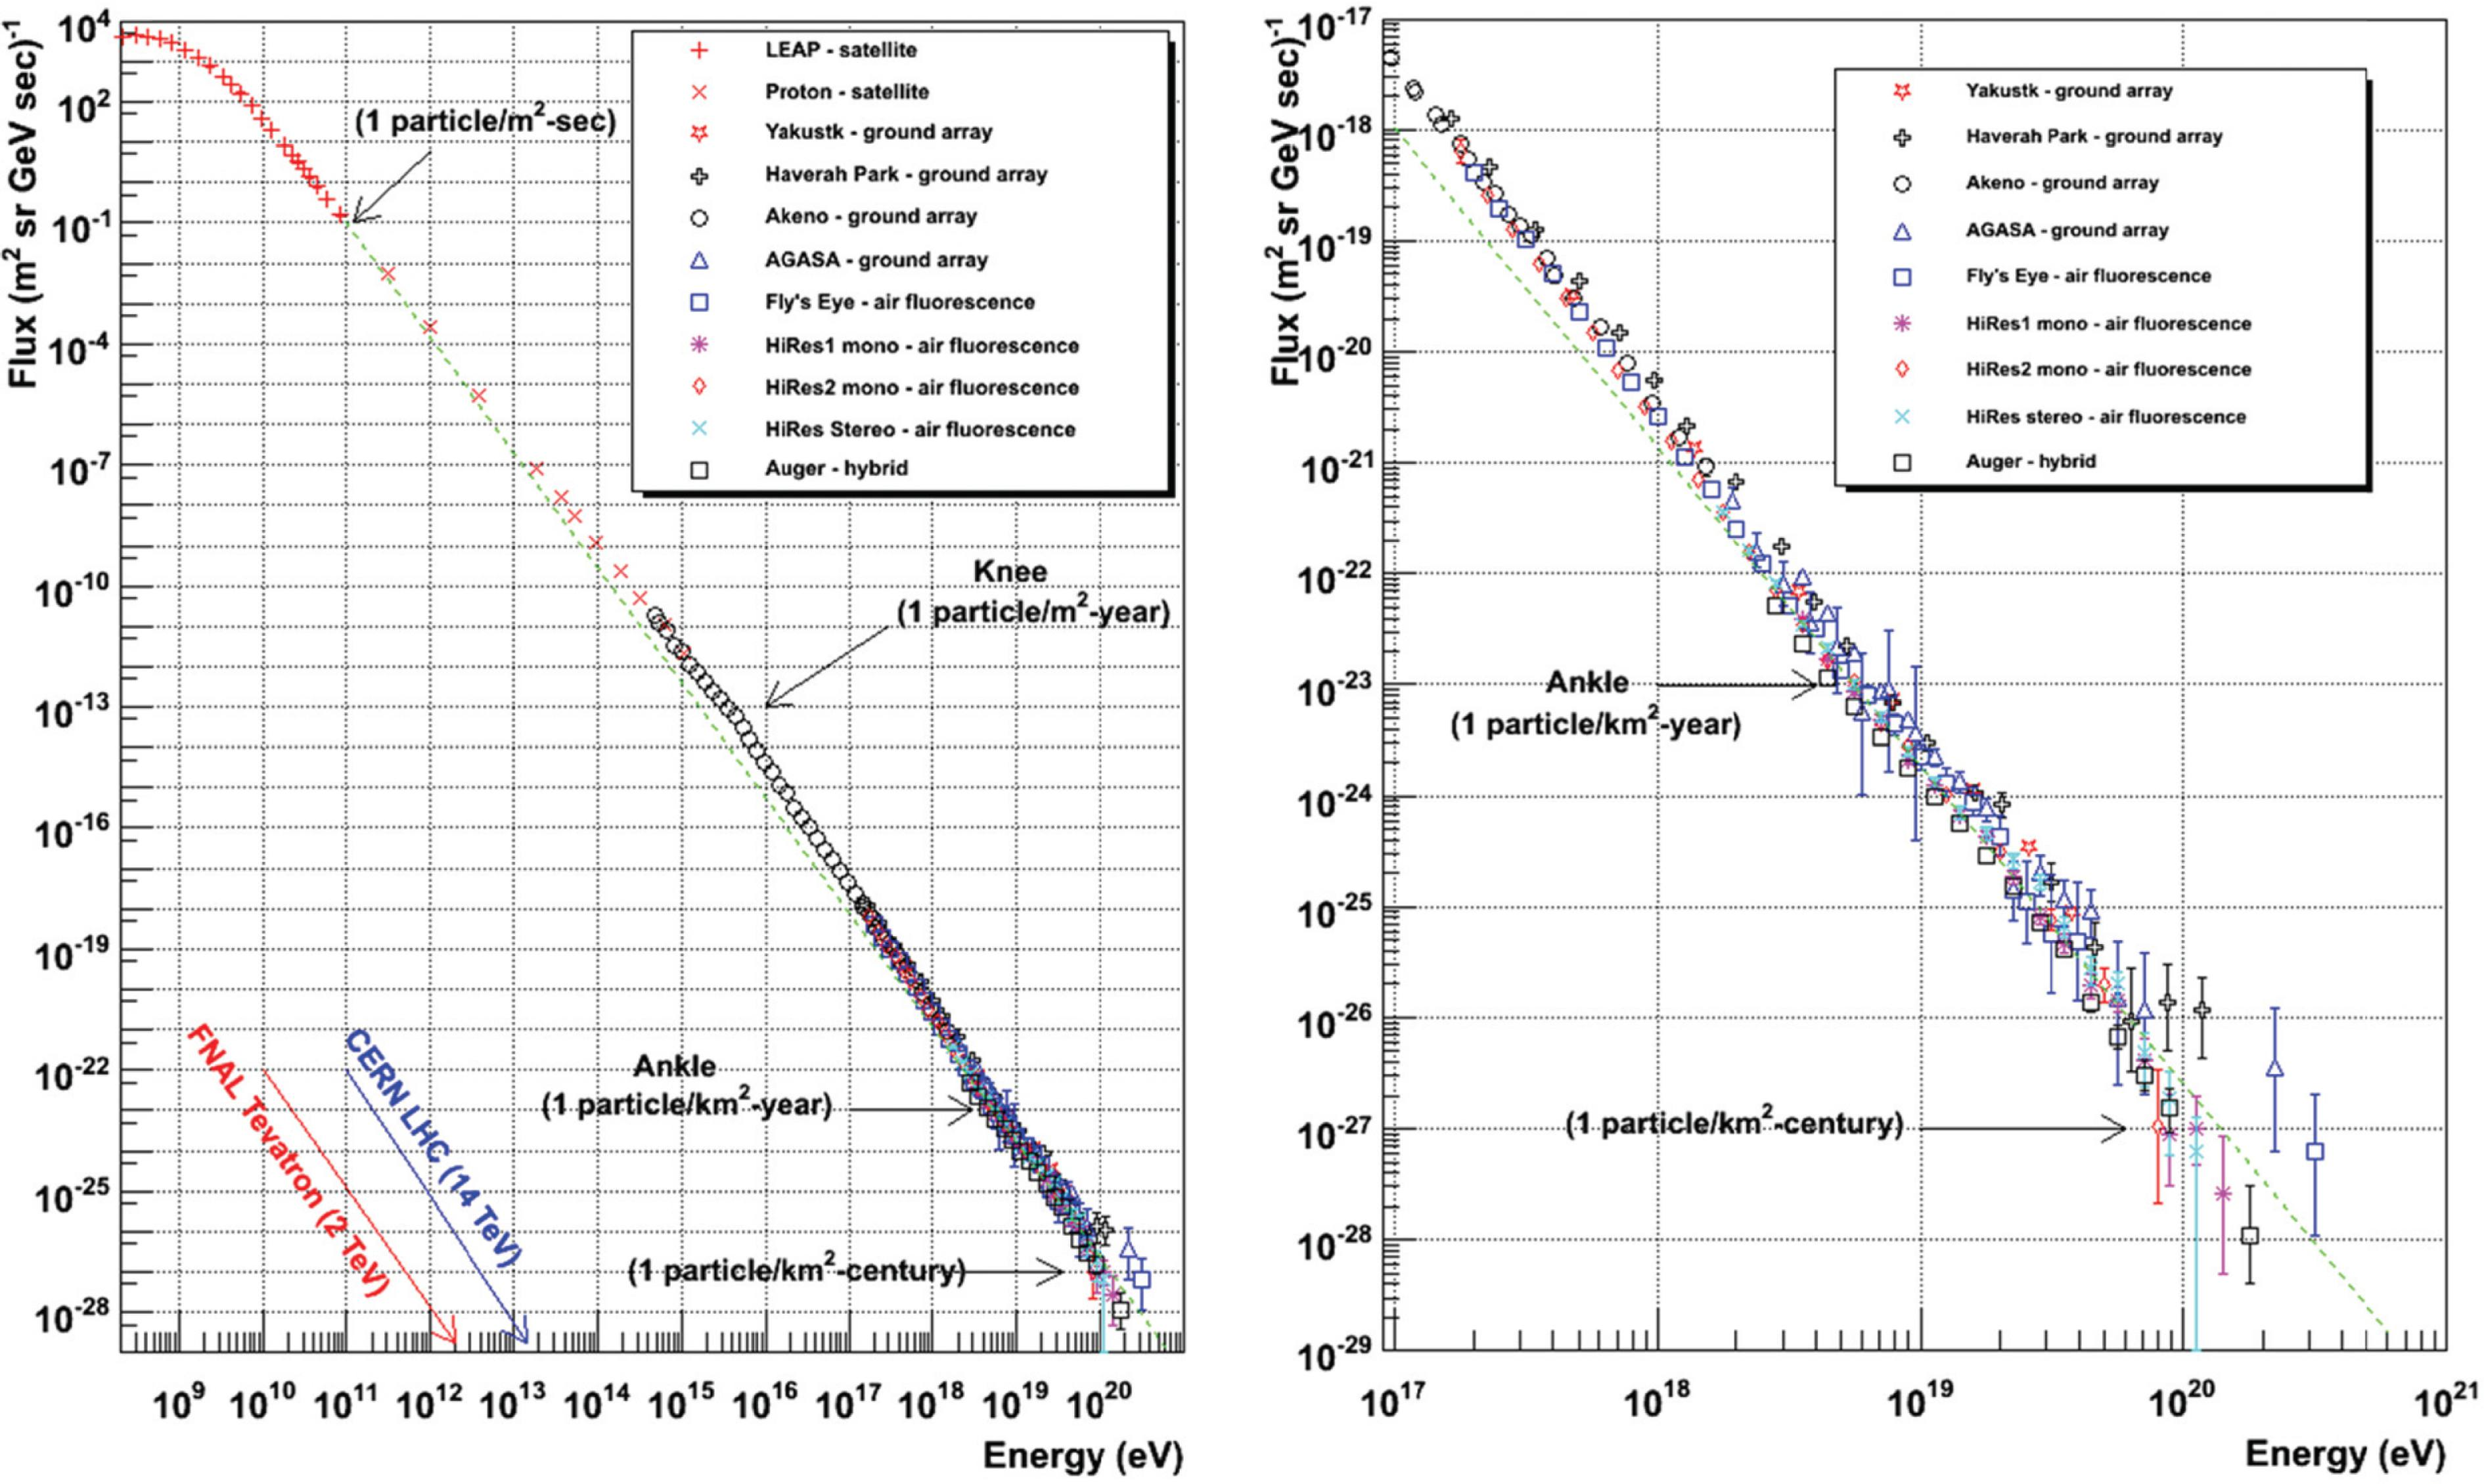
\includegraphics[scale=0.09]{CR_spectrum} 
	
	\caption{Primary cosmic rays flux as a function of the energy [\si{eV}]. To make a comparison, notice that the highest-energy accelerator LHC has a centre of mass energy $\sqrt s = \SI{14}{TeV}$ against $\SI{e20}{eV}$ of maximum energy of cosmic rays. On the other hand at these extreme energies the flux is very low, tipically 1 particle $\si{km^{-2}}$ $\textrm{century}^{-1}$.} \label{CRSpectrum}
\end{figure}

Experimental observations indicate that the differential energy spectrum for primary cosmic rays can be well represented by power-law distributions of the form

\begin{equation}
\frac{\dd N}{\dd E} = k E^{- \gamma}
\end{equation}
where $\gamma$ is the spectral index.
Prominent features in the spectrum are the changes in the slope known as the \emph{knee} at $\SI{e15}{eV}$ and the \emph{ankle} at $\SI{e18}{eV}$ \cite{Longair}.
The spectral index is $\gamma = 2.7$ for energies below the energy of the knee, while for higher energies it changes approximately from $2.7$ to $3$ \cite{Longair}.

\emph{Secondaries} are produced by the interactions of the primaries with the upper Earth's atmosphere\footnote{When discussing the astrophysical origin of cosmic rays, 'secondaries' are those particles produced in interaction of the primaries with the ISM (InterStellar Medium). Nuclei such as lithium, beryllium, and boron are secondaries \cite{PDG}.}.
When primary particles penetrate the atmosphere they interact strongly with air nuclei giving rise to a \emph{hadronic shower} in which pions ($\pi^{\pm}, \pi^0$) are mainly produced, less frequently kaons ($K^{\pm}, K^0$) and even more rarely other hadrons.
Since these particles are unstable they decay into lighter ones, in particular charged kaons and pions decay principally according to the following decay channels 

\begin{equation}
K^+\rightarrow \mu^+ + \nu_{\mu} \qquad
K^-\rightarrow \mu^- + \overline \nu_{\mu} \qquad \tau = \SI{26.03}{ns} \quad \cite{PDG}
\end{equation}

\begin{equation}
\pi^+\rightarrow \mu^+ + \nu_{\mu} \qquad
\pi^-\rightarrow \mu^- + \overline \nu_{\mu} \qquad \tau = \SI{12.38}{ns} \quad \cite{PDG}
\end{equation}
with lifetimes of order $\mathcal{O} (\si{ns})$ and with the production of muons, antimuons and their neutrinos. 
Hadronic collisions produce not only charged pions but also $\pi^0$. The latter decay quickly producing photons ($\pi^0 \rightarrow \gamma \gamma$) which give origin to an \emph{electromagnetic shower}. In fact high-energy photons interact with the nuclei producing an electron-positron pair ($\gamma + N \rightarrow e^+ + e^- + N$) and these leptons in turn can produce photons by bremsstrahlung and so on.

The majority of the decay products cannot reach the Earth's surface since they have a too short lifetime (and not enough energy).
Nevertheless, most of the muons and neutrinos produced by charged pions decay can easily reach the ground due to relativistic effects. 
Therefore muons are the most numerous charged particles
detected at sea level (see Figure \ref{secondary_composition}).
\begin{figure}[!h]
	\centering
	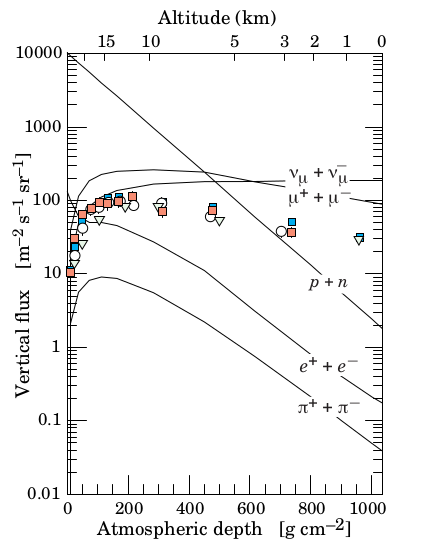
\includegraphics[scale=0.45]{vert_flux} 
	\caption{Vertical fluxes of cosmic rays in the atmosphere with $E > \SI{1}{GeV}$ estimated from nucleon flux. The points show measurements of negative muons with $E_{\mu} > \SI{1}{GeV}$.} \label{secondary_composition}
\end{figure}

Most muons are produced high in the upper atmosphere (typically at $\SI{15}{km}$ altitude) and before reaching the ground they lose about $\SI{2}{GeV}$ due to ionization. Their energy and angular distribution
reflect a convolution of the production spectrum, energy loss in
the atmosphere and decay. 
For example $\SI{2.4}{GeV}$ muons would have a decay length of $\SI{15}{km}$, which is reduced to $\SI{8.7}{km}$ by energy loss.
The mean energy of muons at the ground is $\sim \SI{4}{GeV}$ \cite{PDG}.
%The energy spectrum is almost flat below $\SI{1}{GeV}$, steepens gradually to reflect the primary spectrum in the range 10-100 $\si{GeV}$ and it steepens further at higher energies, since pions with energies greater than the critical energy $\epsilon_{\pi} = \SI{115}{GeV}$ tend to interact in the atmosphere before their decay \cite{PDG}.
%Asymptotically ($E_{\mu} \gg \SI{1}{TeV}$),
%the energy spectrum of atmospheric muons is one power steeper
%than the primary spectrum.\\ 
The flux of vertical muons above $\SI{1}{GeV/c}$ at sea level is $ I_0 \approx 70 \si{m^{-2}} \si{s^{-1}} \si{sr^{-1}}$, which for horizontal detectors is more familiar as

\begin{equation}
\label{mu-rate}
I_0 \approx 1 \si{cm^{-2}} \si{min^{-1}}  \, \cite{PDG} .
\end{equation}

The \emph{muon angular distribution} at the ground as a function of the zenith angle $\theta$ is
\begin{equation} \label{dist}
\frac{\dd N}{\dd \Omega \dd A \dd t} \approx I_0 \cos^2 \theta
\end{equation}
and it is characteristic for muons with $E_{\mu} \sim \SI{3}{GeV}$\footnote{At low energies the angular distribution becomes increasingly steep, while at high energies it flattens, approaching a $\sec \theta$ distribution for $E_{\mu} \gg \epsilon_{\pi} = \SI{115}{GeV}$ and $\theta < \ang{70}$ \cite{PDG}.} \cite{PDG}.
\begin{figure}[!h] 
	\centering
	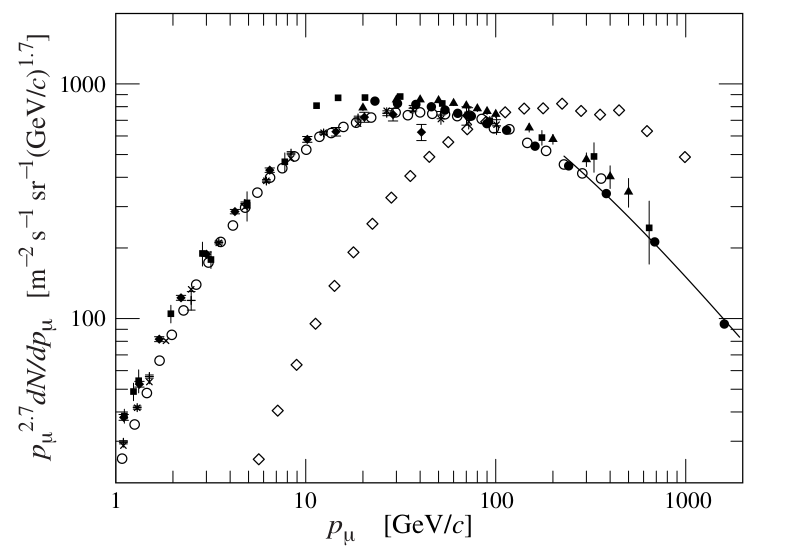
\includegraphics[scale=0.32]{energy_spect} 
	\caption{Spectrum of muons at $\theta = \ang{0}$ ($\blacklozenge , \blacksquare , \blacktriangledown , \blacktriangle , \times , + , \circ, \bullet$) and  $\theta = \ang{75} (\Diamond) $ \cite{PDG}.} \label{energy_spect}
\end{figure}

Figure \ref{energy_spect} shows the muon energy spectrum at sea level for two angles: at large angles the low energy ones decay before reaching the surface, moreover high energy pions decay before they interact, thus the average muon energy increases.

Another important feature of cosmic muons is their measured \emph{charge asymmetry}, which is shown in Figure \ref{muon_asimmetry}. The muon charge ratio $\mu^+ / \mu^-$ reflects either the excess of $\pi^+$ over  $\pi^-$ and
$K^+$ over  $K^-$ in the forward fragmentation region of proton initiated
interactions or the fact that there are more free and bound
protons than free and bound neutrons in the primary spectrum \cite{PDG}. 

\begin{figure}[!h]
	\centering
	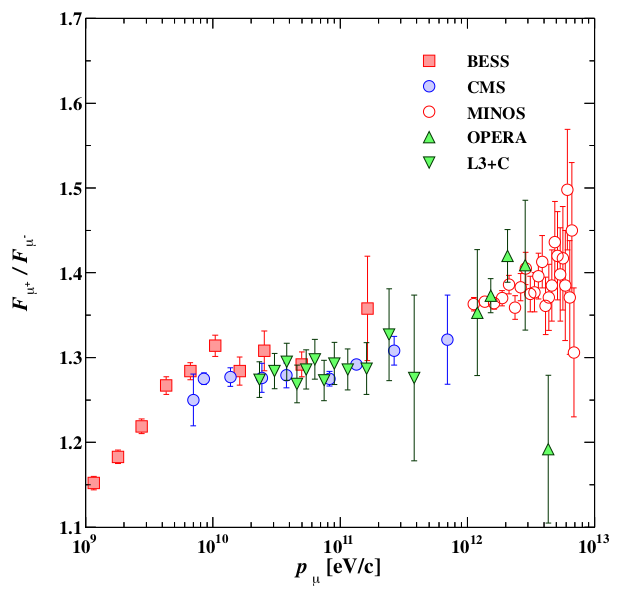
\includegraphics[scale=0.32]{muon_asimmetry} 
	\caption{Muon charge ratio $\mu^+ / \mu^-$ as a function of the muon momentum [\si{eV / c}]. The increase with energy reflects the growing importance of kaons in the $\si{TeV}$ range and it indicates a significant contribution of associated production by cosmic-ray protons ($p \rightarrow \Lambda + K^+ $) \cite{PDG}.} \label{muon_asimmetry}
\end{figure}


\section{Free muon decay}

Muons are unstable particles which decay into electrons with the emission of electron antineutrinos and muon neutrinos\footnote{Positive muons decay in their charged-conjugated final state particles.} according to

\begin{equation} \label{muon decay}
\mu^- \rightarrow e^- + \bar \nu_{e} + \nu_{\mu} \qquad \mu^+ \rightarrow e^+ + \nu_{e} + \bar \nu_{\mu} . 
\end{equation}

The free decay process is described by the Feynman diagram shown in Figure \ref{feynman}.
\begin{figure}[!h]
	\centering	
	
	\begin{tikzpicture}
	\begin{feynman}
	\vertex (a) {\(\mu^{-}\)};
	\vertex [right=of a] (b);
	\vertex [above right=of b] (f1) {\(\nu_{\mu}\)};
	\vertex [below right=of b] (c);
	\vertex [above right=of c] (f2) {\(\overline \nu_{e}\)};
	\vertex [below right=of c] (f3) {\(e^{-}\)};
	
	\diagram* {
		(a) -- [fermion] (b) -- [fermion] (f1),
		(b) -- [boson, edge label'=\(W^{-}\)] (c),
		(c) -- [anti fermion] (f2),
		(c) -- [fermion] (f3),
	};
	
	\end{feynman}
	\end{tikzpicture}
	\caption{Feynman diagram (at LO) for the free muon decay.}\label{feynman}
\end{figure}

The total decay rate $\Gamma$ is given by \cite{Measday}
\begin{equation} \label{Gamma}
\Gamma = \frac{ G_{F}^2 m_{\mu}^5 c^4}{192 \pi^3 \hbar^7} 
\end{equation}
from which we obtain the muon mean lifetime
\begin{equation} \label{tau}
\tau_{\mu} = \frac{1}{\Gamma} = \frac{192 \pi^3 \hbar^7}{ G_{F}^2 m_{\mu}^5  c^4} \simeq \SI{2.2}{\micro\second} .
\end{equation}

The full details of the calculation of the decay rate are reported in Appendix \ref{Appendix A}.
A most accurate value for the total decay rate can be calculated taking into account QED radiative corrections and the effects of the finite mass of the electron \cite{Measday}
\begin{equation}
\Gamma_{\mu} =  \frac{ G_{F}^2 m_{\mu}^5 c^4}{192 \pi^3 \hbar^7} \left[ 1 - \frac{\alpha}{2 \pi} \left( \pi^2 - \frac{25}{4} \right) \right] \emph{f} \left( \frac{m_{e}^2}{m_{\mu}^2} \right) 
\end{equation}
where
\begin{equation}
\emph{f} \left( \frac{m_{e}^2}{m_{\mu}^2} \right) = \emph{f} (x) = 1 - 8x - 8 x^3 - x^4 + 12 x^2 \ln(\frac{1}{x}) .
\end{equation}

Therefore, taking into account these corrections\footnote{The radiative correction gives a coefficient of $0.995796$ while the finite mass correction is $0.999813$, giving a total correction of $0.995610$.}, the total decay rate is given by \cite{Measday}
\begin{equation}
\Gamma_{\mu} = \frac{1}{\tau_{\mu}}=  0.995610 \frac{ G_{F}^2 m_{\mu}^5 c^4}{192 \pi^3 \hbar^7} .   
\end{equation}

$\Gamma_{\mu}$ has been computed considering only the leading muon decay mode $\mu^- \rightarrow e^- \bar \nu_{e} \nu_{\mu}$, since its branching ratio is $\approx 100 \%$. Actually muons can decay even according to $\mu^- \rightarrow e^-  \bar \nu_{e}  \nu_{\mu} \gamma$
and $\mu^- \rightarrow e^-  \bar \nu_{e}  \nu_{\mu} e^+ e^-$ with branching ratios of $(6.0 \pm 0.5) \cdot 10^{-8}$ and $(3.4 \pm 0.4) \cdot 10^{-5}$ respectively \cite{PDG}; therefore we can neglect the contributions of these decay channels. 
The most accurate experimental value for the muon mean lifetime is 
\begin{equation}
\tau_{\mu} = (2.1969811 \pm 0.0000022) \cdot 10^{-6} \, \si{s} .  \, \cite{PDG}
\end{equation}

Therefore the theoretical prediction for the muon lifetime of Eq. \eqref{tau} is consistent with the experimental results.

\section{Muon decay in matter}

When $\mu^{\pm}$s travel through a material medium they behave differently depending on their charge:
this different behaviour when they are stopped in matter is responsible for a difference in positive/negative $\mu$ lifetime measurements.\\ 
Since positive muons have a repulsive interaction with atomic nuclei they can cross the medium and lose energy by ionization and decay almost at rest. For this reason their lifetime is similar to the one of free muons.  On the other hand, negative muons feel the electrostatic attraction from the nuclei and can be bind by the material atoms making a $\emph{muonic atom}$. In this
case the muon can decay as if it were approximately free or it can be captured by the nuclei.\\ 
%If the muon binds in a non-K shell it emits X rays until it reaches the K shell. 
The \emph{nuclear muon capture} is a process in which a proton captures a negative muon producing a neutron and a neutrino according to the reaction

\begin{equation}
	\mu^- + p   \rightarrow n + \nu_{\mu}
\end{equation}
that is represented by the Feynman diagram in Fig. \ref{buond muon decay}.


\begin{figure}[!h]
	\centering	
	
	\begin{tikzpicture}
	\begin{feynman}
	\vertex (d1) {\(d\)}; 
	\vertex[right=5cm of d1] (d2) {\(d\)};
	\vertex[below right=1cm and 2.5cm of d1] (vert1); 
	\vertex[below=4mm of d1] (u1) {\(u\)}; 
	\vertex[right=5cm of u1] (u2) {\(u\)};
	\vertex[below right=1cm and 2.5cm of u1] (vert2); 
	\vertex[below=4mm of u1] (u3) {\(u\)}; 
	\vertex[right=5cm of u3] (d3) {\(d\)};
	\vertex[below right=1cm and 2.5cm of u3] (v1);
	\vertex[below=1.5cm of v1] (v2);
	\vertex[below=4.5cm of d2] (nu) {$\nu_{\mu}$};
	\vertex[below=4.5cm of d1] (mu) {${\mu}^-$};
	\diagram* { {[edges=fermion]
			(d1) -- (vert1) -- (d2), 
			(u1) -- (vert2) -- (u2),
			(u3) -- (v1) -- (d3), (mu) -- (v2) -- (nu)},
		(v1) -- [boson, edge label=\(W^-\)] (v2)
	};
	\draw [decoration={brace}, decorate,] (u3.south west) -- (d1.north west) node [pos=0.5, left=0.18cm] {\(p\)};
	\draw [decoration={brace}, decorate] (d2.north east) --  (d3.south east) node [pos=0.5, right=0.18cm] {\(n\)};
	\end{feynman} 
	\end{tikzpicture}
	
	\caption{Feynman diagram (at LO) for the nuclear muon capture.}\label{buond muon decay}
\end{figure}
\noindent If the muon were captured by a proton at rest, the energy of the neutrons produced in the reaction would be approximately $\SI{5.2}{MeV}$. Since, however, the nucleons are in constant motion, the neutron energy may reach a few tens of $\si{MeV}$. Either fast neutrons leave the nucleus, or they eject a particle by means of a direct interaction, or they transfer their energy to other nucleons exciting them \cite{Weissenberg}.
The emission of protons and other charged particles subsequently to the nucleon excitation is impeded by the Coulomb barrier, therefore particles emitted during this process are mainly neutrons and $\gamma$ rays\footnote{Another possible interaction which may happen is the \emph{radiative $\mu^-$ capture by the nuclei}. In this case electromagnetic radiation is emitted after the muon capture by nuclei according to the reaction
	$p + \mu^- \rightarrow n + \nu_{\mu} + \gamma$. The photon spectrum produced as a result of nuclear $\mu^-$ capture exhibits a maximum at $\SI{30}{MeV}$ and extends up to $\SI{100}{MeV}$.  
	This process is rare since the total probability of radiative $\mu^-$ capture is about $10^{-4}$ with respect to the total probability of $\mu^-$ capture, i.e.  $\Gamma_{rad} \approx 10^{-4} \, \Gamma_{c}$, 
	where $\Gamma_{rad}$ is the radiative capture rate and $\Gamma_{c}$ is the non-radiative one \cite{Weissenberg}.}\cite{Weissenberg}.\\

\noindent A negative muon in the K shell of a muonic atom can either decay or be captured by the nuclei, hence the total decay rate for a $\mu^-$ in matter is given by the sum of the $\Gamma$ given by nuclear capture and the bound decay 
\begin{equation} \label{piripirlo}
	\Gamma_{tot} = \Gamma_{capt} + \Gamma_{bound} = \Gamma_{capt} +  Q \cdot \Gamma_{decay} \, \cite{Measday}
\end{equation}
where $\Gamma_{tot} = (\tau_{\mu^-})^{-1}$ and $\Gamma_{decay} = (\tau_{\mu^+})^{-1}$ and Q is the Huff factor, which is a small correction
which takes into account the fact that the normal muon decay rate is reduced for a bound $\mu^-$ \cite{Measday}. In fact there is a difference between the decay probability for a free muon and a muon in the K shell of a muonic atom which is due to different effects. Firstly, the total energy of the bound negative muon is less than the total energy of the free positive one because of the binding energy.
Consequently the phase space accessible to the decay particles is reduced, hence the total decay probability is reduced. Secondly, the motion of negative muons in the K shell gives rise to a relativistic change in the time scale, increasing the life-time in the laboratory frame (decreasing the decay probability). Finally, the effect of the nuclear Coulomb field may influence the decay probability \cite{Weissenberg}.
An estimation of the $\Gamma_{decay}(Z)$ decreasing is:

\begin{equation}
	\Gamma_{decay}(Z) \approx \left[ 1 - \beta \left( \frac{Z}{137} \right)^2 \right] \cdot \Gamma_{decay} (0) \, \cite{Weissenberg}
\end{equation}
where $\beta \approx 3$ if  time dilation effect is taken into account. 
In general, the higher the nucleus atomic number Z is, the more probable muon capture is, since the increasing of Z reduces the atomic orbital radius and
enhances the probability that the muon could be found in the nucleus.
The muon capture probability is given by the \emph{Primakoff formula} 

\begin{equation}
	\Gamma_{capt}(Z) = Z_{eff}^4 X_1 \left( 1 - X_2 \frac{A - Z}{2A} \right)  \, \cite{Measday}
\end{equation}
where $X_1$ is the muon capture rate for hydrogen %\footnote{Actually it is reduced because the neutrino has less energy for nuclear capture.}
while the $X_2$ term takes into account the Pauli exclusion
principle.
For the Primakoff formula a typical fit gives $X_1 = \SI{170}{s^{-1}}$ and $X_2 =3.125$ \cite{Measday}.
The effective nucleus electric charge $Z_{eff}$ takes into account the finite dimension of nucleui, since heavy nuclei cannot be described as point charges, and it can be estimated thanks to the following expression \cite{Weissenberg}:
\begin{equation}
	Z_{eff} = Z \left[ 1 + \left( \frac{Z}{42} \right)^{1.47} \right]^{-\frac{1}{1.47}} \, \cite{Weissenberg}   
\end{equation}
Experimental decay and capture rates for different materials are reported in Tab. \ref{tabellina}.
Referring to elements with low atomic number, e.g. carbon, the nuclear $\mu^-$-capture probability is much smaller than the decay probability, and the negative-muon lifetime $\tau_{\mu^-}$ is nearly equal to the lifetime of a free positive muon.\\
Finally, since negative muons in matter can decay in a bound state or be captured by nuclei, their measured lifetime in matter is different from the one of antimuons, which decay in matter with lifetime equal to the one of the free decay.

\begin{table} 
	\centering
	\begin{tabular}{ccccc} 
		\toprule
		Element & Z & $\Gamma_{d} \, [10^5 \, \si{s^{-1}} ]$ & $\Gamma_{tot} \, [10^5 \, \si{s^{-1}} ]$ & $\tau \, [\si{ns}]$ \\
		\midrule
		C   & 6    & $0.36 \pm 0.01$ & $3.97 \pm 0.01$ \cite{sutton} & $2025 \pm 4$ \cite{sutton}\\
		Na   & 11    & $3.87 \pm 0.15$ & $8.40 \pm 0.14$ & $1190 \pm 20$\\
		Al   & 13 & $6.91 \pm 0.20$ & $11.40 \pm 0.13$ & $880 \pm 10$\\
		Cl   & 17 & $13.9 \pm 0.9$ & $18.5 \pm 0.68$ & $540 \pm 20$\\
		Pb   & 82 & $129 \pm 5$ & $133.0 \pm 5.8$ & $75 \pm 3 $\\
		\bottomrule
	\end{tabular} 
	\caption{Experimental decay and capture rates in different materials for negative muons \cite{Weissenberg}.}\label{tabellina}
\end{table}


\section{Interaction muon-scintillator}
\label{Mu-Sci}

When muons reach the ground and cross an absorber they lose some of their energy through scattering with electrons. The energy loss per mass thickness is about the same in any material and for a massive charged particle ($m_{\mu} \gg m_{e}$) is well described by the Bethe-Bloch formula \cite{PDG}
\begin{equation}
\left< - \frac{\dd E}{\dd \rho x} \right> = 4 \pi N_{A} r_{e}^2 m_e c^2  \frac{Z}{A} \frac{z^2}{\beta^2} \left[ \frac{1}{2} \ln \frac{2 m_e c^2 \beta^2 \gamma^2 W_{max}}{I^2} - \beta^2 - \frac{\delta(\beta \gamma)}{2} \right] .
\end{equation}

Since muons reach the ground with a mean energy of $\SI{4}{GeV}$ they are \emph{minimum ionizing particles} and their average energy loss in matter is about $ \SI{2}{MeV} \, \si{g}^{-1} \, \si{cm}^{2}$.    
Therefore, when muons cross plastic scintillators having the same thicknesses they lose the same mean fraction of total energy.
Plastic scintillators with thicknesses of $\SI{1}{cm}$ and $\SI{4}{cm}$ are included in our experimental equipment (see Section \ref{expeq}) and the corresponding mean energy released is about $2$ and $\SI{8}{MeV}$ respectively\footnote{Plastic scintillators densities range from $1.03$ to $\SI{1.20}{g / cm^{3}}$ \cite{PDG}.}.\\

Plastic scintillators do not respond linearly to ionization density. Very dense ionization columns emit less light than expected on the basis of $\dd E / \dd x$ for minimum ionizing particles \cite{PDG}. The response of organic scintillators to charged particles can be described assuming that a high ionization density along the track of the particle leads to quenching from damaged molecules and to a lowering of the scintillation efficiency \cite{Knoll}.
Quenching effects %between the excited molecules 
reduce the light yield according to \emph{Birks' formula} 
\begin{equation}
\frac{\dd L}{\dd x} = \frac{ S\cdot \displaystyle\frac{\dd E}{\dd x} }{ 1 + k B \cdot\displaystyle \frac{\dd E}{\dd x} } 
\end{equation}
where $L$ is the luminescence, $S$ is the normal scintillation efficiency at low specific ionization density,
and $kB$ is Birks’ constant\footnote{Assuming that the density of damaged molecules along the wake of the particle is directly proportional to the ionization density, we can represent their density by $B \, \dd E / \dd x$, where B is a proportionality constant. Birks assumed that some fraction $k$ of these will lead to quenching \cite{Knoll}.}, which must be determined for each detector by measurements.\\

The energy deposit in the scintillating organic compound excites molecular levels which rapidly de-excites emitting UV photons. Typical photon yields are about 1 photon per
100 eV of energy deposit \cite{PDG}. Therefore the scintillators used in this experiment, when crossed by MIPs, will yield about $2 \cdot 10^4$ or $8 \cdot 10^4$ photons respectively. Using wavelength shifters UV photons are converted into visible light, which is optically collected and absorbed by the photocatode in order to extract photoelectrons.
The resulting photoelectrons signal will
depend on the collection and transport efficiency of the optical package but even on the quantum
efficiency of the photodetector \cite{PDG} (typically $20-30\%$ \cite{Knoll}). Considering a PhotoMultiplier Tube (PMT) made by 10 dynodes with a gain $\delta \sim 4$ each, its total gain is about $ G = \delta^{10} \sim 4^{10} \sim 10^6$. Therefore at the anode a great number of secondary electrons are collected giving a significant signal.

Since in our experimental equipment scintillators of different thicknesses are used, the different amount of the energy loss during the interaction muons-detectors clearly entails different pulse heights for the PMT output signal observable on an oscilloscope.

Concerning the timing response, plastic scintillators have decay times of order $\mathcal{O}(\si{ns})$ while rise times are much faster.
Therefore the fast timing response of plastic scintillators allows fast timing resolution measurements.

\section{Experimental equipment} \label{expeq}
\subsection{Scintillators} \label{scintillators}

The aim of the experiment is to achieve a measurement of the muons mean lifetime thus, a detector with fast response (order of ns) is required. For this reason organic scintillators are used and their fluorescence emission reaches photomultipliers in order to convert the light into an electrical signal.
In this experiment three scintillators have been used: \emph{Minosse}, \emph{Caronte} and \emph{Cerbero} (see Figure \ref{rivelatori}).
\begin{itemize}
	\item \emph{Minosse}:  $800\times 300\times\SI{38}{mm}^3$ EJ200 SCIONIX
	\item \emph{Caronte}:  $800\times 300\times\SI{38}{mm}^3$ BC408 Saint Gobain
	\item \emph{Cerbero}:  $800\times 300\times\SI{10}{mm}^3$ BC408 Saint Gobain
\end{itemize}
\emph{Cerbero} is the only detector which has a light guide.

\begin{figure}[!h]
	\centering
	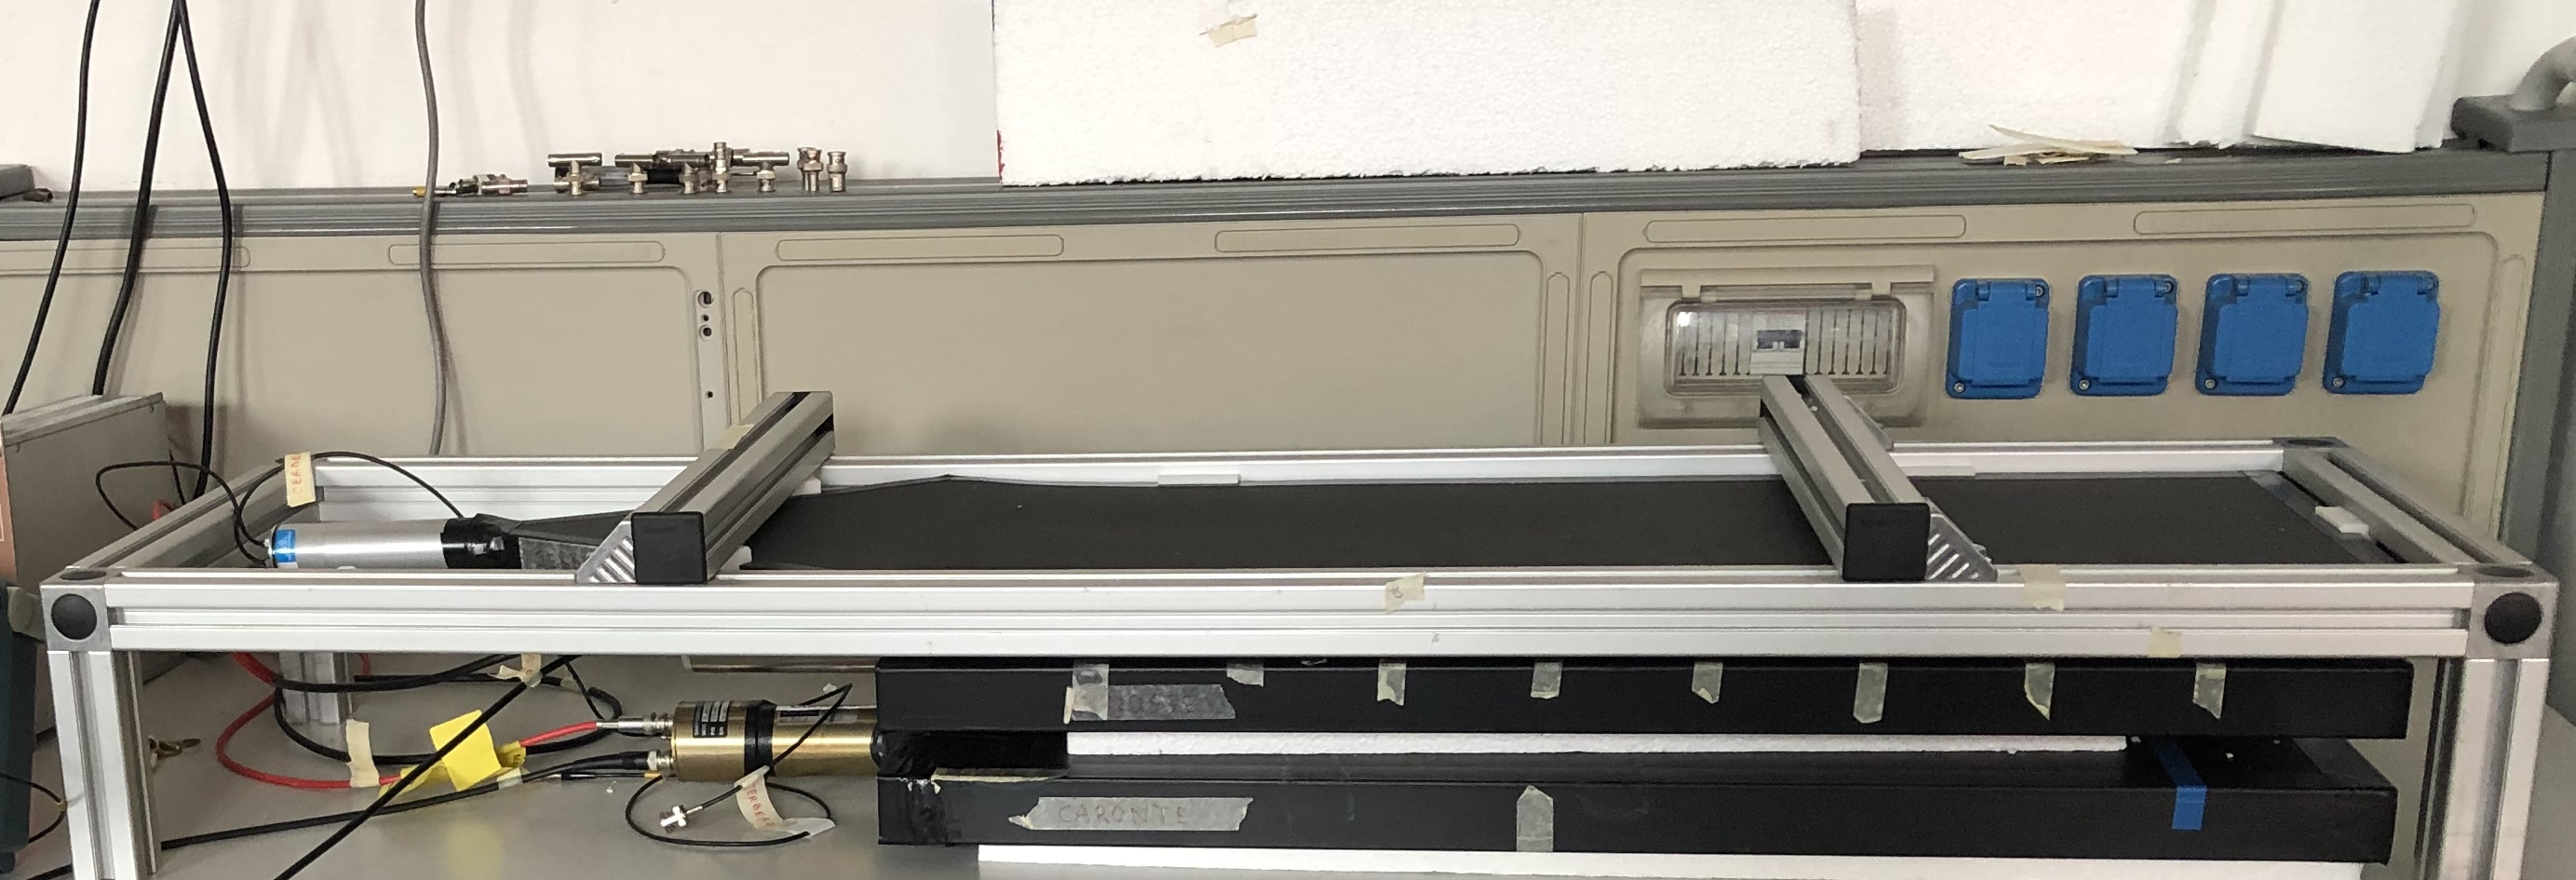
\includegraphics[width=\linewidth]{riv}
	\caption{Plastic scintillators.}
	\label{rivelatori}
\end{figure}

\subsection{Electronic instrumentation } \label{Electronic instrumentation}

The electronic instrumentation used during the whole experiment is:
\begin{itemize}
	\item NIM Crate (CAEN)
	\item Quad Scaler And Preset Counter/Timer N1145 (CAEN)
	\item Programmable Logic Unit N81 (CAEN)
	\item NIM Model 622 Quad 2-Fold Logic Unit(LeCroy)
	\item Dual Delay Unit N108 (CAEN)
	\item Dual Timer N93 (CAEN)
	\item Logic FAN-IN FAN-OUT N454 (CAEN)
	\item Discriminator N417 (CAEN)
	\item 2CH High Voltage Power Supply N1495 (CAEN)
	\item High Voltage Power Supply N556 (ORTEC)
	\item Desktop Digitizer (CAEN)
\end{itemize}

\chapter{Monte Carlo simulations}  
\section{Geometric factor} \label{sec:geometric factor}

The flux of vertical muons whose momentum is greater than $\SI{1}{GeV/c}$ at sea level is $ I_0 \approx 70 \ \si{m^{-2}} \si{s^{-1}} \si{sr^{-1}}$ (see Section \ref{sec:introduction}) but this value refers to a single detector. However, the next working conditions require that the three scintillators to be employed in a coincidence state, forming a particle telescope \cite{Sullivan}, hence it is natural to expect a decrease in the radiation intensity detected, with respect to the nominal one. It is possible to estimate the intensity of radiation $I_0$ given the coincidence counting rate and the parameters (e.g. detectors dimensions) of our configuration. Since the calculus that follows has been done for an ideal telescope (i.e. the detection efficiency is $1$ for particles in a given energy range and $0$ otherwise), some assumption have been made: 
\begin{enumerate}
	\item Incident particles have rectilinear trajectories.
	\item The surface of the detectors considered has no thickness.
\end{enumerate}
The former can be reasonably accepted because in this experiment the particles that interact with the detectors are muons with a mean energy of $\sim \SI{4}{GeV}$ (see Section \ref{sec:introduction}). Nevertheless, the latter plays an important role since thickness is not negligible. So a Monte Carlo simulation has been performed to analyze if these assumptions are somewhat acceptable.\\
\indent If we consider an isotropic radiation $I=I_0$, the proportionality coefficient between the intensity $I$ and the coincidence rate $C$ is the \emph{geometric factor} $G$ of the telescope: $I\equiv I_0 = C/G$. Nevertheless, in this specific case the intensity of the particles distribution is not isotropic: $I = I_0\cdot \cos^2\theta$ \cite{PDG}. Therefore, a correction is needed when evaluating the geometric factor. However, in both cases the geometric factor has the unit of $\left[ \si{\meter}^{2}\cdot \si{\steradian}\right] $ and it is clear that this quantity represents the geometric acceptance of the particle telescope.\\
This value can be derived analytically for certain configurations \cite{Thomas} both for an isotropic and a $\cos^2\theta$-distributed intensity. In our case we have three rectangular scintillators one over the other but only the position and the dimensions of the first and the third detector affect the estimation of the geometrical factor. This assumption is justified due to the fact that the middle scintillator does not change the field of view of the telescope.
\begin{figure}[!htp]
	\centering
	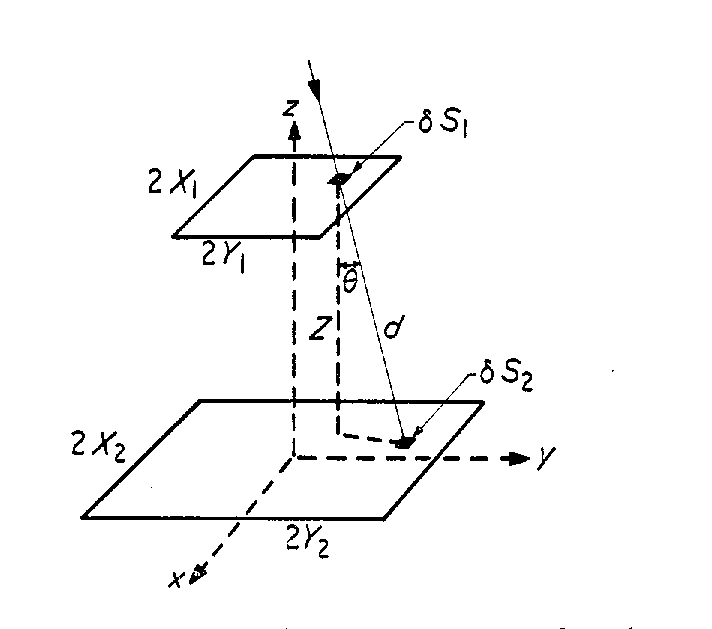
\includegraphics[height=5cm]{Thomas}
	\caption{Scheme of a particle telescope with two rectangular detectors.}
	\label{fig:Thomas}
\end{figure}
Referring to Figure \ref{fig:Thomas}, if we consider a telescope made of two rectangular detectors with sides $(2X_1,2Y_1)$ and $(2X_2,2Y_2)$ and a separation between them equal to $Z$, it is possible to obtain the explicit formula of the geometric factor\footnote{Considering a $\cos^2\theta$ distribution.}:
\begin{align}\label{eq:Thomas}
	G & = \frac{Z^2 + 2\left( X_1+X_2\right) ^2}{2\left[ Z^2 + \left( X_1+X_2\right)^2 \right] ^{\frac{1}{2}}} \cdot \left[ \left(Y_1+Y_2\right)\arctan\frac{Y_1+Y_2}{\left[ Z^2 + \left( X_1+X_2\right)^2 \right]^{\frac{1}{2}}} \right. \nonumber \\
	& \qquad \qquad \qquad \qquad \left. - \left(Y_2-Y_1\right)\arctan\frac{Y_2-Y_1}{\left[ Z^2 + \left( X_1+X_2\right)^2 \right]^{\frac{1}{2}}}\right] \nonumber \\
	%
	%Second term
	%
	&  - \frac{Z^2 + 2\left( X_2-X_1\right) ^2}{2\left[ Z^2 + \left( X_2-X_1\right)^2 \right] ^{\frac{1}{2}}} \cdot \left[ 	\left(Y_1+Y_2\right)\arctan\frac{Y_1+Y_2}{\left[ Z^2 + \left( X_2-X_1\right)^2 \right]^{\frac{1}{2}}} \right. \nonumber \\
	& \qquad \qquad \qquad \qquad \left. - \left(Y_2-Y_1\right)\arctan\frac{Y_2-Y_1}{\left[ Z^2 + \left( X_2-X_1\right)^2 \right]^{\frac{1}{2}}}\right] \nonumber \\
	%
	%Third term
	%
	& + \frac{Z^2 + 2\left( Y_1+Y_2\right) ^2}{2\left[ Z^2 + \left( Y_1+Y_2\right)^2 \right] ^{\frac{1}{2}}} \cdot \left[ \left(X_1+X_2\right)\arctan\frac{X_1+X_2}{\left[ Z^2 + \left( Y_1+Y_2\right)^2 \right]^{\frac{1}{2}}} \right. \nonumber \\
	& \qquad \qquad \qquad \qquad \left. - \left(X_2-X_1\right)\arctan\frac{X_2-X_1}{\left[ Z^2 + \left( Y_1+Y_2\right)^2 \right]^{\frac{1}{2}}}\right] \nonumber \\
	%
	%Fourth term
	%
	&  - \frac{Z^2 + 2\left( Y_2-Y_1\right) ^2}{2\left[ Z^2 + \left( Y_2-Y_1\right)^2 \right] ^{\frac{1}{2}}} \cdot \left[ \left(X_1+X_2\right)\arctan\frac{X_1+X_2}{\left[ Z^2 + \left( Y_2-Y_1\right)^2 \right]^{\frac{1}{2}}} \right. \nonumber \\
	& \qquad \qquad \qquad \qquad \left. - \left(X_2-X_1\right)\arctan\frac{X_2-X_1}{\left[ Z^2 + \left( Y_2-Y_1\right)^2 \right]^{\frac{1}{2}}}\right]
\end{align}
Since all of the three scintillators have the same width and length: $X_1 = X_2 = X$ and $Y_1 = Y_2 = Y$. Hence, it is clear that
\begin{equation}
	\begin{cases}\label{eq:condG_simplified}
		X_1 + X_2 = 2X \\
		Y_1 + Y_2 = 2Y \\
		X_2 - X_1 = 0 \\
		Y_2 - Y_1 = 0
	\end{cases}
\end{equation}
and thus it is possible to simplify \eqref{eq:Thomas} obtaining
\begin{align}\label{eq:Thomas_simplified}
	G & = \frac{Z^2 + 8X^2}{2\left( Z^2 + 4X^2 \right) ^{\frac{1}{2}}} \cdot \left[ 2Y\arctan\frac{2Y}{\left( Z^2 + 4X^2 \right)^{\frac{1}{2}}} \right]
	%
	%Second term
	%
	- \frac{Z}{2} \cdot \left( 2Y\arctan\frac{2Y}{Z} \right) \nonumber \\
	%
	%Third term
	%
	& + \frac{Z^2 + 8Y^2}{2\left( Z^2 + 4Y^2 \right) ^{\frac{1}{2}}} \cdot \left[ 2X\arctan\frac{2X}{\left( Z^2 + 4Y^2 \right)^{\frac{1}{2}}} \right]
	%
	%Fourth term
	%
	- \frac{Z}{2} \cdot \left( 2X\arctan\frac{2X}{Z} \right)
\end{align}
Using the coincidence counting rate `$C$'\footnote{It has been estimated as the double coincidences mean value.} given by the upper and the lower scintillators and the geometric factor calculated thanks to \eqref{eq:Thomas_simplified}, we can evaluate the intensity of the particles flux detected. In particular the intensity has been estimated as in \eqref{eq:intensity} where not only the coincidence rate and the geometric factor are present but also the efficiency of our telescope has been taken into account.
\begin{equation}\label{eq:intensity}
	I = \frac{C}{G\cdot\varepsilon_1 \varepsilon_2} \equiv \frac{C}{G\cdot\varepsilon_t}
\end{equation}
where $\varepsilon_1, \varepsilon_2$ are the efficiencies of the upper and lower detector and $\varepsilon_{t} = \varepsilon_1 \varepsilon_2$ is the overall efficiency of the particle telescope.
\begin{figure}[!htp]
	\centering
	\begin{subfigure}{.3\textwidth}
		\centering
		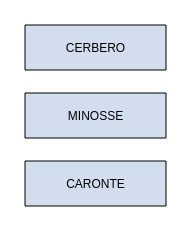
\includegraphics[width=.7\textwidth]{layout1}
		\caption{Layout 1}\label{subfig:l1}
	\end{subfigure}\hfill
	\begin{subfigure}{.3\textwidth}
		\centering
		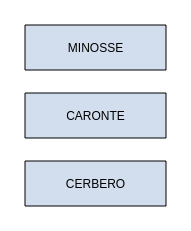
\includegraphics[width=.7\textwidth]{layout3}
		\caption{Layout 2}\label{subfig:l2}
	\end{subfigure}\hfill
	\begin{subfigure}{.3\textwidth}
		\centering
		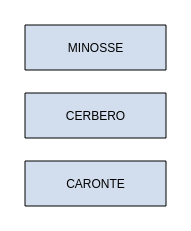
\includegraphics[width=.7\textwidth]{layout2}
		\caption{Layout 3}\label{subfig:l3}
	\end{subfigure}
	\caption{All the possible configurations with three detectors. Note that the exchange of the external scintillators does not affect the geometric factor.}
	\label{fig:telescopes_layout}
\end{figure}
Results (with respect to Figure \ref{fig:telescopes_layout}) are reported in Table \ref{tab:intensities},
\begin{table}[!htp]
	\centering
	\begin{tabular}{r|ccc}
		\toprule
		& $C \ \left[ \si{\second}^{-1}\right] $ & $G \ \left[ \si{\meter}^{2}\cdot \si{\steradian}\right] $ & $I \ \left[ \si{\meter}^{-2} \cdot \si{\second}^{-1} \cdot \si{\steradian}^{-1}\right] $\\
		\midrule
		Layout 1 & $22.5$ & $0.3112$ & $73.17$\\
		Layout 2 & $18.6$ & $0.3112$ & $60.32$\\ 
		Layout 3 & $18.7$ & $0.2602$ & $72.90$\\
		\bottomrule
	\end{tabular}
	\caption{Incident particles intensities for the three possible configurations.}
	\label{tab:intensities}
\end{table}
where we can see that the $G$ factor, as well as the distance\footnote{The dead layer of the detectors has been taken into account during the estimation of the distance.} $Z$ between the upper scintillator and the lower one (see Table \ref{tab:set-up}), is the same for Layout 1 and 2, but different from the third one.
\begin{table}[!htp]
	\centering
	\begin{tabular}{cc}
		\toprule
		Variable & Value ($\si{\meter}$)\\
		\midrule
		$2X_1$ & $0.800 \pm 0.001$\\
		$2Y_1$ & $0.300 \pm 0.001$\\
		$2X_2$ & $0.800 \pm 0.001$\\
		$2Y_2$ & $0.300 \pm 0.001$\\
		$Z$ & $0.080 \pm 0.005$\\
		\bottomrule
		&\\
		\multicolumn{2}{c}{\footnotesize (a) \emph{Layout 1}}
	\end{tabular}\hfill
	\begin{tabular}{cc}
		\toprule
		Variable & Value ($\si{\meter}$)\\
		\midrule
		$2X_1$ & $0.800 \pm 0.001$\\
		$2Y_1$ & $0.300 \pm 0.001$\\
		$2X_2$ & $0.800 \pm 0.001$\\
		$2Y_2$ & $0.300 \pm 0.001$\\
		$Z$ & $0.080 \pm 0.005$\\
		\bottomrule
		&\\
		\multicolumn{2}{c}{\footnotesize (a) \emph{Layout 2}}
	\end{tabular}\hfill
	\begin{tabular}{cc}
		\toprule
		Variable & Value ($\si{\meter}$)\\
		\midrule
		$2X_1$ & $0.800 \pm 0.001$\\
		$2Y_1$ & $0.300 \pm 0.001$\\
		$2X_2$ & $0.800 \pm 0.001$\\
		$2Y_2$ & $0.300 \pm 0.001$\\
		$Z$ & $0.150 \pm 0.005$\\
		\bottomrule
		&\\
		\multicolumn{2}{c}{\footnotesize (a) \emph{Layout 3}}
	\end{tabular}
	\caption{Geometrical parameters of the detectors setup. $Z$ represents the distance between the upper and the lower detectors while the couple $\left(2X_{1/2}, 2Y_{1/2}\right)$ are the length and width, respectively, of the scintillators.}
	\label{tab:set-up}
\end{table}
Now it is possible to propagate the errors both in \eqref{eq:Thomas_simplified} and in the evaluation of the intensities \eqref{eq:intensity}.\\
The errors propagation formula for a general function $f = f\left( x_1, x_2, \dots, x_n\right)$ is
\begin{equation}\label{eq:error_propagation}
	\sigma_f = \sqrt{\sum_{i = 1}^{n}\left( \frac{\partial f}{\partial x_i}\cdot \sigma_{x_i}\right)^2 + \underbrace{2\sum_{i\ne j}\frac{\partial f}{\partial x_i}\frac{\partial f}{\partial x_j}\cdot \sigma_{x_i x_j}}_{C_{x_i x_j}}}
\end{equation}
Since the variables $X,Y,Z$ are not correlated we can neglect covariances when computing the uncertainty on $G$ \eqref{eq:Thomas_simplified}. However, in \eqref{eq:intensity} there is an obvious correlation between $C$ and $\varepsilon_t$ so $C_{x_i x_j}$ has to be taken into account. Despite it is not possible to evaluate this quantity we can do some general considerations: first of all, it is clear that the correlation between the efficiencies and the counting rate is positive. As a consequence, if we underestimate $\varepsilon_1$ or $\varepsilon_2$ we will underestimate $C$, i.e. the covariance term is a positive quantity. Due to the fact that the derivatives of the intensities with respect to $C$ and $\varepsilon_t$ have opposite signs, it follows that neglecting the covariance term leads to an overestimation of the error.
% In addition it is possible to say that the covariance is a positive quantity due to the fact that the derivatives of the intensity with respect to $C$ and $\varepsilon_{t}$ are positive too. It follows that neglecting the covariance leads to an underestimation of the error.\\

\begin{table}[!htp]
	\centering
	\begin{tabular}{r|ccc}
		\toprule
		& $C \ \left[ \si{\second}^{-1}\right] $ & $G \ \left[ \si{\meter}^{2}\cdot \si{\steradian}\right] $ & $I \ \left[ \si{\meter}^{-2} \cdot \si{\second}^{-1} \cdot \si{\steradian}^{-1}\right] $\\
		\midrule
		Layout 1 & $22.5\pm0.6$ & $0.3112\pm0.0043$ & $73.17\pm2.25$\\
		Layout 2 & $18.6\pm2.5$ & $0.3112\pm0.0043$ & $60.32\pm8.01$\\ 
		Layout 3 & $18.7\pm0.4$ & $0.2602\pm0.0038$ & $72.90\pm1.79$\\
		\bottomrule
	\end{tabular}
	\caption{Incident particles intensities for the three possible configuration, errors estimation included.}
	\label{tab:Thomas_results}
\end{table}
\indent In order to evaluate if our results (presented in Table \ref{tab:Thomas_results}) are in accordance with the expected value of $I_0 = 70 \ \si{\meter}^{-2} \cdot \si{\second}^{-1} \cdot \si{\steradian}^{-1} $, we performed a $t$-test.
\begin{equation}\label{eq:zTest}
	t = \frac{\left| I_{meas} - I_0\right|}{\sigma_{I_{meas}}} 
\end{equation}
After that it is possible to estimate the \emph{p-value} and to conclude that the intensities found for the three layouts are acceptable assuming a significance level of $\alpha = 0.05$. This fact confirms our hypothesis of detecting predominantly muons. Nevertheless, as it is possible to see in Table \ref{tab:accordance}, the agreement percentage is low, probably due to the strict assumptions made while deriving the equation \eqref{eq:Thomas_simplified}.\\
To test this hypothesis in Section \ref{sec:aligned} we performed a Monte Carlo simulation as mentioned at the beginning of this section.
\begin{table}[!htp]
	\centering
	\begin{tabular}{r|cc}
		\toprule
		& \emph{t-value} & \emph{p-value} \\
		\midrule
		Layout 1 & $1.41$ & $0.1585$ \\
		Layout 2 & $1.21$ & $0.2263$ \\ 
		Layout 3 & $1.62$ & $0.1052$ \\
		\bottomrule
	\end{tabular}
	\caption{Accordance between the estimated and expected muons intensity.}
	\label{tab:accordance}
\end{table}
    
\section{Pseudo-random number generator}

Both Monte Carlo simulations presented below rely on \texttt{ROOT TRandom3} class \cite{TRandom3} which is based on the Mersenne-Twister (MT) algorithm \cite{MT}, developed by M. Matsumoto and T. Nishimura. MT provides a 623-dimensionally equidistributed uniform pseudorandom number generator, whose main features are:
\begin{itemize}
	\item period $T=2^{19937}-1$
	\item polinomial computational complexity of order $\mathcal{O}\left(p^2\right)$
	\item passed Diehard statistical tests
\end{itemize}

The generator's seed is initialized by means of the PC clock, so that any simulation makes use of a different sequence of pseudo-random numbers.

\section{Aligned setup}
\label{sec:aligned}

As mentioned in Section \ref{sec:geometric factor}, a Monte Carlo simulation for the aligned setup can be performed in order to prove if the hypotheses assumed while deriving \eqref{eq:Thomas} are reasonable.
%Furthermore, by simulating muons crossing the three scintillators, it is possible to estimate the $G$ factor related to the aligned configuration.\\

\subsection{Angular distribution}
\label{sec:angdistrib}

The overall angular distribution $F$ of muons at the ground (see Cosmic Rays section in \cite{PDG}) is
\begin{equation}\label{eq:angD}
F\left(\omega\left(\theta,\varphi\right)\right) \propto \cos^2\theta
\end{equation}
where $\omega$ is the solid angle element, which depends on the zenith angle $\theta$ and the azimuth one $\varphi$. According to \cite{Sullivan}, the counting rate $C$ is given by
\begin{equation}
C =GI=\int_{\Omega} d\omega\int_{S} d\bm{\sigma}\cdot \mathbf{\hat{r}}F(\omega)I
\end{equation}
where $G$ is the geometric factor and $d\sigma = dxdy$ is the surface infinitesimal element (see for instance Figure \ref{fig:planedetector}).
\begin{figure}[!bh]
	\centering
	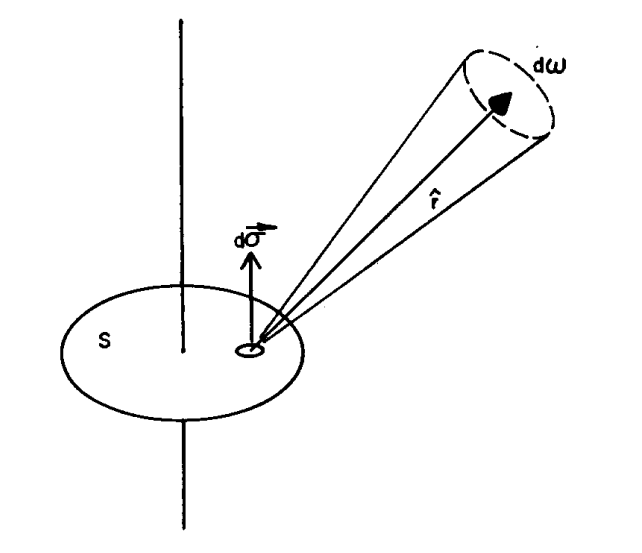
\includegraphics[width=.35\linewidth]{solidangle}
	\caption{Geometrical representation of a single plane detector \cite{Sullivan}.}
	\label{fig:planedetector}
\end{figure}
When performing a Monte Carlo simulation, the number of particles produced is large enough to consider one single particle as an infinitesimal $dN$, which is proportional to $dC=dGI$. It follows that
\begin{equation}\label{eq:dn}
dN \propto d\omega \cos\theta F(\omega)
\end{equation}
where $d\omega=d\varphi d\theta \sin\theta$, therefore from \eqref{eq:angD} and \eqref{eq:dn}, we have
\begin{equation}\label{eq:thetaMC}
dN \propto \cos^3\theta\sin\theta.
\end{equation}
Since $F$ does not depend on the azimuth angle, $\varphi$ is distributed according to a uniform distribution.

\subsection{Simulation procedure}

Muons crossing the scintillators can be generated starting from a \emph{seed event}, i.e. the coordinates $(x_0,y_0)$ of the muon impact point on the first scintillator surface and the angles $(\theta , \varphi)$ which define the muon direction.		
Impact point coordinates are uniformly generated $x \in [0,l]$ and $y \in [0,L]$, where $l = \SI{30}{cm}$ and $L = \SI{80}{cm}$ are the linear dimensions of the aligned scintillators.
The polar angle $\varphi$ is uniformly distributed in the range $\left[0,2\pi\right]$, whereas the zenith angle $\theta$ is generated in the range $\left[0,\pi/2\right]$ (i.e. the upper hemisphere) according to \eqref{eq:thetaMC}, by means of the \emph{try and catch} method.\\

The muons impact coordinates on the lower scintillator ($x^{'},y^{'}$) are computed from the seed event $\{x_0, y_0, \theta, \varphi \}$ according to

\begin{equation}
\begin{cases}
x^{'} = x_0 + r^{'} \sin \theta \cos \varphi   \\
y^{'} = y_0 + r^{'} \sin \theta \sin \varphi 
\end{cases}
\end{equation}

\noindent with
\begin{equation}
r^{'}= \frac{d}{\cos \theta}
\end{equation}
where $d$ is the distance between the upper scintillator (SC1) and the lower one (SC3)\footnote{Both in Section \ref{sec:geometric factor} calculations and in the Monte Carlo simulation, we have considered thick-less detectors. In the actual situation, with same dimensions aligned scintillators, a particle in the field of view of the telescope crosses the lower surface of the upper detector and the upper area of the lower one. Thus, $d$ will have to be measured according to this prescription.}.\\

The coincidence counts $N_{coinc}$ are given by events with $x^{'} \in [0,l]$ and $y^{'} \in [0,L]$, then we obtain the ratio of the number of muons which cross all the detectors to the total one $N_{tot}$ incident on the upper scintillator,

\begin{equation}
 g = \frac{N_{coinc}}{N_{tot}}.
\end{equation}

\begin{figure}[!htp]
	\centering
	\begin{subfigure}{.5\linewidth}
		\centering
		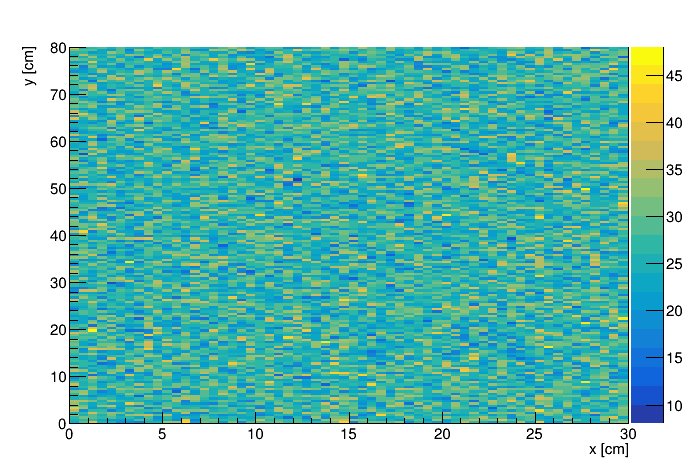
\includegraphics[width=\linewidth]{Scintillatore1}
		\caption{2D representation.}
	\end{subfigure}\hfill
	\begin{subfigure}{.5\linewidth}
		\centering
		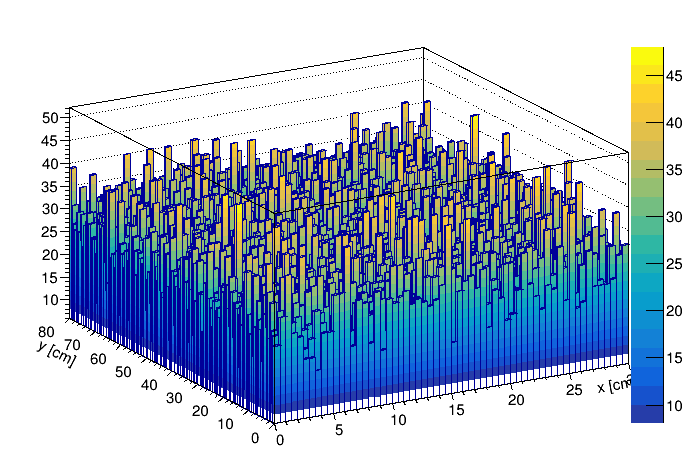
\includegraphics[width=\linewidth]{scintillatore13d}
		\caption{3D representation.}
	\end{subfigure}
	\caption{Generated muons distribution on the upper detector surface.}
	\label{fig:upper}	
\end{figure}
\begin{figure}[!htp]
	\centering
	\begin{subfigure}{.5\linewidth}
		\centering
		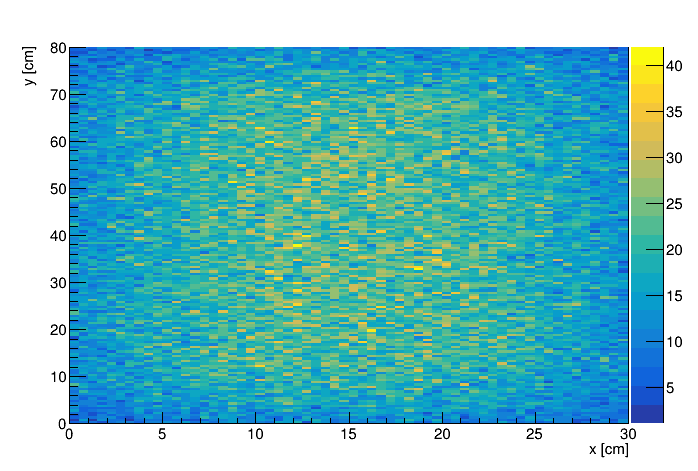
\includegraphics[width=\linewidth]{Scintillatore3}
		\caption{2D representation.}
	\end{subfigure}\hfill
	\begin{subfigure}{.5\linewidth}
		\centering
		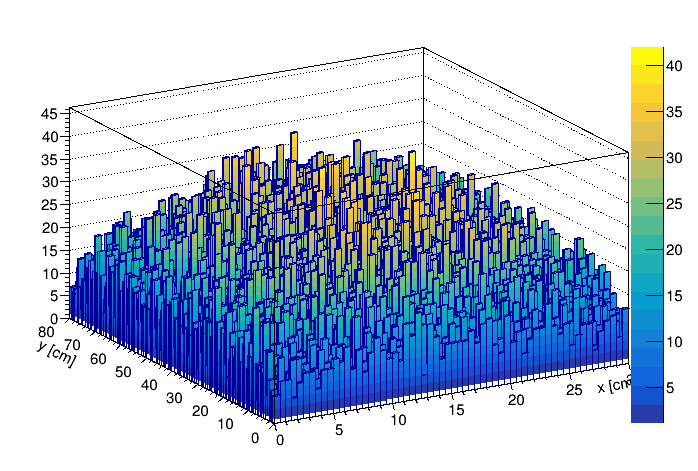
\includegraphics[width=\linewidth]{Scintillatore33d}
		\caption{3D representation.}
	\end{subfigure}
	\caption{Generated muons distribution on the lower detector surface.}
	\label{fig:lower}	
\end{figure}

The procedure is composed of $3500$ independent simulations and $250000$ muons have been generated in each of them. The spacial distributions of all generated muons on the surfaces of the upper and lower detectors are shown in Figure \ref{fig:upper} and \ref{fig:lower}. As expected, seed muons cover uniformly the surface of the upper scintillator, whereas the number of muons crossing the lower one show a decreasing trend at boundaries with respect to the internal area.
The distribution of the coefficient $g$, evaluated in each simulation, is fitted with a \emph{Gaussian}
\begin{equation}
\textrm{Gauss}(g;  \hat A , \hat g, \hat \sigma_{g})= \hat A e^{-\frac{(g -\hat g)^2}{2 {\hat \sigma_{g}}^2}}
\end{equation}
and the same procedure has been repeated twice: the first one refers to layouts displayed in Figure \ref{subfig:l1} and \ref{subfig:l2}, with an overall distance $d=\SI{8}{cm}$, whilst the second one refers to Figure \ref{subfig:l3} where $d=\SI{15}{cm}$. Fit results are shown in Figure \ref{fig:geom_eff}.

\begin{figure}[!htp]
	\centering
	\begin{subfigure}{.5\textwidth}
		\centering
		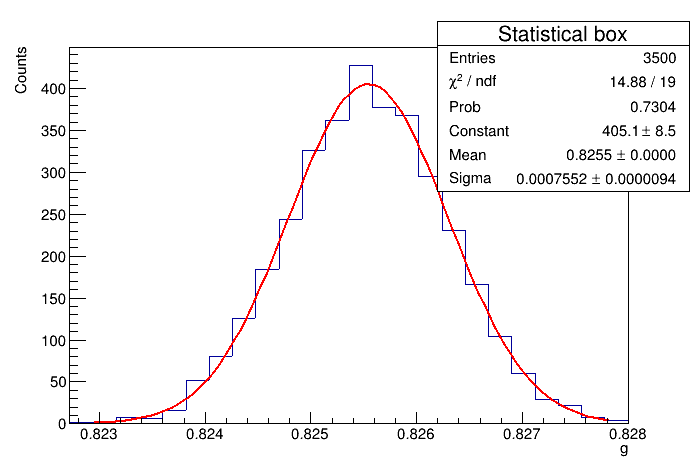
\includegraphics[width=\textwidth]{g_cerbero_up}
		\caption{Layout 1 and 2.}
	\end{subfigure}\hfill
	\begin{subfigure}{.5\textwidth}
		\centering
		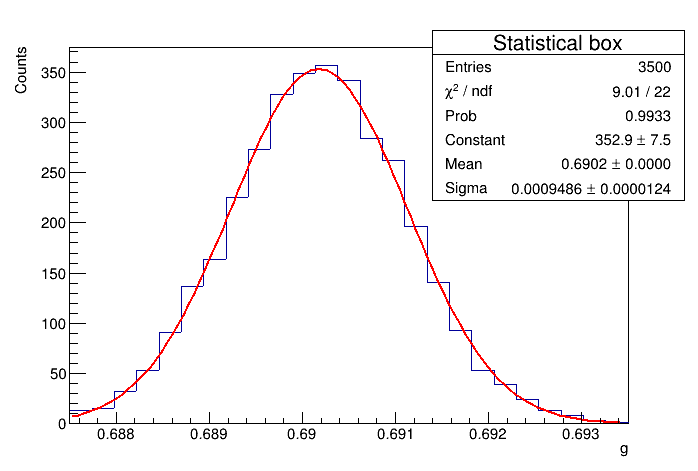
\includegraphics[width=\textwidth]{g_cerbero_middle}
		\caption{Layout 3.}
	\end{subfigure}
	\caption{Gaussian interpolation of the Monte Carlo results for the three layouts.}
	\label{fig:geom_eff}
\end{figure} 

\subsection{Comparison with analytical results}

Using $g$ we can rewrite Eq. \eqref{eq:intensity} as,
\begin{equation}\label{eq:g_Rozza}
	\begin{cases}
		I = C/\left(G_t \varepsilon_{t} \right)=S/\left(G_S \varepsilon_{s} \right)\\
		C = N_{double}/t \\
		S = N_{tot}/t
	\end{cases} \quad
	\Rightarrow\qquad \frac{C}{S} = \frac{N_{double}}{N_{tot}} \equiv g = \frac{G_t \varepsilon_{t}}{G_S \varepsilon_{s}}
\end{equation}
where $C$ and $S$ are the double and single counting rate respectively\footnote{For obvious reasons the time $t$ is the same in $C$ and $S$.}, $\varepsilon_{t}$ is the overall  efficiency of the particle telescope\footnote{See Section \ref{sec:geometric factor} for further details.} and $\varepsilon_{s}$ is the efficiency of the upper scintillator; $G_t$ and $G_S$ represent the geometric factor for the particle telescope and for the single detector, respectively. From the study made by Sullivan \cite{Sullivan} we know that the gathering power (i.e. the geometric factor) of a generic particle telescope is given by,
\begin{equation} \label{eq:gathering}
	\Gamma_F =\int_{\Omega}d\omega F(\omega)\int_{S}d\bm{\sigma}\cdot \mathbf{\hat{r}}
\end{equation}
where we remember that $F(\omega)$ represents the angular dependence of the radiation intensity. It follows that
\begin{equation}
	G_S = \int_{-X}^{X}\int_{-Y}^{Y}dxdy \int_{0}^{2\pi}d\phi \int_{0}^{1}\cos^3\theta d\left( \cos\theta\right) = 2\pi XY.
\end{equation}

Note that $X$ and $Y$ are half the length and width of the detector. Since all the scintillators have the same dimensions, we obtain $G_S = 0.3770\pm0.0006$ for all the detectors.\\
Finally, considering that $\varepsilon_{t} = \varepsilon_1 \varepsilon_3$ and $\varepsilon_{s} = \varepsilon_1$, we are able to estimate $g$, using the geometric factor of Eq. \eqref{eq:Thomas_simplified} and $G_S$ as reported below:
\begin{equation} \label{eq:G_MC}
	g = \frac{G_t\varepsilon_{t}}{G_S \varepsilon_{s}} = \frac{G_t \cdot \cancel \varepsilon_1\cdot \varepsilon_3}{G_S\cdot \cancel \varepsilon_1} = \frac{G_t}{G_S}\cdot \varepsilon_3
\end{equation}
Since the simulation procedure concern a purely geometrical effect, the efficiency of the detectors is assumed to be $1$ and \eqref{eq:G_MC} becomes
\begin{equation} \label{eq:G_MC_noeff}
	g = \frac{G_t}{G_S}
\end{equation}
hence, from \eqref{eq:G_MC_noeff} we can estimate $g$ and then compare it with the one obtained from the Monte Carlo. Results are reported in Table \ref{tab:G_t}.

\begin{table}[!htp]
	\centering
	\begin{tabular}{r|ccc}
		\toprule
		& $G_t/G_S$ & $\hat g$ & $p$-value\\
		\midrule
		Layout 1/2 & $0.825554\pm0.055870$ & $0.825544\pm0.000013$ & $0.9999$\\
		Layout 3 & $0.690180\pm0.051239$ & $0.690178\pm0.000016$ & $1.0000$\\
		\bottomrule
	\end{tabular}
	\caption{Accordance between $g=G_t/G_S$, given by the analytical calculation, and $\hat g$ estimated by means of the Monte Carlo method.}
	\label{tab:G_t}
\end{table}
In conclusion we can say the hypothesis made in the derivation of \eqref{eq:Thomas} in Section \ref{sec:geometric factor} are reasonable from the geometrical point of view due to the $p$-values largely above the adopted significance level equal to $0.05$.



\section{Uniformity studies}

\label{sec:uniformity_studies}

Subsequent to calculating the efficiency for each scintillator, a uniformity measurement of the latter is fundamental, in order to identify which portions of the detector work better or worse than the others. Further details will be explained in Section \ref{sec:uniformity}, nevertheless, the experimental layouts represented in Figure \ref{fig:uniformity} highlight the need to develop a Monte Carlo simulation.\\

In fact, when computing efficiency as
\begin{equation}
\varepsilon = \frac{N_{triple}}{N_{double}}
\end{equation}
\begin{figure}[!tbp]
	\centering
	\begin{subfigure}{.3\linewidth}
		\centering
		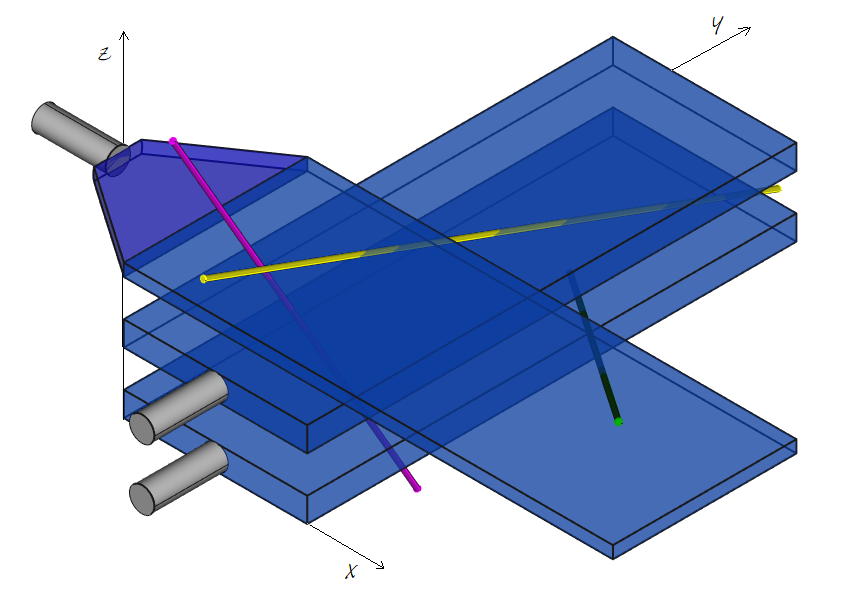
\includegraphics[width=\linewidth]{ParticlesMC}
		\caption{Axonometric projection.} 
		\label{subfig:particles}
	\end{subfigure}\hfill
	\begin{subfigure}{.3\linewidth}
		\centering
		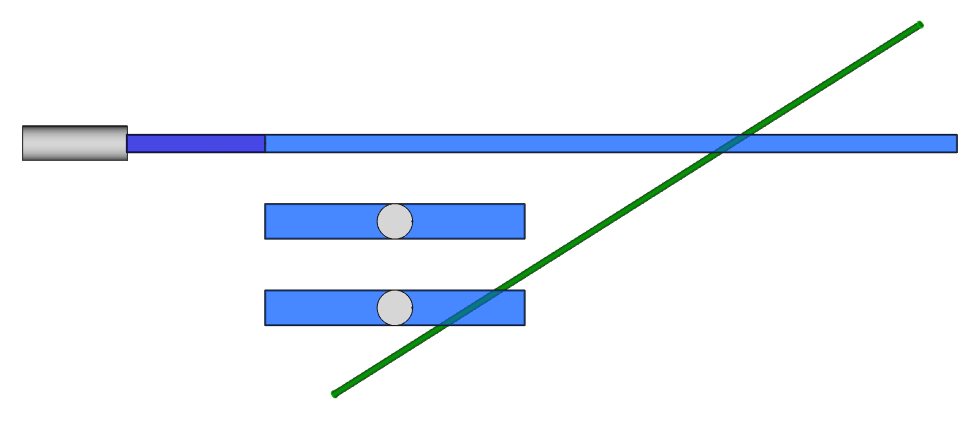
\includegraphics[width=\linewidth]{FalseDoppie_Lateral}
		\caption{Lateral view.} 
		\label{subfig:fd_lateral}
	\end{subfigure}\hfill
	\begin{subfigure}{.3\linewidth}
		\centering
		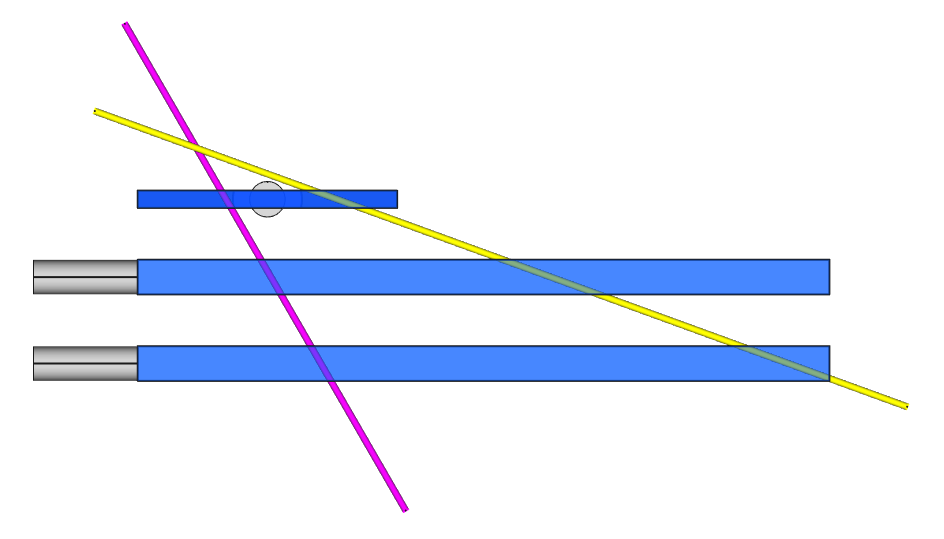
\includegraphics[width=\linewidth]{FalsaZona_Front}
		\caption{Front view.} 
		\label{subfig:fz_front}
	\end{subfigure}
	\caption{The purple particle is a true double, the yellow one contributes to a wrong area, whilst the green particle is a false double.} 
	\label{fig:uniformity_mc}
\end{figure}
the not-aligned geometry provides a systematic error that leads to an overestimate of $N_{double}$, thus an underestimated efficiency. The evidence of this behavior is clear from Figure \ref{fig:uniformity_mc}, where we can identify three event-types: $N_{double}^{t}$ as the true double counts (purple particle), $N_{double}^{wa}$ as the number of doubles referred to a wrong area (yellow particle) and $N_{double}^{f}$ as a false double count (since the middle-scintillator is not crossed by the green particle). With respect to the aligned geometry where the measured counts are $N_{double}=N_{double}^{t}$ and $N_{triple}=N_{triple}^{t}$, now
\begin{equation}\label{N_measured}
\left\{
\begin{array}{l}
N_{double}=N_{double}^{t}+N_{double}^{wa}+N_{double}^{f}\\\\
N_{triple}=N_{triple}^{t}+N_{triple}^{wa}
\end{array}
\right.
\end{equation}
therefore, if one define a \emph{wrong-area} efficiency\footnote{In $\varepsilon_{wa}$ formula \emph{double}/\emph{triple} subscripts have been omitted since the \emph{wrong-area} effect is purely geometric, thus it works both for \emph{triple} and \emph{double} counts in the same way.} as
\begin{equation}\label{eff_wa}
\varepsilon_{wa} = \frac{N^t}{N^t+N^{wa}}
\end{equation}
and a \emph{geometrical} efficiency as
\begin{equation}\label{eff_geom}
\varepsilon_{g} = \frac{N^t+N^{wa}}{N^t+N^{wa}+N^f}
\end{equation}
it is clear that from $N_{triple}^t=\varepsilon\cdot N_{double}^t$, \eqref{N_measured}, \eqref{eff_wa} and \eqref{eff_geom} follows that
\begin{equation}
\varepsilon_{wa}\cdot N_{triple} = \varepsilon\cdot\varepsilon_{wa}\cdot\varepsilon_g\cdot N_{double}
\end{equation}
thus, the efficiency $\varepsilon$ of the middle-scintillator (due to radiation-matter interaction) is given by
\begin{equation}\label{eq:eff_correct}
\varepsilon = \frac{N_{triple}}{\varepsilon_g\cdot N_{double}}
\end{equation}
The main purpose of the following Monte Carlo procedure is the simulation of the explained geometrical effect and an estimation of the weight defined in \eqref{eff_geom}, needed as a correction on the measured double counts.

\subsection{Simulation procedure}
The implemented solution is based on the generation of $M$ muons in the volume of the upper detector, i.e. we have four uniformly distributed random numbers $x_1\in\left[0, L\right]$, $y_1\in\left[0, l\right]$, $z_1\in\left[z_1^{d},z_1^{u}\right]$ and $\varphi\in\left[0, 2\pi\right]$, where $L$, $l$ are the scintillators length and width, respectively, $z_1^{d/u}$ are the $z$-coordinates of the lower/upper surface of the detector and $\varphi$ is the azimutal angle. Finally the zenith angle $\theta\in\left[0, \pi/2\right]$ is generated following \eqref{eq:thetaMC} distribution by means of what is known as \emph{try and catch} method. Since we deal with MIPs, one can reasonably neglect their deflection (following interaction with detectors) and describe their trajectory by making use of straight line equations
\begin{equation}\label{eq:straight}
\left\{
\begin{array}{l}
x = x_1 + t\cdot\sin\theta\cos\varphi\\\\
y = y_1 + t\cdot\sin\theta\sin\varphi\\\\
z = z_1 + t\cdot\cos\theta
\end{array}
\right.
\end{equation}
From \eqref{eq:straight} it follows that
\begin{equation}
\left\{
\begin{array}{l}
x = \textrm{fixed}\\\\
y = y_1 + (x-x_1)\cdot\tan\varphi\\\\
z = z_1 + (x-x_1)\cdot\displaystyle\frac{1}{\tan\theta\cos\varphi}
\end{array}
\right.
\end{equation}
then
\begin{equation}
\left\{
\begin{array}{l}
x = x_1 + (y-y_1)\cdot\displaystyle\frac{1}{\tan\varphi}\\\\
y = \textrm{fixed}\\\\
z = z_1 + (y-y_1)\cdot\displaystyle\frac{1}{\tan\theta\sin\varphi}
\end{array}
\right.
\end{equation}
and
\begin{equation}
\left\{
\begin{array}{l}
x = x_1 + (z-z_1)\cdot\tan\theta\cos\varphi\\\\
y = y_1 + (z-z_1)\cdot\tan\theta\sin\varphi\\\\
z = \textrm{fixed}
\end{array}
\right.
\end{equation}

Due to non-negligible scintillators height, the simulation procedure recognizes that a muon crosses the middle detector\footnote{The case of particles crossing the middle scintillator without passing through its surfaces is excluded by the simulation, since of course they could not cross the lower detector, which is aligned with the middle one.} if it passes through the lower or upper surface. Instead, concerning the lower detector, it can be crossed by a particle even in the lateral areas without involving upper or lower surfaces.\\

Now we can define a boolean variable $sc_i$ which is \emph{true} if the particle crosses the $i$-scintillator, otherwise it is \emph{false}, and two additional variables $sc_2^a$ and $sc_2^{wa}$ which are referred to the correct and wrong area of the middle detector, respectively. As a consequence, events are classified in the following way:
\begin{equation}
\begin{array}{l}
sc_1 \,\wedge\, sc_2^a \,\wedge\, sc_3 \qquad \Rightarrow \qquad N_{double}^t\\\\
sc_1 \,\wedge\, sc_2^{wa} \,\wedge\, sc_3 \qquad \Rightarrow \qquad N_{double}^{wa}\\\\
sc_1 \,\wedge\, \textrm{\texttt{not}} \left(sc_2^a \vee sc_2^{wa}\right) \,\wedge\, sc_3 \qquad \Rightarrow \qquad N_{double}^f
\end{array}
\end{equation}
hence, the geometrical efficiency is calculated according to \eqref{eff_geom}. The described procedure is repeated $N_{MC}$ times, in order to reduce the statistical error, and an histogram of $\varepsilon_{g}$ is produced. The details of the developed \texttt{C++} functions are reported in Appendix \ref{app:eff_geom_MC}.\\

\begin{table}[!hbp]
	\centering
	\begin{tabular}{cc}
	\toprule
	Variable & Value ($\si{\centi\meter}$)\\
	\midrule
	$L$ & $80.0$\\
	$l$ & $30.0$\\
	$h_1$ & $1.0$\\
	$h_2$ & $3.8$\\
	$h_3$ & $3.8$\\
	$d_1$ & $2.5$\\
	$d_2$ & $2.0$\\
	\bottomrule
	&\\
	\multicolumn{2}{c}{\footnotesize (a) \emph{Caronte - Minosse}}
	\end{tabular}\qquad\qquad
	\begin{tabular}{cc}
		\toprule
		Variable & Value ($\si{\centi\meter}$)\\
		\midrule
		$L$ & $80.0$\\
		$l$ & $30.0$\\
		$h_1$ & $3.8$\\
		$h_2$ & $1.0$\\
		$h_3$ & $3.8$\\
		$d_1$ & $7.0$\\
		$d_2$ & $7.0$\\
		\bottomrule
		&\\
		\multicolumn{2}{c}{\footnotesize (b) \emph{Cerbero}}
	\end{tabular}
	\caption{Geometrical parameters of the detectors setup. $h_{1/2/3}$ represents the height of the upper/middle/lower scintillator, while $d_1$, $d_2$ are the distances between the upper and the middle detector and between the middle and the lower one, respectively.} \label{tab:length}
\end{table}

Each length parameter has been measured by means of a meter-stick: measurements are summed up in Table \ref{tab:length}.
\begin{figure}[!htp]
	\centering
	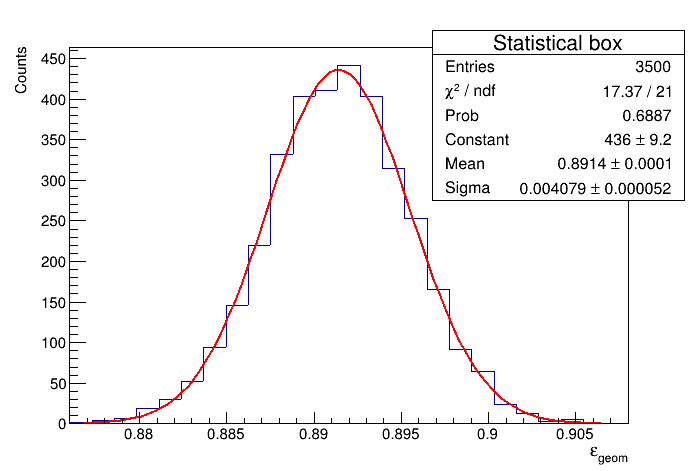
\includegraphics[width=.7\linewidth]{eff_geom_MC}
	\caption{Geometrical efficiency distribution.} 
	\label{fig:mc_eff_g}
\end{figure}
Figure \ref{fig:mc_eff_g} shows a resulting histogram referred to \emph{Caronte - Minosse} layout 3, with $M=250000$ and $N_{MC}=3500$, fitted with a \emph{Gaussian} distribution\footnote{With respect to the statistical box of Figure \ref{fig:mc_eff_g}, calling Constant $=C$, Mean $=\langle\varepsilon_{g}\rangle$ and Sigma $=\sigma$, the Gaussian distribution is $G(\varepsilon_{g})=C\cdot \exp\left(- \left(\varepsilon_{g}- \langle\varepsilon_{g}\rangle\right)^2/\left(2\sigma^2\right)\right)$.}, as expected by considering the \emph{central limit theorem}. The correspondence between simulated efficiencies and the Gaussian fit-function is clear, since
\begin{equation}
P_{21}\left(\chi^2 \geq \chi^2_{obs} \right) = 68.87\,\%
\end{equation}
where $21$ is the number of degrees of freedom and $\chi^2_{obs}$ is the observed $\chi^2$-value.\\

Finally, simulated geometrical efficiencies for each layout (with respect to Figure \ref{fig:uniformity}) are summed up in Table \ref{tab:all-effg}.

\begin{table}[!hbp]
	\centering
	\begin{tabular}{r|cc}
	\toprule
	&\emph{Caronte - Minosse} & \emph{Cerbero}\\
	\midrule
	Layout 1 & $0.939748$ & $0.905542$\\
	Layout 2 & $0.938381$ & $0.903697$\\ 
	Layout 3 & $0.891402$ & $0.850164$\\
	\bottomrule
	\end{tabular}
	\caption{Simulated geometrical efficiencies.}\label{tab:all-effg}
\end{table}

\subsection{Uncertainty estimation}

As discussed above, the main purpose of this Monte Carlo simulation is to estimate $\varepsilon_{g}$ which leads to the rejection of geometrical systematic error, but the procedure itself is affected by an error we want to keep track of.\\

A source of error on $\varepsilon_{g}$ is given by the uncertainty on the measured geometrical parameters $\pi_j$ that enter in the simulation, thus the geometrical efficiency is estimated several times by varying these parameters in the range $\left[\pi_j-\sigma_{\pi_{j}}, \pi_j+\sigma_{\pi_{j}} \right]$. Therefore, the uncertainty on $\varepsilon_{g}$ is empirically determined as the maximum deviation from the mean efficiency $\langle\varepsilon_{g}\rangle$.\\
\begin{equation}
\sigma_{\varepsilon_{g}}=\max_k\left|\varepsilon_{g_k}  -\langle\varepsilon_{g}\rangle\right|
\end{equation}
where $k=1, ..., 3^J$ and $J$ is the number of parameters $\pi_j$.\\

The computational cost of this method grows exponentially, for this reason it is worth restricting the analysis only on variables affected by the higher uncertainties. $L,l, h_i$ are given by the manufacturer, hence the most relevant errors are on the distances $d_1$ and $d_2$ between detectors: $\sigma_d=\SI{0.5}{cm}$ is assumed for both $d_1$ and $d_2$ as a reasonable upper limit, in order to evaluate the impact of a change of their central values on the estimated $\varepsilon_{g}$. Table \ref{tab:err-effg} shows the results.

\begin{table}[!hbp]
	\centering
	\begin{tabular}{r|cc}
		\toprule
		&\emph{Caronte - Minosse} & \emph{Cerbero}\\
		\midrule
		Layout 1  & $0.940\pm 0.005$ & $0.906\pm 0.005$\\
		Layout 2 & $0.938\pm 0.005$ & $0.904\pm 0.005$\\ 
		Layout 3 & $0.892\pm 0.009$ & $0.850\pm 0.008$\\
		\bottomrule
	\end{tabular}
	\caption{Simulated geometrical efficiencies, errors estimation included.}\label{tab:err-effg}
\end{table}



\chapter{Instrumentation characterization}
Before performing physics measurements, a detailed characterization of both scintillators and electronics modules is necessary, in order to identify possible systematic uncertainty sources then employ reasonable corrections to measures afterward. Moreover, further reasons to fully benefit from this investigation are certainly given by the need to choose an optimized setup of the instrumentation and by the importance of comprehending instruments responses.

\section{Electronics modules characterization}
\subsection{Discriminator} \label{discriminator}
The first module (not incorporated in the detector structure) involved in pulse processing is the discriminator whose input is a linear pulse, while its output is a logic pulse. Among several kinds of triggering, a \emph{leading edge} one has been used, so that the logic pulse is provided when the input exceeds a fixed discrimination level.\\

In particular a \textbf{CAEN N.147 8-Channel Low-Threshold Discriminator} (see Appendix \ref{app:discriminator}) has been employed: 7 of 8 channels have been studied (as the last channel was damaged) by means of a square-pulses generator, in order to determine possible shifts between threshold values measured with a tester and the actual ones, inferred by sending to the channel-input a series of different amplitude pulses. The procedure provides for a gradual increase of the input amplitude up to the first value that corresponds to a non-flat output: that value is the experimental threshold voltage. This process has been repeated for several thresholds\footnote{The trigger level is adjustable by turning a screw.}: no relevant differences between tester values and experimental threshold levels have been observed (up to electronics noise fluctuations).\\

The discriminator gives also the possibility to vary the output duration (by turning a specific screw) and this feature turns out to be fundamental in avoiding a not-negligible source of systematic errors (see Subsection \ref{sub:detection_eff}).
\begin{figure}[!htp]
	\centering
	\begin{subfigure}{.3\linewidth}
		\centering
		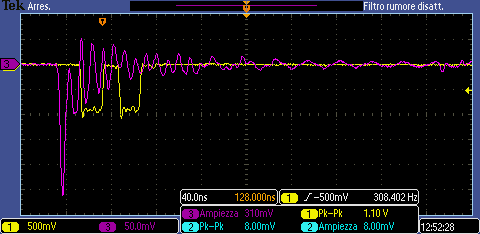
\includegraphics[width=\linewidth]{characterization/double}
		\caption{Wrong double output generation.}
		\label{subfig:double}
	\end{subfigure}\hfill
	\begin{subfigure}{.3\linewidth}
		\centering
		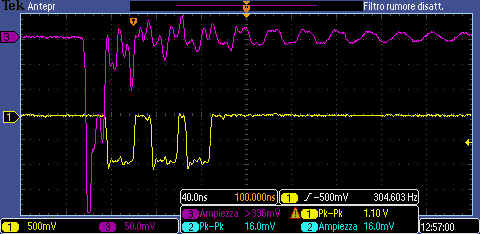
\includegraphics[width=\linewidth]{characterization/triple}
		\caption{Wrong triple output generation.}
		\label{subfig:triple}
	\end{subfigure}\hfill
	\begin{subfigure}{.3\linewidth}
		\centering
		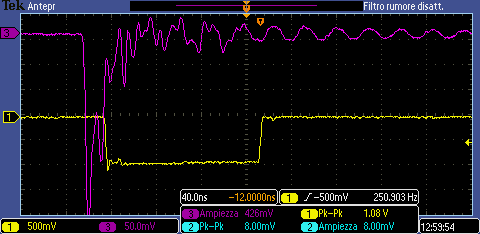
\includegraphics[width=\linewidth]{characterization/single}
		\caption{Correct single output generation.}
		\label{subfig:single}
	\end{subfigure}
	\caption{Oscilloscope visualization. The purple lines represents \emph{Cerbero} anodic outputs, while the yellow ones are the logic pulses provided by the discriminator.}
	\label{fig:window}
\end{figure}
Problems arise when a quite low trigger voltage is combined with an input pulse affected by an important noise level: one is able to note by observing Figures \ref{subfig:double} and \ref{subfig:triple} how this situation could lead to the generation of more than one output pulses per single input, due to a too small time-window. This behavior certainly represents a problem when counting experiments are carried out. Since the discriminator is not able to provide a new pulse when the previous one is still ongoing, the problem is satisfactorily solved by widening the time-window up to the typical duration of the input signal (Figure \ref{subfig:single}).

This kind of issue has not been observed in the less noisy \emph{Minosse} and \emph{Caronte} detectors, but, as a preventive action, the corresponding discriminator outputs duration is set according to what explained above.

\begin{table}[!htp]
	\centering
	\begin{tabular}{cc}
		\toprule
		Detector	&	Time-window $(\si{\nano\second})$ \\
		\midrule
		\emph{Caronte}	&	$40$ \\
		\emph{Cerbero}	&	$80$ \\
		\emph{Minosse}	&	$40$ \\
		\bottomrule		
	\end{tabular}
	\caption{Discriminator output time-windows.}
	\label{window}
\end{table}

A side effect of a larger time-window is the growth of the measure dead-time, but this does not create a problem in muons lifetime measurements. As a matter of fact the expected cosmic muons rate at the ground\footnote{According to \eqref{mu-rate} the expected muon rate per surface unit at the ground is equal to $\approx 1\,\si{cm^{-2}} \,\si{min^{-1}}$ (for a thin horizontal detector), which provides a rate of about $\SI{40}{\hertz}$ relative to the involved detectors.} is $\approx \SI{40}{\hertz}$: this means that two consecutive muons are averagely time-separated by
\begin{displaymath}
\langle t \rangle  = \frac{1}{\langle \Gamma \rangle} \approx \frac{1}{\SI{40}{\hertz}}=2.5\cdot 10^7\,\si{\nano\second}\gg \SI{80}{\nano\second}.
\end{displaymath}

\subsection{Delay unit}
When configuring the electronic chain setup, the delays between different signals have to be kept under control, for the purpose of a correct pulse processing: this goal is achieved by employing LEMO cables of suitable lengths and/or using a delay unit. The latter is a passive module as it do not need a power supply, therefore the delay is realized in a very simple way, by letting the signal pass through internal cables from input to output.\\

The matter is to verify to what extent the nominal delay matches the experimental one.  
\begin{figure}[!h]
	\centering
	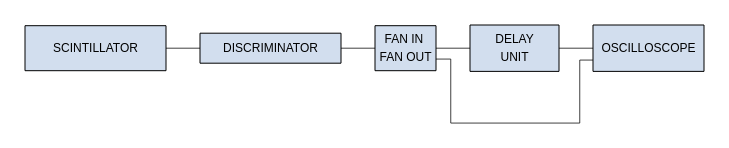
\includegraphics[width=.8\linewidth]{characterization/delay}
	\caption{Configuration employed during delay unit characterization.}
	\label{fig:delay}
\end{figure}
The setup in Figure \ref{fig:delay} shows how the delay can be directly observed measured. Although one could measure by means of oscilloscope's cursors the input/output phase shift induced by \textbf{CAEN N. 108 Dual Delay}, a more systematic approach\footnote{The waveforms have not been observed to be static, instead they are subject to small fluctuations, thus several signals have been acquired.} has been preferred. Both input and output waveforms are displayed in an oscilloscope and acquired (15 for each nominal delay) so as to perform offline analyses.
\begin{figure}[!h]
	\centering
	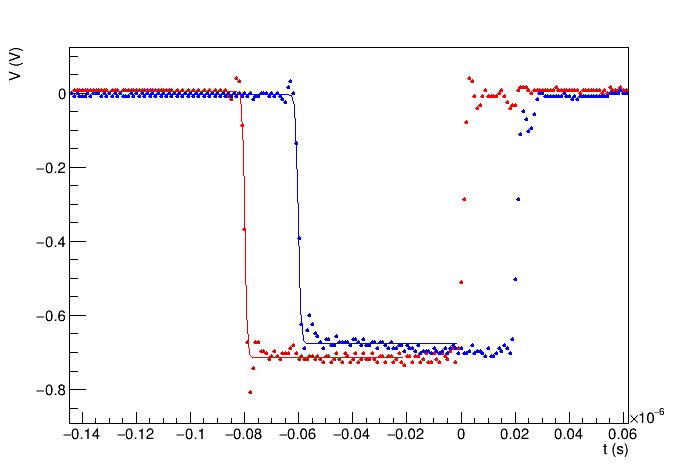
\includegraphics[width=.75\linewidth]{characterization/FD_20ns}
	\caption{Input (red) and output (blue) waveforms corresponding to $\SI{20}{\nano\second}$ nominal delay.}
	\label{fig:wf}
\end{figure}
Most difficulties are given by the limited sampling rate $(\SI{1}{\giga\hertz})$, compared with the rise-time of the square pulses (see Figure \ref{fig:wf} for instance), then, in order to use a reasonable number of points, waveforms are fitted with \emph{Fermi-Dirac}-like functions
\begin{equation} \label{eq:FD}
V(t)=\frac{\alpha}{1+e^{\beta\left(t-\gamma\right)}}+\delta
\end{equation}
where $\alpha,\beta,\gamma,\delta$ are parameters. \eqref{eq:FD} is then inverted
\begin{equation}
t(V) = \frac{1}{\beta}\cdot\ln\left(\displaystyle\frac{\alpha}{V-\delta}-1  \right)+\gamma
\end{equation}
and the experimental delay $\Delta t_{exp}$ is determined as
\begin{equation}
\Delta t_{exp} = t_{blue}(\SI{-0.36}{V})-t_{red}(\SI{-0.36}{V}).
\end{equation}

The measure is repeated $15$ times, then the mean value is computed and a graph of experimental delays versus the nominal ones is finally built. Figure \ref{fig:delaylinearity} points have been fitted with a linear function
\begin{equation}\label{eq:linear}
y=A+Bx
\end{equation}
where $x$ and $y$ represents the nominal and experimental delay, respectively.
\begin{figure}[!htp]
	\centering
	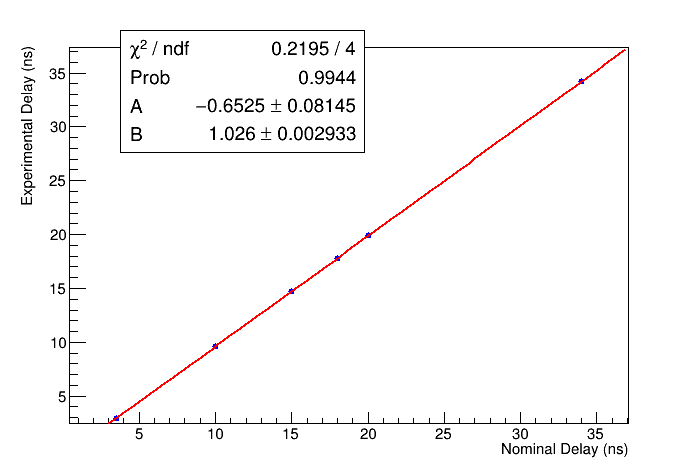
\includegraphics[width=.75\linewidth]{characterization/DelayLinearity}
	\caption{Relation between the nominal delay and experimental one. Error bars are calculated as the standard deviation of the $15$ measures (for each delay). Notwithstanding they are drawn, they are not visible due to their smallness.} \label{fig:delaylinearity}
\end{figure}
The accordance between data and the model \eqref{eq:linear} is excellent since
\begin{equation}
P_4\left(\chi^2\geq\chi_{obs}^2\right)=99.44\,\%
\end{equation}
but the fit results highlight a discrepancy with the ideal behavior $A_{id}=0$ and $B_{id}=1$ of order $8\sigma_A$ and $9\sigma_B$, respectively. Therefore, in the next analyses a correction to nominal delays due to a systematic error is mandatory:
\begin{equation} \label{correction}
\Delta t_{real} = A + B\cdot\Delta t_{nom}
\end{equation}
with
\begin{equation}
A=\left(-0.65\pm 0.08\right)\,\si{\nano\second}\qquad\quad B=\left(1.026\pm 0.003\right)
\end{equation}
The covariance matrix is
\begin{equation}
\textrm{C}_{AB}=\left(
\begin{array}{cc}
0.00663 & -0.00022\\\\
-0.00022 & 8.6\cdot 10^{-6}
\end{array}
\right).
\end{equation}

To conclude, from errors propagation formula, the uncertainty on $\Delta t_{real}$ will depend on the nominal delay in accordance with
\begin{equation} \label{err_correction}
\sigma_{\Delta t_{real}} = \sqrt{\sigma_A^2 + \left(\Delta t_{nom} \cdot \sigma_B\right)^2 + 2\Delta t_{nom}\cdot\sigma_{AB}  }.
\end{equation}

\subsection{Logic unit}
The programmable logic unit is a module used to make boolean operations between signals and it is employed in our experiment to perform coincidences between signals.
When configuring the electronics setup for the measurement of the muon lifetime, logic unit modules will be employed in order to perform start and stop topologies for the $\mu$ decay triggering. For this reason the characterization of the logic unit response is mandatory.

The logic unit is programmed in $\texttt{AND}$ mode in order to perform coincidences between signals. Therefore two NIM signals entering the 4-fold logic unit produce an output signal only if they are overlapped within a few ns.
Therefore, the aim of the logic unit characterization is to quantify the maximum time separation between two signals such that their overlapping is not enough to succeed in performing an $\texttt{AND}$ operation.\\

The characterization setup is shown in Figure \ref{logic_unit_1scinti}.
The pulse that is coming from the anode, if above the discriminator threshold, is divided along three different lines by means of a Fan-In/Fan-Out module.
One signal goes directly to a counter, which measures the total number of counts $N_{tot}$ for each measurement. 
The other two signals reach the logic unit along two different lines, i.e. passing through a delay unit or not. Finally the output signal of the logic unit is sent to a different channel of the counter, which counts the number of coincidences $N_{coinc}$ between the signals passing through the two lines, one delayed respect to the other.
In this configuration it is clear that, by means of the delay unit, one of the signal can be easily displaced in time. As a matter of fact, the measured value for $N_{coinc}$ depends on the delay which can be increased until the time separation among signals guarantees an overlapping sufficient to produce an output pulse. If the time shift becomes too large they are not recognized as overlapped anymore, consequently, since the two signals are not logically summed, the number of coincidences recorded at the counter changes abruptly.


\begin{figure}[!h]
	\centering
	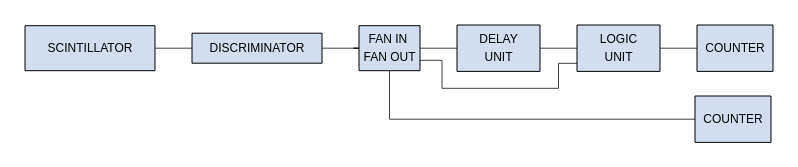
\includegraphics[width=\linewidth]{characterization/logic_unit_1scinti}
	\caption{Configuration employed during logic unit characterization with one scintillator.}
	\label{logic_unit_1scinti}
\end{figure}

The maximum time separation between coincident signals can be quantified comparing to what extent the counts measured in the two channels of the counter change when the delay is increased.
Therefore we can study the ratio between coincidences and total event counts as a function of the delay $\Delta t$ set on the delay unit, i.e.
\begin{equation} \label{eq:fermi_dirac}
f(\Delta t) = \frac{N_{coinc}(\Delta t)}{N_{tot}} .
\end{equation}

The sharp decreasing of the counts when the delay is increased can be parameterized by an empirical \emph{Fermi-Dirac}-like function which is used to perform the fit
\begin{equation} \label{eq:fermidirac}
f(\Delta t) = \frac{f_0}{1 + e^{k(\Delta t- t_0)}}
\end{equation}
where $f_0$ is the left-side asymptotic value of $f(\Delta t)$ for small $\Delta t$, $k$ is a constant and $t_0$ is the time at which $f(t_0) = 0.5 f_0$. As a matter of fact, the parameter $t_0$ corresponds to the discriminator output signal time-window (see Section \ref{discriminator}).\\

The width of the $f(t)$ distribution can be approximated from the tangent line to $f(t)$ evaluated at the point $t_0$
\begin{equation}
y(t) = - \frac{f_0}{4} k t + \frac{f_0}{2} \left(1 + \frac{k t_0}{2}\right)
\end{equation}
computing the distance between $t_0$ and the point $t^*$ at which the tangent line intersects the abscissa. $t^*$ is given by
\begin{equation}
t^* = \frac{2}{k} \left(1 + k \frac{t_0}{2}\right) .
\end{equation}
therefore the maximum time width $\delta_{T}$ of the logic unit within two signals are logically summed in $\texttt{AND}$ mode can be evaluated from the fit parameters as
\begin{equation}
\delta_{T} = 2 ( t^* - t_0 ) =  \frac{4}{k}.
\end{equation}

In order to reduce the systematic uncertainties, the real value of the delay with respect to the nominal one and its corresponding uncertainty have been computed by means of \eqref{correction} and \eqref{err_correction}, determined in the characterization of the delay unit.
Figure \ref{fig:fit_1scinti} shows the resulting fit of \eqref{eq:fermidirac} to the collected dataset. 
\begin{figure}[!htp]
	\centering
	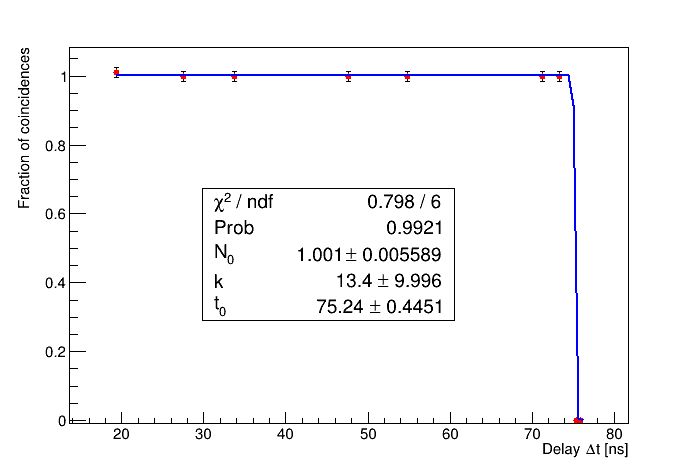
\includegraphics[width=.75\linewidth]{characterization/LogicUnit1}
	\caption{Logic unit characterization with a single split signal.} \label{fig:fit_1scinti}
\end{figure}
The estimated parameters are
\begin{equation}
\begin{array}{l}
f_0 = 1.001 \pm 0.006 \\
k = ( 13.397 \pm 9.996 ) \,  \si{ns^{-1}} \\
t_0 = ( 75.24 \pm 0.45 ) \,  \si{ns} .
\end{array}
\end{equation}
and the covariance matrix is
\begin{equation}
\textrm{C}=\left(
\begin{array}{ccc}
     3.12 \cdot 10^{-5}  &  5.19 \cdot 10^{-5}  &  2.38 \cdot 10^{-7} \\
    5.19 \cdot 10^{-5} &      99.93   &      4.27\\
    2.38 \cdot 10^{-7}  &       4.27   &    0.198
\end{array}
\right)
\end{equation}

The accordance between data and the model \eqref{eq:fermi_dirac} is excellent since
$P_6\left(\chi^2\geq\chi_{obs}^2\right)=99.21\,\%$.
It can be observed that the counts fall quite sharply around $\SI{75.2}{ns}$ and almost no counts are registered for delays greater than this.
The time width of the logic unit obtained is:
\begin{equation}
\delta_T = ( 0.299 \pm 0.223) \, \si{ns}
\end{equation}

The relative uncertainty obtained on $\delta_T$ is quite big $\left( \delta_{\delta_T} / \delta_T \sim 74.6 \%\right)$ since delay small enough to sample the step decreasing of the function were not experimentally found.\\

Almost the same strategy can be applied with two scintillators. 
The characterization setup is shown in Figure \ref{logic_unit_1scinti}:
\begin{figure}[!h]
	\centering
	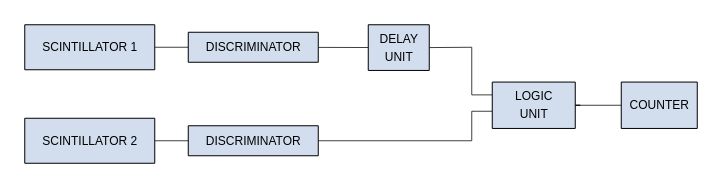
\includegraphics[width=\linewidth]{characterization/logic_unit_2scinti}
	\caption{Configuration employed during logic unit characterization with two scintillators.}
	\label{logic_unit_2scinti}
\end{figure}
in this configuration the signals come from two different scintillators and, before reaching the logic unit, one of them can be delayed with respect to the other by means of the delay module. Similarly, we can study the decreasing in the number of counts of coincident signals $N_{coinc}$ when the delay is increased.
The decreasing of the counts is parameterized by the empirical function
\begin{equation} \label{eq:fermi_dirac_1}
N_{coinc}(\Delta t) = \frac{N_0}{1 + e^{k(\Delta t- t_0)}}
\end{equation}
which is used to perform the fit.
Figure \ref{fig:fit_2scinti} shows the resulting fit of \eqref{eq:fermi_dirac_1} to the collected dataset. 
\begin{figure}[!htp]
	\centering
	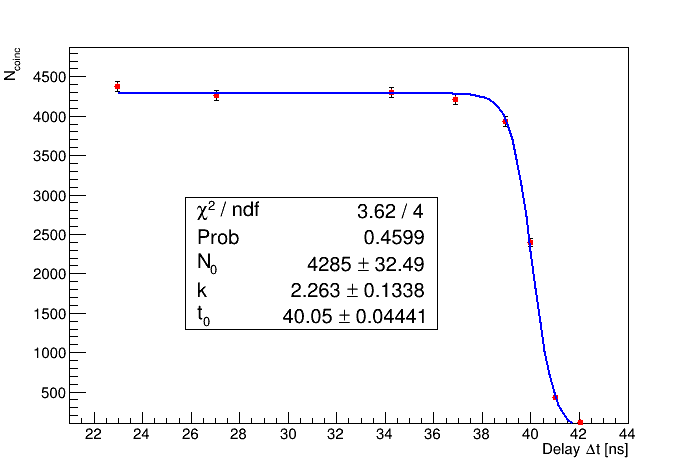
\includegraphics[width=.75\linewidth]{characterization/LogicUnit2}
	\caption{Logic unit characterization with signals from two scintillators.} \label{fig:fit_2scinti}
\end{figure}
The parameters estimated from the fit are
\begin{equation}
\begin{array}{l}
N_0 = ( 4.285 \pm 0.032 ) \cdot 10^3 \\
k = ( 2.26 \pm 0.13 ) \,  \si{ns^{-1}} \\
t_0 = ( 40.0514 \pm 0.044 ) \,  \si{ns}
\end{array}
\end{equation}

\noindent The covariance matrix is
\begin{equation}
\textrm{C}=\left(
\begin{array}{ccc}
1055.28  &     -1.22    &   -0.447 \\
-1.22   &     0.018   &    0.0017 \\
-0.447   &    0.0017  &     0.0019 \\
\end{array}
\right)
\end{equation}

The accordance between data and the model \eqref{eq:fermi_dirac_1} is satisfactory since
$P_4\left(\chi^2\geq\chi_{obs}^2\right)=45.98\,\%$.
The time width of the logic unit obtained is
\begin{equation}
\delta_T = ( 1.77 \pm 0.10 ) \, \si{ns}.
\end{equation}

The uncertainty on the measured value is quite small ($\delta_{\delta_T} / \delta_T \sim 6 \%$) since the fall in the number of counts is less abrupt and more data have been sampled in this region.
The different value for the estimated parameter $t_0$ in the two characterization schemes employed is simply due to a different choice of the discriminator channel, whose time-window are given in Table \ref{window}.
Moreover, when dealing with two scintillators, casual coincidences must be taken into account. The chance coincidence rate from uncorrelated input at rates $R_1$ and $R_2$ (i.e. event rates in the two scintillators)  is:
\begin{equation}
R_{chance} =  \tau R_1 R_2 \, \cite{Knoll}
\end{equation}
where $\tau$ is the time-window ($\tau = \SI{40}{ns}$). Here $R_1 = R_2 = \SI{40}{Hz}$ (see Section \ref{discriminator}), which gives $R_{chance} < 10^{-4}\si{Hz}$, which is negligible. 
Furthermore the decreasing of the number of counts is less abrupt since the signals come from two different scintillators, hence the effects of time jitter and amplitude walk become more important.

\subsection{Coincidence unit}
\documentclass[a4paper, 12pt]{report}
\usepackage{graphicx}

\begin{document}
	
\section{Electronics Modules Characterization}
\subsection{Coincidence Unit}
As the logic unit, the coincidence unit is a module used to make boolean operations between signals . The coincidence unit's imputs are logic pulses and the outputs are logic pulses if pulses appear at all imputs within a time interval (resolving time). In our experiment it is used(as the logic unit) to perform coincidences between signals.\\

The same approach used with the characterization of the logic unit can be applied to the coincidence unit.


The characterization setup is shown in Figure \ref{coinc_unit} and it is equivalent to the first set up for the logic unit . 

\begin{figure}[!h]
	\centering
	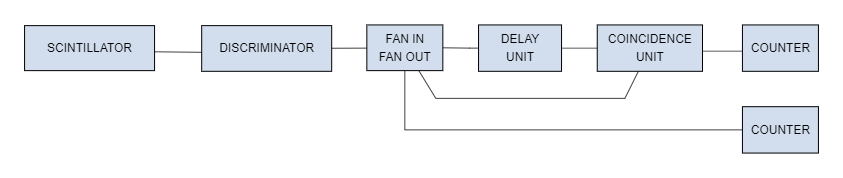
\includegraphics[width=\linewidth]{coinc_unit.png}
	\caption{Configuration employed during coincidence unit characterization}
	\label{coinc_unit}
\end{figure}


Also the fitting function(\eqref{eq:fermidirac}) and the way in which the errors are calculated are  always the same of the first characterization of the logic unit,thus the results can be shown directly. 


The estimated parameters are
\begin{eqnarray}
f_0 = 0.995 \pm 0.005\\
k = ( 20.936 \pm 9.790 ) \,  \si{ns^{-1}} \\
t_0 = ( 38.100 \pm 0.112 ) \,  \si{ns} .
\end{eqnarray}
and the covariance matrix is
\begin{equation}
\textrm{C}=\left(
\begin{array}{ccc}
     2.24 \cdot 10^{-5}  &  -1.39\cdot 10^{-2} &  -1.59 \cdot 10^{-4} \\
    -1.39 \cdot 10^{-2} &      95.84  &      0.98\\
    -1.59\cdot 10^{-4}  &       0.98   &    1.26\cdot 10^{-2} 
\end{array}
\right)
\end{equation}



The accordance between data and the model is excellent since $P_8\left(\chi^2\geq\chi_{obs}^2\right)=99.96\,\%$.
As in the  characterization of the logic unit it can be observed that  the counts fall quite sharply around a value of  delay and almost no counts are registered for delays greater than this.  
The value of this delay is almost \SI{38.1}{ns} and the time width of the coincidence unit obtained is: 

\begin{equation}
\delta_T = ( 0.191\pm 0.089 ) \, \si{ns}.
\end{equation}

The relative uncertainty obtained on $\delta_T$ is quite big $\left( \delta_{\delta_T} / \delta_T \sim 46.6 \%\right)$ since the decrease of the function is steep thus few data have been sampled in this region.   \\

\begin{figure}[!h]
	\centering
	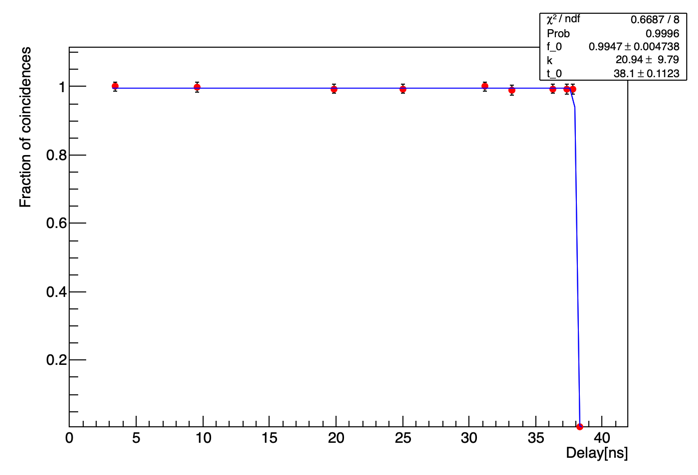
\includegraphics[width=\linewidth]{coinc_plot.png}
	\caption{Coincidence unit characterization}
	\label{coinc_plot}
\end{figure}



\end{document}

\subsection{Digitizer}
%\subsection{Digitizer} \label{sec:digitizer}

The last electronic device that has been characterized is the digitizer, which receives in input the signal from the electronic trigger chain and the signals from the scintillators. Indeed this instrument allows to convert the analog signal into a digital one and so it permits an offline analysis of the waveforms collected. Therefore using a function generator it has been possible to evaluate the linearity between the frequencies of the square signals given in input by the function generator and the frequencies obtained by the offline analysis of the data collected by the digitizer. As it can be seen in Figure \ref{fig:digitizer_linearity} the slope and the intercept of the fitting function are compatible with a linear trend as expected.
\begin{figure}[!htp]
	\centering
	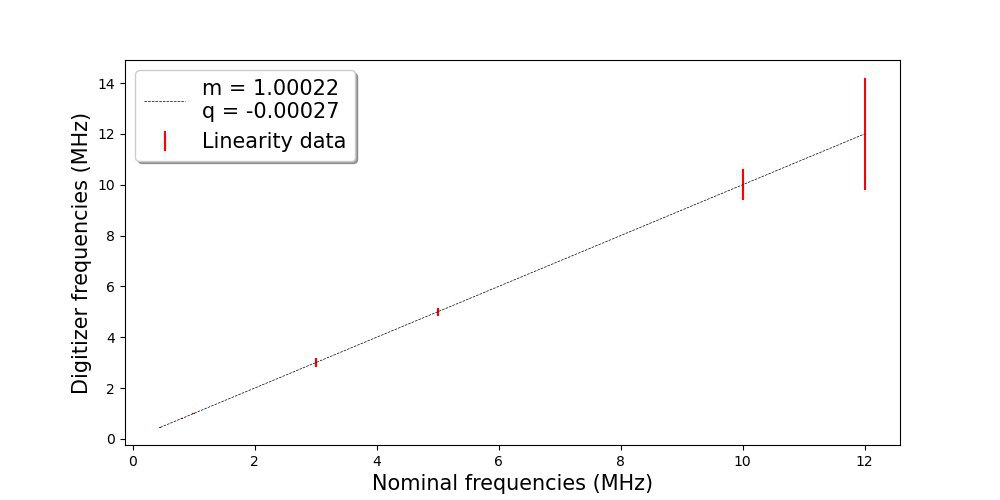
\includegraphics[width=.75\textwidth]{linearity_10}
	\caption{The data collected are reported in red and the fit function in a black dashed line. The errors are multiplied by a factor $10$ to highlight the small errors on the lower frequencies data.}
	\label{fig:digitizer_linearity}
\end{figure}
The data and the fit results are reported in Table \ref{tab:linearity_data} and first of all it is possible to see that the intercept of the fitting function is compatible with zero even if it is of no importance since exponential functions have been used the muon lifetime; in addition our data suggest a non-linearity smaller than $0.05\%$ and so it is possible to conclude that the non-linearity will be not taken into account in the later part of the experiment.
\begin{table}[!htp]
	\centering
	\begin{tabular}{rcc}
		\toprule
		\multicolumn{3}{c}{Fit results} \\
		\midrule
		Slope ($m$) &\multicolumn{2}{c}{$1.00022$} \\
		Intercept ($q$) &\multicolumn{2}{c}{$-0.00027$} \\
		Non-linearity ($\%$) &\multicolumn{2}{c}{$0.022$} \\
		\midrule
		\multicolumn{3}{c}{Data}\\
		\midrule
		Nominal Frequencies $\left[ \si{\mega\hertz}\right]$ & Measured Frequencies $\left[ \si{\mega\hertz}\right]$ & $\sigma \ \left[ \si{\mega\hertz}\right]$ \\
		\midrule
		$0.4500$ & $0.4500$ & $0.0004$ \\
		$0.5000$ & $0.5000$ & $0.0003$ \\
		$0.7000$ & $0.7000$ & $0.0008$ \\
		$0.8000$ & $0.8000$ & $0.0013$ \\
		$0.9900$ & $0.9901$ & $0.0020$ \\
		$1.0000$ & $1.0000$ & $0.0010$ \\
		$3.0000$ & $3.0001$ & $0.0169$ \\
		$5.0000$ & $5.0002$ & $0.0167$ \\
		$10.0000$ & $10.0004$ & $0.0607$ \\
		$12.0000$ & $12.0038$ & $0.2217$ \\
		\bottomrule
	\end{tabular}
	\caption{Fit results and recorded data.}
	\label{tab:linearity_data}
\end{table}

\section{Scintillators characterization}
The ideal detector should have various properties, in particular:
\begin{itemize}
	\item Perfect conversion of the kinetic energy of charged particles into light which must be detected with efficiency equal to $100\,\%$.
	\item Uniform light yield for each detector portion.
\end{itemize}
A further complication is given by the fact that the laboratory location is affected by a not-negligible natural background radiation which is mainly composed by photons.

As explained in Subsection~\ref{Mu-Sci}, plastic (organic) scintillators are preferred in timing measurements but, equally as any real detector, there are non-ideal behaviors that have to be recognized and taken into consideration before the subsequent muons lifetime measurements.

\subsection{Single-detector counting rates}
Background photons usually belong to energy ranges lower than the mean $\mu$-energy (at the ground) of about $\SI{4}{\giga\electronvolt}$, thus the employment of a discriminator module is a reasonable way to suppress them (the instruments configuration is shown in Figure \ref{fig:single-rate}).
\begin{figure}[!h]
	\centering
	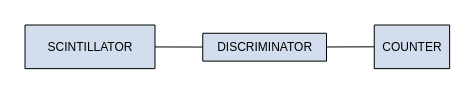
\includegraphics[width=.8\linewidth]{characterization/rate}
	\caption{Single-detector counting rates configuration.}
	\label{fig:single-rate}
\end{figure}

As a first step towards excluding $\gamma$-background, a study of both discriminator threshold and photo-multiplier bias voltages is carried out by taking into account one single detector at a time.\\

At fixed bias voltage, the expected behavior is the following: the higher threshold tension is, the lower counting rate is, until a \emph{plateau} is reached, when (ideally) all signals generated by background photons have been rejected and only muons are detected.\\
\begin{figure}[!htp]
	\centering
	\begin{subfigure}{.5\linewidth}
		\centering
		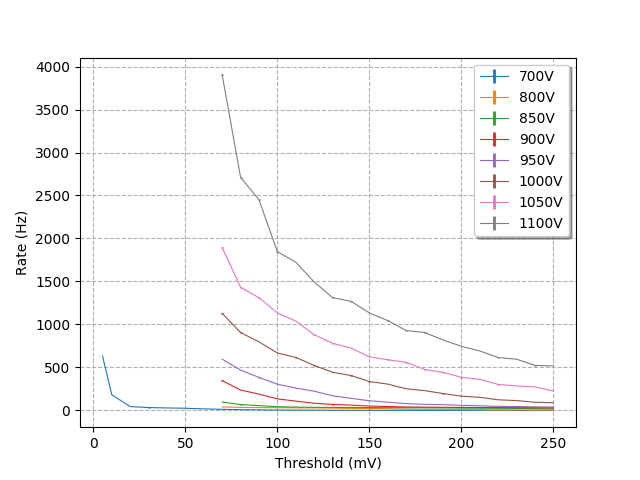
\includegraphics[width=\linewidth]{characterization/rate_threshold_caronte}
		\caption{\emph{Caronte}.} 
		\label{subfig:rt_caronte}
	\end{subfigure}\hfill
	\begin{subfigure}{.5\linewidth}
		\centering
		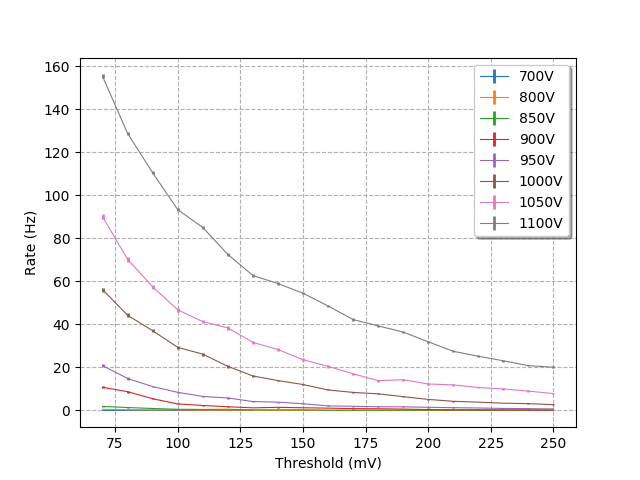
\includegraphics[width=\linewidth]{characterization/rate_threshold_cerbero}
		\caption{\emph{Cerbero}.} 
		\label{subfig:rt_cerbero}
	\end{subfigure}\hfill
	\begin{subfigure}{\linewidth}
		\centering
		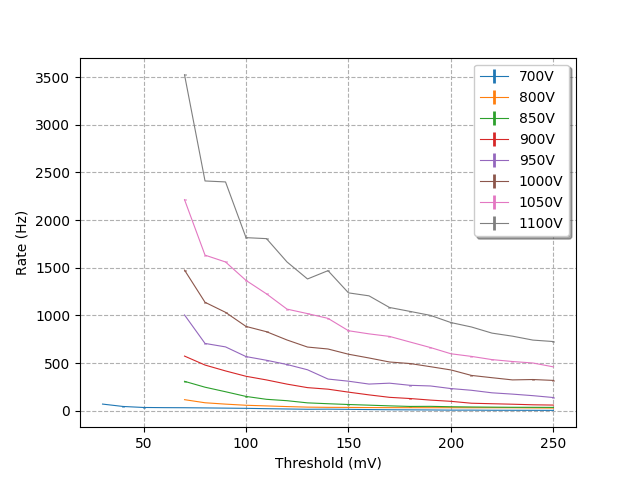
\includegraphics[width=.5\linewidth]{characterization/rate_threshold_minosse}
		\caption{\emph{Minosse}.} 
		\label{subfig:rt_minosse}
	\end{subfigure}
	\caption{Rate as a function of discriminator threshold tension, at fixed bias voltages. Errors on rates are calculated as $\sqrt{N}/t$, according to \emph{Poisson} probability distribution.} 
	\label{fig:rt}
\end{figure}

Figure \ref{fig:rt} highlights a more complicated trend, which is far from clarifying a suitable combination of threshold and bias voltages. Of course the most significant analysis will be performed concerning the detection efficiency (see Subsection \ref{sub:detection_eff}), but some aspects are worth considering, in fact it is important to note that the threshold can not be increased as desired since, after a certain value, in addition to photons, muons are rejected too. This behavior is clear if taking into consideration the obtained counting rates lower than the $\approx\SI{40}{\hertz}$ expected muons one.

By comparing \emph{Caronte} (Figure \ref{subfig:rt_caronte}) and \emph{Minosse} (Figure \ref{subfig:rt_minosse}) with \emph{Cerbero} (Figure \ref{subfig:rt_cerbero}), we can predict that the latter is definitely less efficient than the former detectors. Moreover, when working at low bias voltages (e.g. $\SI{700}{\volt}$), even the lowest considered thresholds are sufficient to cut most of the signal and we are legitimated to suspect that higher bias tensions should be preferred.\\
\begin{figure}[!htp]
	\centering
	\begin{subfigure}{.5\linewidth}
		\centering
		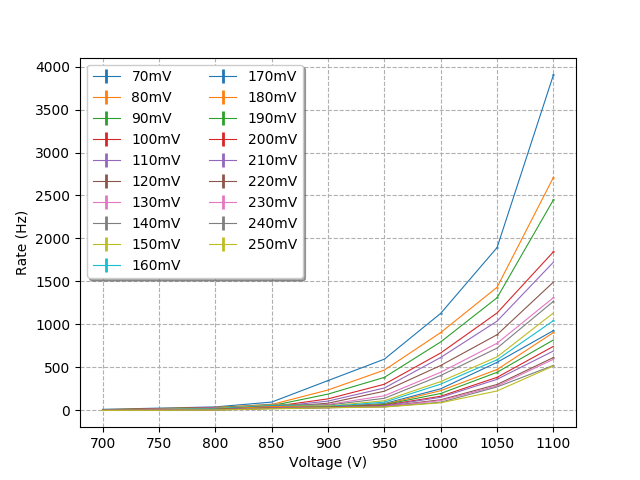
\includegraphics[width=\linewidth]{characterization/rate_bias_caronte}
		\caption{\emph{Caronte}.} 
		\label{subfig:rb_caronte}
	\end{subfigure}\hfill
	\begin{subfigure}{.5\linewidth}
		\centering
		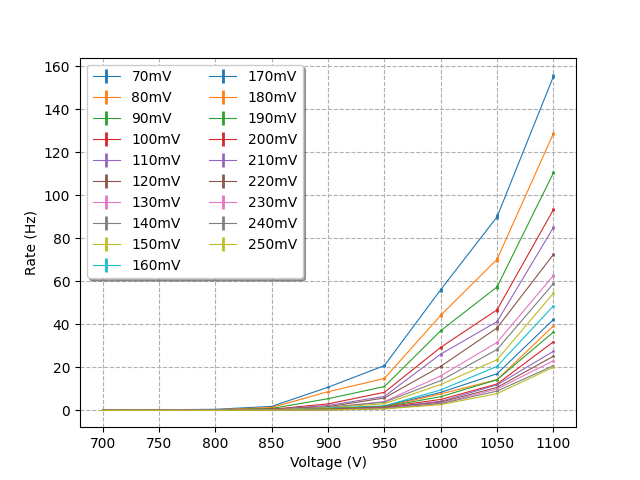
\includegraphics[width=\linewidth]{characterization/rate_bias_cerbero}
		\caption{\emph{Cerbero}.} 
		\label{subfig:rb_cerbero}
	\end{subfigure}\hfill
	\begin{subfigure}{.5\linewidth}
		\centering
		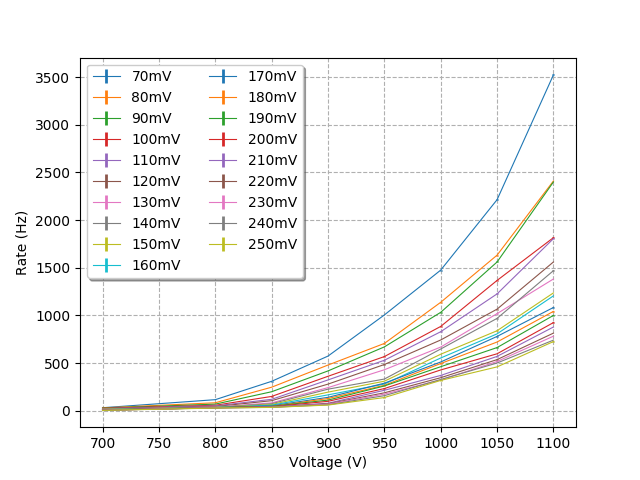
\includegraphics[width=\linewidth]{characterization/rate_bias_minosse}
		\caption{\emph{Minosse}.} 
		\label{subfig:rb_minosse}
	\end{subfigure}
	\caption{Rate as a function of bias voltage, at fixed discriminator thresholds. Errors on rates are calculated as $\sqrt{N}/t$, according to \emph{Poisson} probability distribution.} 
	\label{fig:rb}
\end{figure}

\begin{figure}[!htp]
	\centering
	\begin{subfigure}{\linewidth}
		\centering
		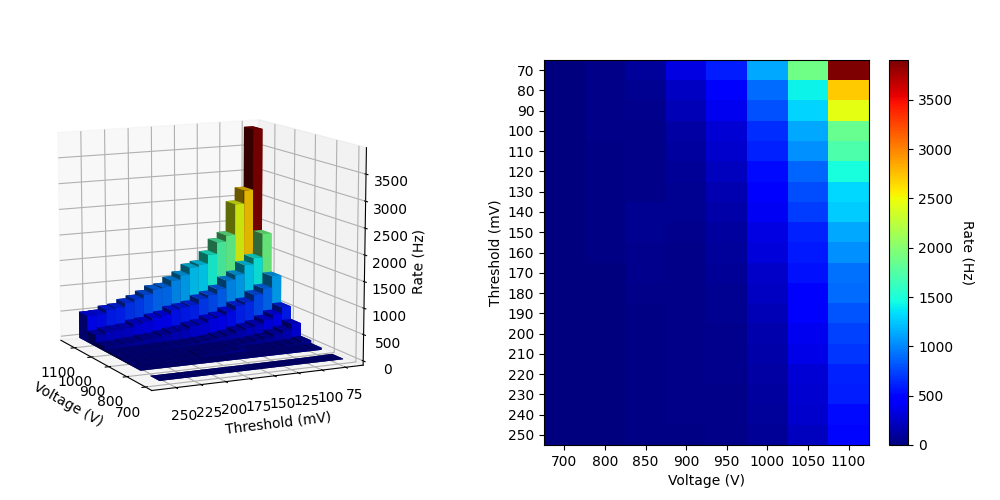
\includegraphics[width=.9\linewidth]{characterization/3d_caronte}
		\caption{\emph{Caronte}.} 
		\label{subfig:3d_caronte}
	\end{subfigure}\hfill
	\begin{subfigure}{\linewidth}
		\centering
		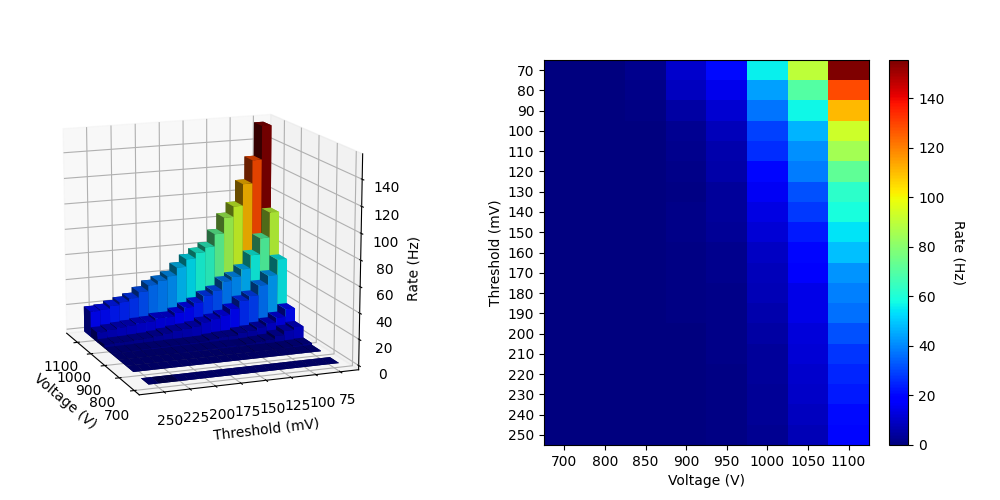
\includegraphics[width=.9\linewidth]{characterization/3d_cerbero}
		\caption{\emph{Cerbero}.} 
		\label{subfig:3d_cerbero}
	\end{subfigure}\hfill
	\begin{subfigure}{\linewidth}
		\centering
		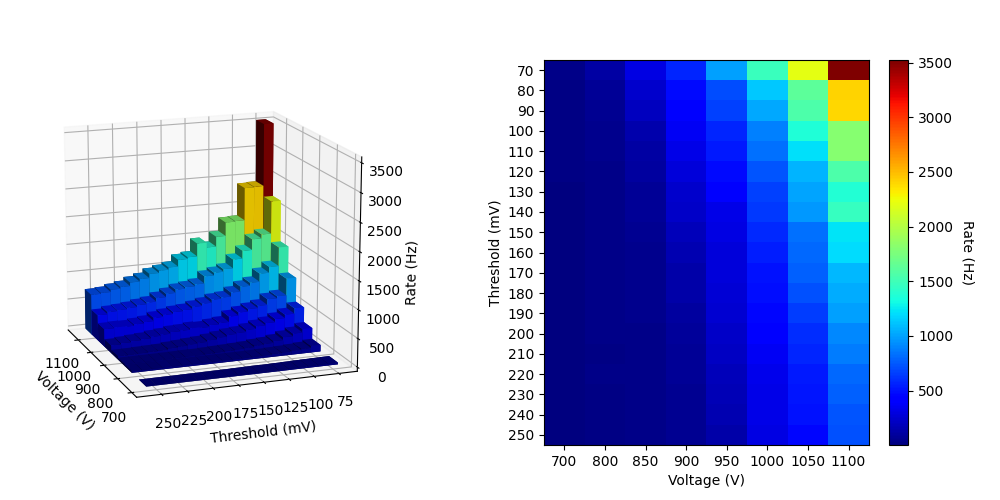
\includegraphics[width=.9\linewidth]{characterization/3d_minosse}
		\caption{\emph{Minosse}.} 
		\label{subfig:3d_minosse}
	\end{subfigure}
	\caption{Rate as a function of threshold and bias voltages. 3D plot (on the left) and heat-map (on the right).} 
	\label{fig:3d}
\end{figure}
%\begin{figure}
%	\ContinuedFloat
%	\begin{subfigure}{\linewidth}
%		\centering
%		\includegraphics[width=.7\linewidth]{characterization/3d_mino
%		e}
%		\caption{\emph{Minosse}.} 
%		\label{subfig:3d_minossex}
%	\end{subfigure}
%\end{figure}

Instead, a study of single-detector counting rates at fixed discriminator threshold is represented in Figure \ref{fig:rb}. Data shown in Figure \ref{fig:rt} and \ref{fig:rb} are then combined in Figure \ref{fig:3d}, allowing an overall sight.\\

As above-mentioned, the interesting feature that has to be studied is the efficiency, however the single-detector counting rates are useful, meaning that they can give a first rough idea of what is the region of voltages from which is worth beginning the efficiencies analysis. In fact, by observing the zoomed-in Figure \ref{fig:zoomed} plots, we can identify a flattening behavior in the neighborhood of $\sim \SI{40}{\hertz}$ for \emph{Caronte} and  \emph{Minosse}, whilst  \emph{Cerbero} does not exhibit a similar trend, justifying the suspected low detection efficiency.

\begin{figure}[!htp]
	\centering
	\begin{subfigure}{.5\linewidth}
		\centering
		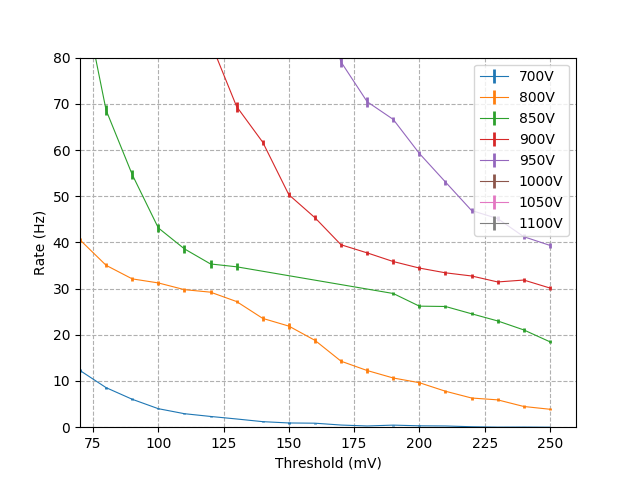
\includegraphics[width=\linewidth]{characterization/rate_threshold_caronte_zoomed}
		\caption{\emph{Caronte}.} 
		\label{subfig:zoomed_caronte}
	\end{subfigure}\hfill
	\begin{subfigure}{.5\linewidth}
		\centering
		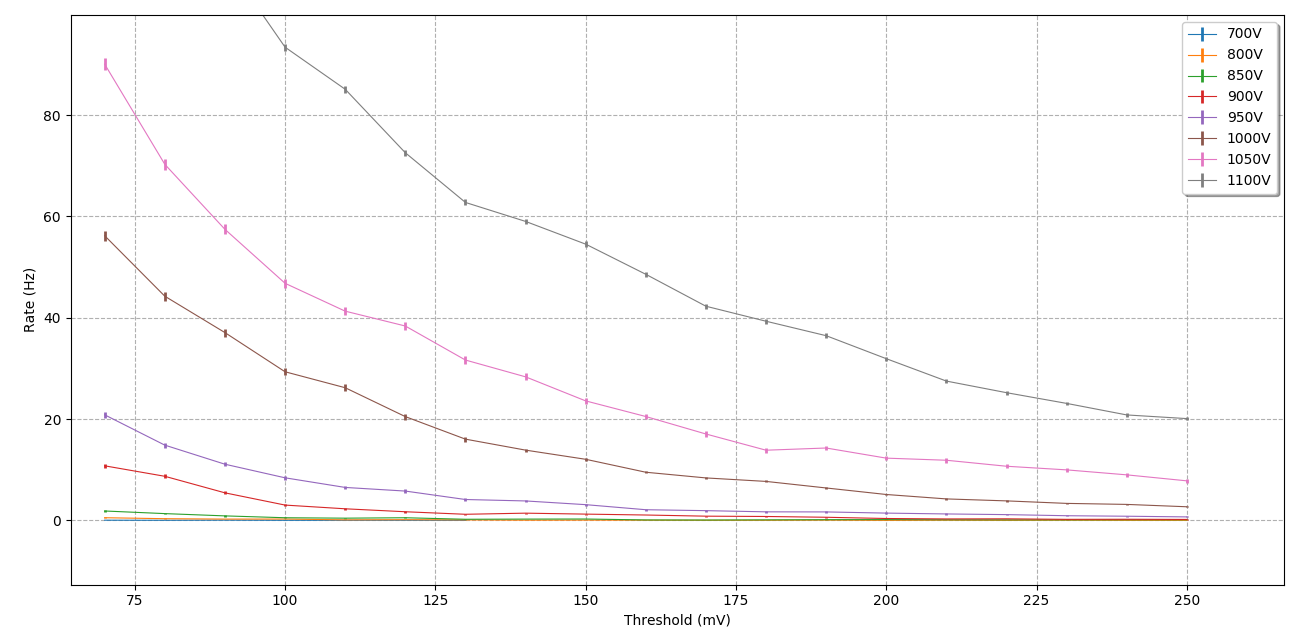
\includegraphics[width=\linewidth]{characterization/rate_threshold_cerbero_zoomed}
		\caption{\emph{Cerbero}.} 
		\label{subfig:zoomed_cerbero}
	\end{subfigure}\hfill
	\begin{subfigure}{\linewidth}
		\centering
		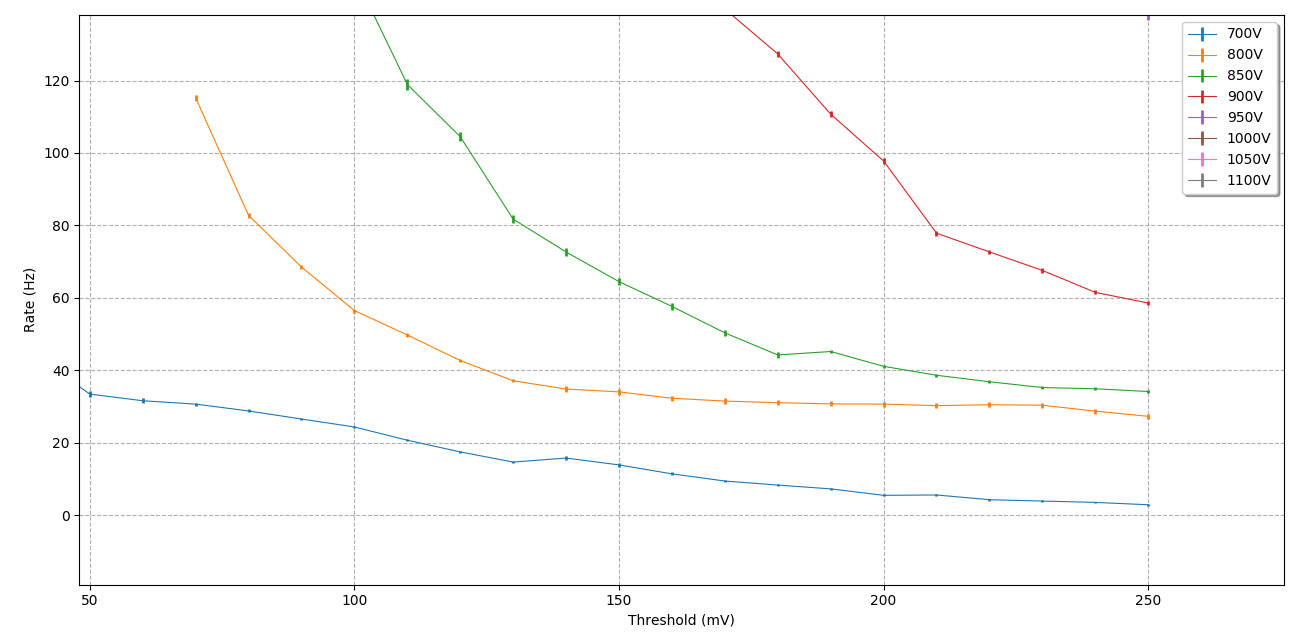
\includegraphics[width=.5\linewidth]{characterization/rate_threshold_minosse_zoomed}
		\caption{\emph{Minosse}.} 
		\label{subfig:zoomed_minosse}
	\end{subfigure}
	\caption{Rate as a function of discriminator threshold tension, at fixed bias voltages. Magnification on plateau areas of Figure \ref{fig:rb}.} 
	\label{fig:zoomed}
\end{figure}



\subsection{Detection efficiency} \label{sub:detection_eff}

Of course, a condition where detectors work with the highest efficiencies is fundamental and thus a setup that is suitable for efficiency estimation has to be prepared.
\begin{figure}[!h]
	\centering
	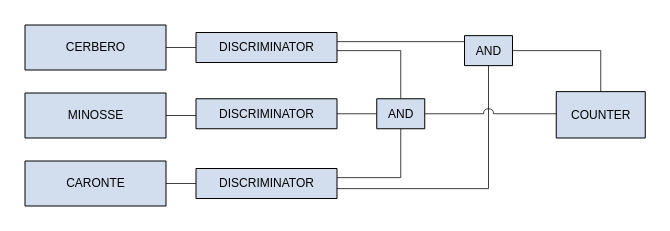
\includegraphics[width=.8\linewidth]{characterization/efficiency}
	\caption{Efficiency studies setup.}
	\label{fig:eff-setup}
\end{figure}
With an aligned geometry (where the three $80\times 30$ cm scintillators are one above the other) the detection efficiency of the middle detector can be easily calculated as
\begin{equation}
\varepsilon = \frac{N_{triple}}{N_{double}}
\end{equation}
where $N_{double}$ is the number of coincidences between the upper scintillator and the lower one, instead $N_{triple}$ is given by the coincidence of all detector signals. Figure \ref{fig:eff-setup} is a pictorial diagram of the instrumentation setup. The \texttt{AND} ports are realized by means of a programmable logic unit.\\
\begin{figure}[!bp]
	\centering
	\begin{subfigure}{.5\linewidth}
		\centering
		\includegraphics[width=\linewidth]{characterization/eff_caronte}
		\caption{\emph{Caronte}.} 
		\label{subfig:eff_caronte}
	\end{subfigure}\hfill
	\begin{subfigure}{.5\linewidth}
		\centering
		\includegraphics[width=\linewidth]{characterization/eff_cerbero}
		\caption{\emph{Cerbero}.} 
		\label{subfig:eff_cerbero}
	\end{subfigure}\hfill
\end{figure}
\begin{figure}[!ht]
	\centering
	\ContinuedFloat
	\begin{subfigure}{.5\linewidth}
	\centering
	\includegraphics[width=\linewidth]{characterization/eff_minosse}
	\caption{\emph{Minosse}.} 
	\label{subfig:eff_minosse}
	\end{subfigure}
	\caption{Detection efficiencies.} 
	\label{fig:eff}
\end{figure}

Figure \ref{fig:zoomed} highlights which configurations of bias and threshold voltages are advisable in order to work mainly with muons and be left with a little-to-no $\gamma$-background, therefore the scintillators efficiencies represented in Figure \ref{fig:eff}  (data are contained in Appendix \ref{app:eff}) give a clear information of the bias-threshold setup that has to be avoided so as to guarantee the largest light yield.\\

Concerning the efficiency estimation from a statistical perspective, and considering that
\begin{equation}\label{eq:binomial}
N_{triple}=N_{double}\cdot\varepsilon
\end{equation}
the number of triple counts is nothing but the result of \emph{Bernoulli} trial where $N_{double}$ is the total number of trials and $\varepsilon$ is the probability of success, i.e. the particle is effectively detected by the middle detector. Therefore, the uncertainty on $N_{triple}$ is due to the binomial probability distribution:
\begin{equation}
\sigma_{triple}=\sqrt{N_{double}\cdot\varepsilon\left(1-\varepsilon\right)}
\end{equation}
and, according to propagation of errors formula, we end up with
\begin{equation}\label{eq:eff_err}
\sigma_{\varepsilon}=\sqrt{\frac{\varepsilon\left(1-\varepsilon\right)}{N_{double}}}=\displaystyle\frac{1}{N_{double}}\sqrt{N_{triple}\left(1-\frac{N_{triple}}{N_{double}}\right)}
\end{equation}
\eqref{eq:eff_err} is the expression which error bars on efficiency have been conveniently calculated with.\\

Finally, the chosen configuration is summed up in Table \ref{tab:bt-setup}.
\begin{table}[!hb]
	\centering
	\begin{tabular}{r|ccc}
		\toprule
		Detector&Bias Voltage (V)&Threshold tension (mV)&Efficiency $\varepsilon$\\
		\midrule
		\emph{Caronte} & $900$ & $170$ & $0.9937\pm 0.0013$\\
		\emph{Cerbero} & $1000$ & $40$ & $0.9938\pm 0.0013$\\
		\emph{Minosse} & $850$ & $180$ & $0.9948\pm 0.0011$\\
		\bottomrule
	\end{tabular}
	\caption{Bias-threshold setups that have been chosen for physics measurements.}
	\label{tab:bt-setup}
\end{table}


\subsection{Uniformity of light yield}

\label{sec:uniformity}

In the previous section an overall efficiency has been calculated for each scintillator, but we are interested in understanding if the detector light yield keeps itself unvaried through different portions, thus the conclusive analyses in terms of the detectors characterization are the uniformity studies.\\

\begin{figure}[!hbtp]
	\centering
	\begin{subfigure}{.3\linewidth}
		\centering
		\includegraphics[width=\linewidth]{characterization/uniformity1}
		\caption{First layout.} 
		\label{subfig:uniformity1}
	\end{subfigure}\hfill
	\begin{subfigure}{.3\linewidth}
		\centering
		\includegraphics[width=\linewidth]{characterization/uniformity2}
		\caption{Second layout.} 
		\label{subfig:uniformity2}
	\end{subfigure}\hfill
	\begin{subfigure}{.3\linewidth}
		\centering
		\includegraphics[width=\linewidth]{characterization/uniformity3}
		\caption{Third layout.} 
		\label{subfig:uniformity3}
	\end{subfigure}
	\caption{Detectors setup during uniformity studies. From below: \emph{Caronte}, \emph{Minosse}, \emph{Cerbero}.}
	\label{fig:uniformity}
\end{figure}

The instrumentation setup is unchanged with respect to Figure \ref{fig:eff-setup}, however the geometrical layout is no longer aligned, but organized for a specific area study, as Figure \ref{fig:uniformity} illustrates.\\

Before presenting the results of the analyses we call attention to the fact that efficiency can not be calculated as the ratio of $N_{triple}$ to  $N_{double}$ anymore, as a consequence of a geometrical effect previously explained in Section \ref{sec:uniformity_studies}. Therefore, the correct formula is \eqref{eq:eff_correct} where $\varepsilon_{g}$ comes from the Monte Carlo simulations, whose results are collected in Table \ref{tab:err-effg}.\\

The errors take into account both the statistical nature due to the binomial probability distribution of $N_{triple}$ and the systematical uncertainty estimated on $\varepsilon_{g}$ (see Table \ref{tab:err-effg}), hence we have $\varepsilon\pm \sigma_{\varepsilon}^{stat} \pm \sigma_{\varepsilon}^{sys}$ where
\begin{equation}
\sigma_{\varepsilon}^{stat}=\displaystyle\frac{1}{\varepsilon_{g}\cdot N_{double}}\sqrt{N_{triple}\left(1-\frac{N_{triple}}{\varepsilon_{g}\cdot N_{double}}\right)}
\end{equation}
and
\begin{equation}
\sigma_{\varepsilon}^{sys}=\frac{N_{triple}\cdot\sigma_{\varepsilon_{g}}}{\varepsilon_{g}^2\cdot N_{double}}
\end{equation}

\begin{table}[!bht]
	\centering
	\begin{tabular}{r|ccc}
		\toprule
		&$N_{triple}$&$N_{double}$&$\varepsilon\pm\sigma_{\varepsilon}^{stat}\pm\sigma_{\varepsilon}^{sys}$\\
		\midrule
		Layout 1 &$4975$ & $5406$ & $0.979\pm 0.002 \pm 0.005$\\
		Layout 2 &$5332$ & $5746$	& $0.9893\pm 0.0014 \pm 0.005$\\
		Layout 3 &$3473$ & $3947$ & $0.987\pm 0.002 \pm 0.010$\\
		\bottomrule	
	\end{tabular}
	\caption{Layouts efficiencies, \emph{Caronte}.}\label{tab:unif_caronte}
\end{table}
\begin{table}[!hbt]
	\centering
	\begin{tabular}{r|ccc}
		\toprule
		&$N_{triple}$&$N_{double}$&$\varepsilon\pm\sigma_{\varepsilon}^{stat}\pm\sigma_{\varepsilon}^{sys}$\\
		\midrule
		Layout 1 &$4320$ & $4803$ & $0.9928\pm 0.0013\pm 0.006$\\
		Layout 2 &$4991$ & $5606$	& $0.9848\pm 0.0017\pm 0.006$\\
		Layout 3 &$3455$ & $4081$ & $0.9960\pm 0.0011\pm 0.009$\\
		\bottomrule	
	\end{tabular}
	\caption{Layouts efficiencies, \emph{Cerbero}.}\label{tab:unif_cerbero}
\end{table}
\begin{table}[!tb]
	\centering
	\begin{tabular}{r|ccc}
		\toprule
		&$N_{triple}$&$N_{double}$&$\varepsilon\pm\sigma_{\varepsilon}^{stat}\pm\sigma_{\varepsilon}^{sys}$\\
		\midrule
		Layout 1 &$4916$ & $5279$ & $0.9907\pm 0.0014\pm 0.005$\\
		Layout 2 &$5428$ & $5837$	& $0.9914\pm 0.0013\pm0.005$\\
		Layout 3 &$3768$ & $4356$ & $0.970\pm 0.003\pm 0.010$\\
		\bottomrule	
	\end{tabular}
	\caption{Layouts efficiencies, \emph{Minosse}.}\label{tab:unif_minosse}
\end{table}


For each scintillator, the resulting efficiencies (Table \ref{tab:unif_caronte}, \ref{tab:unif_cerbero} and \ref{tab:unif_minosse}) reveal normalized deviations that span in the range $0.1$-$1.8$ (see Table \ref{tab:norm_dev}). \emph{Cerbero} results are compatible with the hypothesis of a uniform detector and are in agreement with the efficiency estimated in the aligned setup.  
Notwithstanding the \emph{Caronte} and \emph{Minosse} results could suggest the evidence of some non-uniformity, we can see that efficiencies are systematically underestimated with respect to the overall ones showed in Table \ref{tab:bt-setup}, therefore it is clear that the geometrical weight estimated by means of the Monte Carlo procedure is not enough to cure the inconsistencies due to systematic errors encountered with these detectors.

\begin{table}[!hbt]
	\centering
	\begin{tabular}{r|ccc}
		\toprule
		Detector&$t_{12}$&$t_{13}$&$t_{23}$\\
		\midrule
		Caronte &$1.4$ & $1.4$ & $0.2$\\
		Cerbero &$0.9$ & $0.3$ & $1.0$\\
		Minosse &$0.1$ & $1.8$ & $1.8$\\
		\bottomrule	
	\end{tabular}
	\caption{Normalized deviations calculated as $t_{ij}=\left|\varepsilon_{i}-\varepsilon_{j}\right|/\sqrt{\sigma_{\varepsilon_{i}}^2+\sigma_{\varepsilon_{j}}^2}$ where $i,j$ are referred to layouts.}\label{tab:norm_dev}
\end{table}

The evidence of an additional systematic error\footnote{Since the distance between scintillators with \emph{Caronte} in the middle position is the same of \emph{Minosse} as middle detector, we could suspect that a mistake has been made while measuring the distances.} we have not identified led us to make one extra uniformity measurements session, by means of a new littler $27.5\times \SI{8.3}{cm}$ plastic scintillator, whose bias voltage and discrimination threshold tension have been set to $\SI{1550}{V}$ (according to the manufacturer recommendations) and $\SI{40}{mV}$, respectively. The acquisition time is $20$ minutes, in order to collect sufficient counts and reduce the statistical uncertainty.
\begin{figure}[!htb]
	\centering
	\includegraphics[width=.29\linewidth]{characterization/Paletta}
	\caption{Detectors setup during fine uniformity studies. From below: \emph{Caronte}, \emph{Minosse}, ``new'' scintillator.} \label{fig:fine_unif}
\end{figure}

This part of the analysis has been carried out only referring to \emph{Minosse} (the geometrical setup is shown in Figure \ref{fig:fine_unif}). Table \ref{tab:fine_eff} shows the results of the study, whose graphical representation is given in Figure \ref{fig:fine_eff}.\\

\begin{table}
	\centering
	\begin{tabular}{r|ccc}
		\toprule
		&$N_{triple}$&$N_{double}$&Efficiency $\varepsilon$\\
		\midrule
		Area 1 & $1312$	& $1314$ &	$0.9985\pm	0.0011$\\
		Area 2 & $1379$	& $1382$ &	$0.9978\pm	0.0013$\\
		Area 3 & $1184$	& $1188$ &	$0.9966\pm	0.0017$\\
		Area 4 & $1519$	& $1521$ &	$0.9987\pm	0.0009$\\
		Area 5 & $1584$	& $1589$ &	$0.9969\pm	0.0014$\\
		Area 6 & $2352$	& $2352$ &	$1.0000\pm	0.0000$\\
		Area 7 & $2334$	& $2336$ &	$0.9991\pm	0.0006$\\
		Area 8 & $1917$	& $1920$ &	$0.9984\pm	0.0009$\\
		Area 9 & $1655$	& $1660$ &	$0.9970\pm	0.0014$\\
		\bottomrule
	\end{tabular}
    \caption{\emph{Minosse} efficiencies during fine uniformity studies. The uncertainty on $\varepsilon$ has been computed according to \eqref{eq:eff_err}.} \label{tab:fine_eff}
\end{table}

Except for too small errors on the efficiencies which may cause possible discrepancies, we do not observe problematic behaviors in any portion of the detector.

\begin{figure}[!bht]
	\centering
	\includegraphics[width=.8\linewidth]{characterization/fine_uniformity_minosse}
	\caption{\emph{Minosse} efficiencies during fine uniformity studies.} \label{fig:fine_eff}
\end{figure}


\chapter{Lifetime measurement}
\section{DAQ Trigger}
In this chapter we describe how to perform muon lifetime measurments. The electronic chain used for the signal processing is shown in Figure \ref{fig::trigger}.
The scintillators are supplied by the bias voltages reported in Table \ref{tab:bt-setup} and the anodic output signals enter the discriminator to reject background events (thresholds are set according to Table \ref{tab:bt-setup} too).
Before entering the trigger system, the discriminator outputs are multiplied by means of a Fan-In/Fan-Out unit, hence the signals from the upper and the lower scintillators are sent to CH0 and CH1 of the digitizer. The rest of the electronic chain is set in order to perform start and stop topologies for the muon decay triggering. 

\begin{figure}[!h]
	\centering
	\includegraphics[scale=0.5]{lifetime/trigger}
	\caption{Electronic chain and trigger system used for muon lifetime measurments.}
	\label{fig::trigger}
\end{figure}

\subsection{Trigger system}
To acquire only muon decay events it is necessary to build a trigger system as the one reported in Figure \ref{fig::trigger}, which provides an \emph{external trigger} signal for the digitizer. Therefore the digitizer acquires \emph{Cerbero} and \emph{Caronte} waveforms only for those events which satisfy the trigger requirements.
The trigger signal consists in the logic coincidence (\texttt{AND} operation) between a START and a STOP, marking respectively the decay of the muon in the middle scintillator and the release of energy by the charged decay product in one of the external detectors. Figure \ref{fig::scinti_decay} shows a scheme for a possible muon decay event which gives a START event and its corresponding STOP event in the external scintillators.

\subsection{Start}
The START signal corresponds to the capture of the muon in the middle scintillator. This event involves the release of energy in the upper (1) and in the middle detector (2) but not in the lower one (3). Therefore, the START signal is produced by the $1 \wedge 2 \wedge \overline{3}$ topology.\\

The pulses coming from the scintillators are sent into the discriminator module and its output is multiplied by a Fan-In/Fan-Out. The three signals are sent to a programmable logic unit to perform logic \texttt{AND} operation. 
Using the dual timer the START is widened up to $5 \tau_{\mu} \simeq \SI{11}{\micro s}$, which is the period of time in which we expect the most of the selected muons to decay.  %Hence the apparatus is sensible to time measures in the range $[0, 11] \si{\micro s}$.\\
Note that since all START events satisfies also the STOP topology $1 \wedge \overline{3}$, the START signal is delayed of $\sim \SI{50}{\nano s}$ by means of a delay unit and LEMO cables in order to prevent fake trigger events caused by auto-coincidences.

\begin{figure}[!h]
	\centering
	\includegraphics[scale=0.44]{lifetime/scinti_decay}
	\caption{Scheme of a possible muon decay event. The incident muon stops in the middle scintillator (START with $1 \wedge 2 \wedge \overline{3}$ topology). The muon decays releasing energy in the upper or in the lower scintillator (STOP with $1 \land \overline 3$ or $\overline 1 \land 3$ respectively).}
	\label{fig::scinti_decay}
\end{figure}

Actually, the START topology does not guarantee uniquely that a muon decay event has happened. In fact there is also the possibility for a muon to cross 1 and 2 without crossing 3 because of the geometric acceptance (see Figure \ref{start_false}).

\begin{figure}[!thp]
	\centering
	\begin{subfigure}{.3\linewidth}
		\centering
		\includegraphics[width=\linewidth]{lifetime/start_true}
		\caption{True START: $\mu$ crosses 1 and 2 stopping in it.}
		\label{start_true}
	\end{subfigure}
	\begin{subfigure}{.3\linewidth}
		\centering
		\includegraphics[width=\linewidth]{lifetime/start_false}
		\caption{False START: $\mu$ crosses 1 and 2 without stopping in it.}\label{start_false}
	\end{subfigure}
	\caption{Schemes of true and false START events.}
	\label{}
\end{figure}


\subsection{Stop} 
The STOP signal corresponds to the loss of energy of the charged lepton produced in the decay in one of the outer scintillators. To produce the STOP signal a programmable logic unit is used to perform an \texttt{AND} operation between the signals from the external detectors. In this way it is possible to select only event topologies corresponding to a charged lepton which crosses the upper scintillator and not the lower one ($1 \wedge \overline 3$) or vice versa ($\overline 1 \wedge 3$). The output of these logic operations are sent into a coincidence unit performing an \texttt{OR} operation between the two STOPs, obtaining the overall STOP topology $ (1 \land \overline 3) \lor (\overline 1 \land 3) $.
Finally, a logical \texttt{AND} is performed between the overall STOP and the widened and delayed START signals.\\
Note that false STOP events could happen due to the detectors geometric acceptance. Nevertheless these STOP events are less probable as they are suppressed by the $\cos^{2} \theta$ angular distribution. Figure \ref{false_stop_events} shows some examples of possible false STOP events.


\begin{figure}[!thp]
	\centering
	\begin{subfigure}{.26\linewidth}
		\centering
		\includegraphics[width=\linewidth]{lifetime/falso_stop}
		\caption{False $ (1 \land \overline 3)$ STOP.}
		\label{false_stop}
	\end{subfigure}
	\begin{subfigure}{.26\linewidth}
		\centering
		\includegraphics[width=\linewidth]{lifetime/falso_stop_2}
		\caption{False $ (\overline 1 \land  3)$ STOP.}
		\label{false_stop_2}
	\end{subfigure}
	\begin{subfigure}{.26\linewidth}
		\centering
		\includegraphics[width=\linewidth]{lifetime/falso_stop_3}
		\caption{False $ (1 \land \overline 3) \lor (\overline 1 \land 3) $ STOP.}
		\label{false_stop_3}
	\end{subfigure}
	\caption{Schemes of possible false STOP events.}\label{false_stop_events}
\end{figure}

\subsection{Further observations} \label{obs}
Since the trigger system has been built using many electronic modules and different cables, it is of primary importance to keep under control all the delays introduced during the configuration of the electronic chain. For this reason, during the construction of the trigger system, the input-output delays of each module have been taken into account and LEMO cables of suitable length have been used in order to have signals which reach the programmable logic unit gates all with the same delay.\\
%In Figure \ref{fig:osc_coinc} is shown the oscilloscope visualization of the START and STOP signals which enter the final Coincidence Unit in \texttt{AND} mode and whose coincidence gives the trigger signal. Note that in Fig. \ref{subfig::strat_stop_delay} the START signal has been conveniently delayed respect to the STOP signal in order to prevent fake coincidences (i.e. START autocoincidences). The STOP signal outgoing the logic $\texttt{OR}$ gate exhibits a double square pulse which is due to signal rebouincing and can be prevented widening the gate width of the Coincidence Unit in $\texttt{OR}$ mode up to $\sim \SI{100}{ns}$.  In Figure \ref{subfig::eccoilmu} is shown the evidence of a muon decay event given by the coincidence of the START and STOP signals. Note how the use of the Dual Timer to extend the start signal up to $\SI{11}{\micro s}$ is necessary to detect muon decay events.\\
%\begin{figure}[!htp]
%	\centering
%	\begin{subfigure}{.45\linewidth}
%		\centering
%		\includegraphics[width=\linewidth]{lifetime/TEK00002}
%		\caption{The START signal is delayed to prevent fake coincidences. }
%		\label{subfig::strat_stop_delay}
%	\end{subfigure}\hfill
%	\begin{subfigure}{.45\linewidth}
%		\centering
%		\includegraphics[width=\linewidth]{lifetime/TEK00003}
%		\caption{Evidence of a muon decay given by an $\texttt{AND}$ coincidence between the START and STOP signal.}
%		\label{subfig::eccoilmu}
%	\end{subfigure}
%	\caption{Oscilloscope visualization. The white line represents the START signal while purple line represents the STOP signal outgoing the Coincidence Unit in \texttt{OR} mode.}
%	\label{fig:osc_coinc}
%\end{figure}

Figure \ref{fig:fin} shows the oscilloscope visualization of the anodic output of \emph{Cerbero}, its discriminator output and the programmable logic unit $1 \land \overline{3}$ output signal. In Subsection \ref{discriminator} \emph{Cerbero} discriminator width was set to $\SI{80}{\nano s}$ in order to prevent false double or triple counts due to the considerable noise fluctuations. In this case, since \emph{Cerbero} discriminator output is twice the \emph{Caronte} one, the effect is to get multiple STOPs given by the fake coincidences of different signals detected in \emph{Caronte} within the discriminator width of a single \emph{Cerbero} signal.
For this reason, \emph{Cerbero} discriminator width has been restricted up to $\SI{57.6}{\nano s}$.


\begin{figure}[!htp]
	\centering
	\begin{subfigure}{.45\linewidth}
		\centering
		\includegraphics[width=\linewidth]{lifetime/TEK00005}
		\caption{Logic coincidence $1 \land \overline 3$.}
	\end{subfigure}\hfill
	\begin{subfigure}{.45\linewidth}
		\centering
		\includegraphics[width=\linewidth]{lifetime/TEK00006}
		\caption{Fake logic coincidence $1 \land \overline 3$.}
	\end{subfigure}
	\caption{Oscilloscope visualization. The yellow line represents \emph{Cerbero} anodic output, the blue line is the discriminator output and the green line represents the programmable logic unit $1 \land \overline{3}$ output signal.}
	\label{fig:fin}
\end{figure}

\section{DAQ software}
\label{DAQ}
Events data acquisition is performed thanks to the CAEN Digitizer. In particular, pulses\footnote{The Digitizer requires standard NIM inputs, thus the two incoming signals are taken after the discrimination stage.} from the upper detector and the lower one are sent to Digitizer channels 0 and 1, respectively and they are actually acquired only when the external trigger green-lights it.\\

Digitizer saves events by using \texttt{.XML} format, which means \emph{eXstensible Markup Language}. The extend-ability of this language is given by the possibility to define personalized tags, extremely useful in order to organize data within a specific logic. Hence, after a prior analysis of the \texttt{XML} structure, a parser based on \texttt{BeautifulSoup4 Python} library has been developed (see Appendix \ref{app:xml_parser}): each triggered event is stored in a \texttt{ROOT TDirectory} and it consists of two waveforms (channels 0 and 1) saved as \texttt{TGraph}s. The \texttt{XML\_parser} output is given by a \texttt{TFile}. This first step is needed since lifetime measurements collect a lot of thousands of events and a well organized data structure is certainly a plus.\\

The interesting events are distinguished by two pulses: the first one is the passage of a $\mu^\pm$ through the upper scintillator, whilst the second one is caused by the emitted $e^\pm$ and it can be recorded both in the upper or the lower detector. For this reason a first skim that discards all the other types of events has been implemented (Figure \ref{fig:rej} gives two examples of rejected events).\\

The final stage of the DAQ software consists in the computing of the time shifts $\Delta t$ through the two waveforms: instead of fitting the pulses (in a partial range) by means of \emph{Fermi-Dirac}-like functions, a method based on the pulse derivative\footnote{The derivative of a square pulse is a Dirac-$\delta$.} (see Figure \ref{fig:derivative}) is performed due to the smaller computational cost and the distance between peaks is easily obtained.

\begin{figure}[!htp]
	\centering
	\begin{subfigure}{.5\linewidth}
		\centering
		\includegraphics[width=\linewidth]{lifetime/rejected1}
	\end{subfigure}\hfill
	\begin{subfigure}{.5\linewidth}
		\centering
		\includegraphics[width=\linewidth]{lifetime/rejected2}
	\end{subfigure}
	\caption{Examples of rejected events.}
	\label{fig:rej}
\end{figure}

\begin{figure}[!htp]
	\centering
	\begin{subfigure}{.5\linewidth}
		\centering
		\includegraphics[width=\linewidth]{lifetime/up_decay}
		\caption{Electron/positron emitted towards the\\ upper detector.}
	\end{subfigure}\hfill
	\begin{subfigure}{.5\linewidth}
		\centering
		\includegraphics[width=\linewidth]{lifetime/down_decay}
		\caption{Electron/positron emitted towards the\\ lower detector.}
	\end{subfigure}
	\caption{The upper plots represents the waveforms, while the lower plots are their derivatives. The time shift is calculated as the distance between the peaks minimums.} \label{fig:derivative}
\end{figure}

\section{Preliminary studies}
Offline data analyses have been made on the triggered signals: the Digitizer acquires \emph{Cerbero} and \emph{Caronte} waveforms and the DAQ software allows us to distinguish between STOPs in the upper or in the lower detector. A histogram is filled with different $\Delta t$s and what we expect is a negative exponential trend given by

\begin{equation} \label{exp}
N(\Delta t) = N_0\cdot e^{-\Delta t/\tau} + B
\end{equation}
where $\tau$ is the muon lifetime and $B$ is the uniform background due to random coincidences (see Appendix \ref{Background} for further details for the background estimation). 

\subsection{Preliminary lifetime measurements}
A first measurement campaign has been performed with the setup shown in Table \ref{tab:bt-setup}.
\begin{table}[!h]
	\centering
	\begin{tabular}{ccc||ccc}
		\toprule
		Up pulses & Down pulses & $N$ & Up pulses & Down pulses & $N$\\
		\midrule
		\rowcolor{blue!25}$3$&$0$&$1559$ & $2$&$2$&$12$\\
		\rowcolor{blue!25}$2$&$1$&$1307$ & $6$&$1$&$9$\\
		\cellcolor{blue!25}$4$&\cellcolor{blue!25}$0$&\cellcolor{blue!25}$249$ & $0$&$1$&$6$\\
		\rowcolor{blue!25}$3$&$1$&$130$ & $7$&$1$&$4$\\
		\rowcolor{blue!25}$5$&$0$&$72$ & $3$&$2$&$3$\\
		$1$&$2$&$58$ & \cellcolor{blue!25}$7$&\cellcolor{blue!25}$0$&\cellcolor{blue!25}$3$\\
		\rowcolor{blue!25}$4$&$1$&$46$ & $9$&$1$&$2$\\
		\cellcolor{blue!25}$5$&\cellcolor{blue!25}$1$&\cellcolor{blue!25}$30$ & $1$&$3$&$1$\\
		$1$&$0$&$17$ & 	$1$&$1$&$1$\\
		\rowcolor{blue!25}$6$&$0$&$15$ & $8$&$1$&$1$\\
		\bottomrule		
	\end{tabular}
	\caption{Rejected events ($3525$ of $20644$) morphology in the preliminary study \#1. Highlighted rows are related to events with an excess of up pulses.}\label{tab:skim1}
\end{table}
The number of triggered events is $20644$ but $3525$ of them have been rejected by the skim procedure whose results are shown in Table \ref{tab:skim1}, where it is possible to see how the most of rejected events are caused by an excess of upper-detector pulses. This result, together with the bad behavior of the histogram represented in Figure \ref{fig:lt1},
\begin{figure}[!htp]
	\centering
	\includegraphics[width=.5\linewidth]{lifetime/lifetime_overall_cerbero40}
	\caption{Overall lifetime preliminary study \#1. \emph{Cerbero} discrimination threshold: $\SI{40}{mV}$.}\label{fig:lt1}
\end{figure}
(where the $p$-value suggests the non-accordance between data and model \eqref{exp}) is a clear sign of problems with the upper scintillator: to prove this statement the  single-rate of \emph{Cerbero} has been measured, giving a result equal to
\begin{equation}
	R\left(\SI{40}{mV}\right) \simeq \SI{116}{Hz}
\end{equation}
which is greater than the expected $\sim\SI{40}{Hz}$.
Thus, the discrimination threshold has been increased to $\SI{70}{mV}$ and a second preliminary measurement has been carried out. Table \ref{tab:skim2} shows how triggered non-physical events (that have been rejected) decrease from $17\,\%$ to $10\,\%$.
\begin{table}[!h]
	\centering
	\begin{tabular}{ccc||ccc}
		\toprule
		Up pulses & Down pulses & $N$ & Up pulses & Down pulses & $N$\\
		\midrule
		\cellcolor{blue!25}$2$&\cellcolor{blue!25}$1$&\cellcolor{blue!25}$756$ & $0$&$1$&$16$\\
		\rowcolor{blue!25}$3$&$0$&$337$ & $5$&$0$&$15$  \\
		$1$&$2$&$166$ & \cellcolor{blue!25}$5$&\cellcolor{blue!25}$1$&\cellcolor{blue!25}$13$  \\
		\rowcolor{blue!25}$3$&$1$&$119$ & $3$&$2$&$4$  \\
		\cellcolor{blue!25}$4$&\cellcolor{blue!25}$1$&\cellcolor{blue!25}$54$ & $1$&$3$&$3$\\
		\rowcolor{blue!25}$4$&$0$&$47$ & $6$&$1$&$1$\\
		\rowcolor{blue!25}$2$&$2$&$28$ & $4$&$2$&$1$\\
		$1$&$0$&$18$ &&&\\
		\bottomrule		
	\end{tabular}
	\caption{Rejected events ($1578$ of $16407$) morphology in the preliminary study \#2. Highlighted rows are related to events with an excess of up pulses.}\label{tab:skim2}
\end{table}
\begin{figure}[!htp]
	\centering
	\begin{subfigure}{.5\linewidth}
		\centering
		\includegraphics[width=\linewidth]{lifetime/lifetime_up_cerbero70}
		\caption{Up decays.}\label{subfig:lt2up}
	\end{subfigure}
	\begin{subfigure}{.5\linewidth}
		\centering
		\includegraphics[width=\linewidth]{lifetime/lifetime_down_cerbero70}
		\caption{Down decays.}\label{subfig:lt2down}
	\end{subfigure}
	\caption{Lifetime preliminary study \#2. \emph{Cerbero} discrimination threshold: $\SI{70}{mV}$.}\label{fig:lt2}
\end{figure}
Figure \ref{fig:lt2} shows an unexpected asymmetry between up and down decays but this is mainly due to the excess of counts in the first bins of the histogram represented in Figure \ref{subfig:lt2up}. For this reason, we are going to exclude the first bins from the following fit procedures.
However, both up and down decays measured data are not accordant with the model \eqref{exp} and \emph{Cerbero} discrimination threshold has been increased to $\SI{79}{mV}$ in order to reach a single-detector counting rate equal to $\sim\SI{40}{Hz}$ (at the expense of the detection efficiency).
\begin{table}[!htp]
	\centering
	\begin{tabular}{ccc}
		\toprule
		Up pulses & Down pulses & $N$\\
		\midrule
		\rowcolor{blue!25}$2$&$1$&$213$ \\
		\rowcolor{blue!25}$3$&$0$&$101$ \\
		$1$&$2$&$77$ \\
		\rowcolor{blue!25}$3$&$1$&$44$ \\
		\rowcolor{blue!25}$4$&$1$&$22$ \\
		\rowcolor{blue!25}$4$&$0$&$13$ \\
		\rowcolor{blue!25}$2$&$2$&$10$\\
		$1$&$3$&$4$\\
		$0$&$1$&$4$\\
		$1$&$0$&$3$\\
		\rowcolor{blue!25}$5$&$1$&$3$\\
		\rowcolor{blue!25}$3$&$2$&$1$\\
		\bottomrule		
	\end{tabular}
	\caption{Rejected events ($495$ of $6134$) morphology in the preliminary study \#3. Highlighted rows are related to events with an excess of up pulses.}\label{tab:skim3}
\end{table}
\begin{figure}[!htp]
	\centering
	\begin{subfigure}{.5\linewidth}
		\centering
		\includegraphics[width=\linewidth]{lifetime/lifetime_up_cerbero79}
		\caption{Up decays.}\label{subfig:lt3up}
	\end{subfigure}\hfill
	\begin{subfigure}{.5\linewidth}
		\centering
		\includegraphics[width=\linewidth]{lifetime/lifetime_down_cerbero79}
		\caption{Down decays.}\label{subfig:lt3down}
	\end{subfigure}
	\begin{subfigure}{.5\linewidth}
		\centering
		\includegraphics[width=\linewidth]{lifetime/lifetime_overall_cerbero79}
		\caption{Overall decays.}\label{subfig:lt3}
	\end{subfigure}
	\caption{Lifetime preliminary study \#3. \emph{Cerbero} discrimination threshold: $\SI{79}{mV}$. Fit performed by means of the least squares method in the range $[0.5, 11.0]\, \si{\micro \second}$. The number of bins is $50$.}\label{fig:lt3}
\end{figure}
Table \ref{tab:skim3} displays the skim results, highlighting once again that most of the problems are coming from the upper scintillator. Taking into consideration the down decays, a good accordance with the model is observed, in fact the $p$-value is about $47\,\%$ (see Figure \ref{subfig:lt3down}). Notwithstanding the good result obtained in down decays measurements, the bad behavior of the up-like measures (see Figure \ref{subfig:lt3up}) affects the overall histogram shown in Figure \ref{subfig:lt3}.\\

Moreover, by excluding the first bins counts, the asymmetry between the number of up and down decays decreases further.
\begin{table}[!htp]
	\centering
	\begin{tabular}{cccc}
		\toprule 
		\emph{Cerbero} discrimination & Fraction of &Fraction of&Fraction of\\
		threshold (mV) & rejected events & up decays & down decays\\
		\midrule
		$40$ & $0.17$ & $0.88$ & $0.12$\\
		$70$ & $0.10$ & $0.65$ & $0.35$\\
		$79$ & $0.08$ & $0.59$ & $0.41$\\
		\bottomrule
	\end{tabular}
	\caption{Summary of the preliminary study results.}
\end{table}


\subsection{Monte Carlo estimation of the expected lifetime}\label{sec:lifetimeMC}

Since our experimental setup can not distinguish between $\mu^+$ and $\mu^-$ we expect to measure an intermediate lifetime in \emph{carbon} between $\tau_{\mu^+} = \SI{2197}{\nano s}$ and $\tau_{\mu^-} = \SI{2026}{\nano s}$ \cite{lifetime}.
Therefore, a Monte Carlo simulation is developed in order to estimate the mean lifetime of cosmic rays muons we expect to measure in plastic scintillators.
$N$ events are generated  according to a Poisson distribution with mean value equal to the number of events expected in the dataset.
From the up-to-date precise measurement of the \emph{charge ratio} $\mu^+ / \mu^-$ referred to atmospheric muons at surface, obtained by the CMS experiment,
\begin{equation} \label{mu+-}
1.2766 \pm 0.0032 \, (stat.) \pm 0.0032 \,(syst.) \, \cite{charge}
\end{equation}  
it is possible to estimate the composition of $\mu^+$ and $\mu^-$ in cosmic rays at earth
\begin{equation}
f_{\mu^+} =  ( 56.075 \pm 0.087 ) \% \qquad f_{\mu^-} =  ( 43.925 \pm 0.087 ) \% .
\end{equation}
The measured charge ratio $\mu^{+} / \mu^{-}$ depends on the latitude but, since Geneva and Milan have almost the same latitude, this systematic is neglected and only the systematic given by the measure \ref{mu+-} is considered.
The number of events $N$ is divided into $N_{\mu^+}$ and $N_{\mu^-}$ (according to a Binomial distribution) taking into account the fraction $f_{\mu^+}$ and $f_{\mu^-}$ of $\mu^{\pm}$ in cosmic rays. Then, $N_{\mu^+}$ and $N_{\mu^-}$ events with lifetime $\tau_{\mu^+}$ and $\tau_{\mu^-}$, respectively, are generated according to an Exponential distribution.
A histogram with both kind of events is filled and it is fitted with \eqref{exp} neglecting the background term.
5000 independent simulations have been performed and each time a different lifetime with its uncertainties is obtained.
Figure \ref{fig::tau_mc} shows the overall distribution obtained for $\tau_{MC}$ and how the lifetime is estimated from the mean value of a Gaussian distribution.
Actually, the estimated value is affected by a systematic due to the uncertainty on the percentages of cosmic rays $\mu^-$ and $\mu^+$ composition at ground. This systematic uncertainty is estimated by repeating the simulation with both the input parameters $f_{\mu^+}$ and $f_{\mu^-}$ varied within their uncertainties, i.e. changing one at a time the input parameters in the range $[ f_{\mu} - \sigma_{f_{\mu}}, f_{\mu} + \sigma_{f_{\mu}}]$ both for $\mu^+$ and $\mu^-$ and computing the maximum deviation from the mean value as

\begin{equation}
\sigma_{\tau_{MC}}=\max_k\left| \tau_{MC}^k -\langle \tau_{MC} \rangle\right|
\end{equation}
where $k=1, ..., 3^J$ and $J=2$ is the number of parameters $f_{\mu^{\pm}}$.
Finally the estimated muons lifetime in carbon is given by
\begin{equation}\label{tauMC}
\tau_{MC} = \left[ 2.11793  \pm 0.00015 \, (stat) \pm  0.00833 \, (syst) \right]\, \si{\micro\second}.
\end{equation}
\begin{figure}[!htp]
	\centering
	\includegraphics[width=.55\linewidth]{lifetime/tau_mc}
	\caption{Distribution of simulated lifetime $\tau_{MC}$ in carbon and lifetime estimation.}
	\label{fig::tau_mc}
\end{figure}

\section{High statistic lifetime measurement}
Before showing the high statistic measurement, further considerations are needed: first of all, according to what explained in Section \ref{sec:lifetimeMC}, we should better fit the measured distributions with
\begin{equation}\label{2exp}
	N(\Delta t) = N_0^+\cdot e^{-\Delta t/\tau^+} + N_0^-\cdot e^{-\Delta t/\tau^-} + B
\end{equation}
with $N_0^+/N_0^-\simeq 56.1/43.9$, but the fit function \eqref{exp} has been preferred due to $\tau^+$ and $\tau^-$ similarity, in order to simplify the model, i.e. reduce the number of degrees of freedom.

\subsection{Stability check}
The fit procedure relies on least squares method and it has been repeated $800$ times, by varying the number of bins between $50$ and $250$ with a step of $5$ and the fit range between $\SI{6}{\micro\second}$ and $\SI{10.75}{\micro\second}$ with a step of $\SI{0.25}{\micro\second}$. The results of this bi-dimensional study are shown in Figure \ref{fig:stabtau} and \ref{fig:stabchi2}
\begin{figure}[!htp]
	\centering
	\begin{subfigure}{.5\linewidth}
		\centering
		\includegraphics[width=\linewidth]{lifetime/stability_tau3d}
		\caption{3D representation.}
	\end{subfigure}\hfill
	\begin{subfigure}{.5\linewidth}
		\centering
		\includegraphics[width=\linewidth]{lifetime/stability_tau}
		\caption{Heat-map.}
	\end{subfigure}
	\caption{Stability check on the estimated $\tau\,\left[\si{\micro\second}\right]$.}\label{fig:stabtau}
\end{figure}
\begin{figure}[!htp]
	\centering
	\begin{subfigure}{.5\linewidth}
		\centering
		\includegraphics[width=\linewidth]{lifetime/stability_chi23d}
		\caption{3D representation.}
	\end{subfigure}\hfill
	\begin{subfigure}{.5\linewidth}
		\centering
		\includegraphics[width=\linewidth]{lifetime/stability_chi2}
		\caption{Heat-map.}
	\end{subfigure}
	\caption{Stability check on the estimated $\chi^2/\textrm{NDF}$.}\label{fig:stabchi2}
\end{figure}
from which we can observe where are the \emph{stability regions}, i.e. portions of the analyzed $\left(\textrm{N bins}, \textrm{Fit range}\,\left[\si{\micro\second}\right]\right)$ space where the estimated $\tau$ and $\chi^2/\textrm{NDF}$ do not vary significantly. A fit range equal to $\SI{10.5}{\micro\second}$ and $100$ bins have been chosen in order to perform the final fit procedure and present the measurement results.


\subsection{Results}\label{subsect::results}

Events are triggered with an observed rate equal to $\SI{0.06}{\hertz}$ and the skim procedure results are summed up in Table \ref{tab:final}.
\begin{table}[!htp]
	\centering
	\begin{tabular}{ccc||ccc}
		\toprule
		Up pulses & Down pulses & $N$ & Up pulses & Down pulses & $N$\\
		\midrule
		\rowcolor{blue!25}$2$&$1$&$1590$&$5$&$1$&$18$\\
		\cellcolor{blue!25}$3$&\cellcolor{blue!25}$0$&\cellcolor{blue!25}$646$&$1$&$3$&$8$\\
		$1$&$2$&$617$&\cellcolor{blue!25}$5$&\cellcolor{blue!25}$0$&\cellcolor{blue!25}$6$\\ 
		\rowcolor{blue!25}$3$&$1$&$301$&$3$&$2$&$5$\\ 
		\rowcolor{blue!25}$4$&$1$&$100$&$6$&$1$&$4$\\ 
		\rowcolor{blue!25}$2$&$2$&$85$&$4$&$2$&$3$\\ 
		\rowcolor{blue!25}$4$&$0$&$75$&$2$&$3$&$1$\\ 
		$0$&$1$&$37$&\cellcolor{blue!25}$7$&\cellcolor{blue!25}$0$&\cellcolor{blue!25}$1$\\ 
		$1$&$0$&$32$ &&&\\		
		\bottomrule		
	\end{tabular}
	\caption{Rejected events ($3529$ of $42646$) morphology in the high statistic measurement. Highlighted rows are related to events with an excess of up pulses.}\label{tab:final}
\end{table}
The problems with the up decays have not been solved yet, thus we expect a reliable measure only when considering down decays and Figure \ref{fig:final} proves it.
\begin{figure}[!htp]
	\centering
	\begin{subfigure}{.5\linewidth}
		\centering
		\includegraphics[width=\linewidth]{lifetime/up_final}
		\caption{Up decays.}\label{subfig:final_up}
	\end{subfigure}\hfill
	\begin{subfigure}{.5\linewidth}
		\centering
		\includegraphics[width=\linewidth]{lifetime/down_final}
		\caption{Down decays.}\label{subfig:final_down}
	\end{subfigure}
	\caption{Muon decay time histogram fitted with the single exponential model \eqref{exp}.}\label{fig:final}
\end{figure}
Histograms displayed in Figure \ref{fig:final} have been fitted with the single exponential model \eqref{exp} hence, down decay results (see Figure \ref{subfig:final_down}) are comparable to what has been obtained by means of the MC discussed above.

The low $p$-value in Figure \ref{subfig:final_up} is a clear sign that these observed data do not adapt to the model, while the observed down decays do (see Figure \ref{subfig:final_down}) since the observed $p$-value is about $51\,\%$. The reason of these behaviors will be investigated in Section \ref{sec:syst}. However, the estimated 
\begin{equation}
\tau=2.138\pm\SI{0.033}{\micro\second}
\end{equation}
is compatible with the nominal value estimated in \ref{tauMC} by means of the MC procedure.

\subsection{$\mu^\pm$ lifetime estimation}
Data referred to down decays have been fitted with a double exponential model too:
\begin{equation}\label{eq:model2exp}
N\left(\Delta t\right) = N_0\left(f_{\mu^+}\cdot e^{-\Delta t/\tau^+} + f_{\mu^-}\cdot e^{-\Delta t/\tau^-}\right)+B
\end{equation}
where $\tau^+$ ($\tau^-$) has been fixed, in order to estimate the $\mu^-$ ($\mu^+$) lifetime. The fractions $f_{\mu^+}$ and $f_{\mu^-}$ are fixed parameters during the fit procedure, but several fits are performed by varying them according to their uncertainties \cite{charge}, in order to keep track of the systematic error.

$\tau^+$ and $\tau^-$ fit results (obtained by employing the nominal $\mu^\pm$ fractions) are shown in Figure \ref{subfig:taup} and \ref{subfig:taum}, respectively.\\
\begin{figure}[!htp]
	\centering
	\begin{subfigure}{.5\linewidth}
	\centering
	\includegraphics[width=\linewidth]{lifetime/tauplus}
	\caption{$\tau^+$ estimation in down decays.}\label{subfig:taup}
\end{subfigure}\hfill
\begin{subfigure}{.5\linewidth}
	\centering
	\includegraphics[width=\linewidth]{lifetime/tauminus}
	\caption{$\tau^-$ estimation in down decays.}\label{subfig:taum}
\end{subfigure}
\caption{Down decays fitted with the double exponential model \eqref{eq:model2exp}.}\label{fig:taupm}
\end{figure}

\noindent The final results are
\begin{equation}
\tau^- = \left[2.0628 \pm 0.0595\,(stat) \pm 0.0003\,(syst)\right]\,\si{\micro\second} 
\end{equation}
and
\begin{equation}
\tau^+ = \left[2.2251 \pm 0.0759\,(stat) \pm 0.0002\,(syst)\right]\,\si{\micro\second} 
\end{equation}
We found that the estimated $\mu^\pm$ lifetimes are compatible with the nominal values $\tau^- = \SI{2.026}{\micro\second}$ and $\tau^+ = \SI{2.197}{\micro\second}$.


\section{Systematic errors analysis}\label{sec:syst}

\subsection{Veto windows}
As previously observed in Subsection \ref{subsect::results}, it is evident that different behaviors between up and down triggered decays occur. This difference can be explained in terms of the unequal discriminator time-widths chosen for the detectors. Due to the considerations explained in Subsections \ref{discriminator} and \ref{obs}, the discriminator time-windows selected for the final measurement have been set to values reported in Table \ref{window_meas}.
\begin{table}[!htp]
	\centering
	\begin{tabular}{cc}
		\toprule
		Detector	&	Time-window $(\si{\nano\second})$ \\
		\midrule
		\emph{Cerbero}	&	$57.9$ \\		
		\emph{Minosse}	&	$40.0$ \\
		\emph{Caronte}	&	$40.0$ \\
		\bottomrule		
	\end{tabular}
	\caption{Discriminator output time-windows.}
	\label{window_meas}
\end{table}
Actually, in order to guarantee a proper coincidence operation between signals in \texttt{AND} mode, the \emph{vetoed signal} width should be large enough to include the other ones.
\begin{figure}[!htp]
	\centering
	\includegraphics[width=0.75\linewidth]{lifetime/fig_paint}
	\caption{Veto signal time-width impact in \texttt{AND} coincidences. Since pulse 1 is longer than signal 3, when STOPs are vetoed by the latter wrong $1 \land \bar{3}$ STOPs occur, instead if coincidences are vetoed by signal 1, wrong $\bar{1} \land 3$ STOPs are not generated. This fact explains the differences observed between the up and down decay events.}
	\label{vetowindow}
\end{figure}
Figure \ref{vetowindow} shows how the different choices for the discriminator time-windows explain the results obtained for up and down decays, in fact, up decays are triggered by $1 \land \bar{3}$ STOP events but, since \emph{Caronte}'s time-width is $\sim \SI{18}{\nano s}$ shorter than the \emph{Cerbero} one, veto signal 3 does not cover completely signal 1. Therefore, when \emph{Caronte} signal ends, the \emph{Cerbero}'s one goes on and a wrong $1 \land \bar{3}$ STOP signal is generated. This happens systematically for all events in the upper scintillator because of the shorter veto signal width, thus, muons which cross all of the three detectors can generate wrong $1 \land \bar{3}$ STOP signals for the upper scintillator, spoiling the corresponding dataset.

On the other hand, it is clear that this problem does not arise for down decay events since \emph{Cerbero}'s veto width is longer than \emph{Caronte} output duration, hence wrong $\bar{1} \land 3$ STOPs are not generated.\\

As described in Subsection \ref{obs}, it is clear that restricting \emph{Cerbero} time-width from $\SI{80.0}{\nano\second}$ to $\SI{57.9}{\nano s}$ fake coincidences effects were reduced but not completely prevented, since false STOPs were generated in any case. 
\emph{A posteriori}, what should be done is enlarging \emph{Caronte} and \emph{Minosse}'s time-windows making them equal to the \emph{Cerbero}'s one, in order to prevent both \emph{Cerbero} noise fluctuations and false STOPs coincidences.\\

In conclusion, it is possible to declare that data collected as \emph{up decays} are not properly caused by real decay events, instead they are completely corrupt by wrong STOP signals, covering the effects of the real up decays.\\

Concerning the rate of events, the observed value equal to $\SI{0.06}{\hertz}$ is attenuated by the detectors efficiency with respect to the nominal rate. This effect is dominated by the less efficient \emph{Cerbero}, due to \emph{Caronte} and \emph{Minosse} $\varepsilon$ larger than $0.99$. Furthermore, we expect that the rate of START events is not damaged by the choice of \emph{Cerbero}'s veto window, indeed STARTs are given by the coincidence $1 \land 2 \land \overline 3$, but $1 \land 2 $ restricts the width up to \emph{Caronte}'s time-window, which is the same of the vetoed signal 3.\\

Moreover, the upper scintillator STOPs are systematically in advance because of the passage of $\mu^{\pm}$ which are recognized as (wrong) STOPs notwithstanding they are muons that cross all of the three scintillators with a rate equal to $\SI{40}{\hertz}$. This is the reason why when considering up decays, the first bins are highly populated.

%It is possible to notice that the measured rate of events of $\SI{0.06}{Hz}$ is less than expected due to the choice of non optimal working conditions for the detectors. In fact, the choice of increasing \emph{Cerbero}'s threshold voltage in order to reject background events entails a lack in efficiency for \emph{Cerbero}. Since events are triggered by coincidences in which the passage or not of particles in the upper detector is required, the measured rate of events is less than expected because \emph{Cerbero} is less efficient too.  Furthermore, we expect that the rate of START events is not damaged by the choice of \emph{Cerbero}'s veto window. In fact, since STARTs are given by the coincidence $1 \land 2 \land \overline 3$, the coincidence $1 \land 2$ restricts the width up to \emph{Caronte}'s time-window, which is the same of the vetoed signal $\overline 3$.
%Moreover for the upper scintillator STOPs are systematically in advance because of the passage of $\mu^{\pm}$ which are recognized as (false) STOPs notwithstanding they are muons that cross the three scintillators with rate $\SI{40}{Hz}$, and not real STOPs given by $e^{\pm}$ which are emitted toword the upper scintillator. This is the reason why when considering decay events in the upper scintillator the first bins are higly popolated, since $\SI{40}{Hz}$ muons false STOPs are temporally closer to START signal respect to the true ones.


\subsection{Pulls analysis}

In order to study the presence of possible systematic under/over-estimations which affect our measures the \emph{pull method} is employed. For a random variable $x$ with mean $\mu$ and width $\sigma$ the pull is defined as 
\begin{equation}
pull = \frac{ x - \mu }{\sigma}
\end{equation} and is clearly distributed as a standard Gaussian with mean zero and unit width \cite{pull}.
\begin{figure}[!htp]
	\centering
	\includegraphics[width=0.6\linewidth]{lifetime/pull_down}
	\caption{Pulls distribution for down scintillator dataset.}
	\label{fig:a}
\end{figure}
Considering the histogram obtained from our dataset the pull corresponding to each bin can be defined as
\begin{equation}
pull_i = \frac{N_{i} - f(\Delta t_{i})}{\sqrt{N_{i}}}
\end{equation}
where $N_i$ is the content of the $i$-bin and $f(\Delta t_{i})$ is the fit function evaluated in the bin $i$.\\

Figure \ref{fig:a} shows the pulls distribution for the down decay dataset. Notice that the mean value of the Gaussian distribution is badly estimated because of the poor binning of the histogram. The discrepancy between the Gaussian mean value and zero is within $1.28 \sigma$ for down decay events, hence, computing the normalized deviation $t$ and fixing a significance level of $5 \%$ it is possible to conclude that down decay events lifetime measures are not \emph{biased}, since $P(t > 1.28) \sim 7\%$.



\part*{Appendix}

\appendix

\chapter{Free muon decay}
\label{Appendix A}
In this section we apply the Intermediate Vector Boson Theory (IVB) to compute the muon lifetime.\\

The muon is an unstable particle which decays into an electron, a muon neutrino and an electron antineutrino. The muon decay can be described as follows:

\begin{equation} \label{16.39}
\mu^{-} (p,r) \rightarrow e^{-} (p^', r^') + \overline \nu_{e} (q_1, r_1) + \nu_{\mu} (q_2, r_2)
\end{equation}
where $p$ is the four-momentum of the muon and $r$ labels its spin etc. 
At the lowest order of perturbation theory this process is represented by the Feynman diagram in Figure \ref{feynmandiagram}.\\
\begin{figure}[!h]
	\centering	
	
	\begin{tikzpicture}
	\begin{feynman}
	\vertex(a) {\(  u_{\textcolor{blue}{\mu^{-}}} (p,r) \)};
	
	\vertex[right=3cm of a] (b);
	\vertex[above right=1.8cm of b] (f1){\( \overline u_{\textcolor{blue}{\nu_{\mu}}} (p_{2},r_{2}) \)};
	\vertex[below right=3cm of b] (c);
	\vertex[above right=1.8cm of c] (f2){\( \overline u_{\textcolor{blue}{e^{-}}} (p^{'},r^{'}) \)};
	\vertex[below right=1.8cm of c] (f3){\( v_{\textcolor{blue}{\overline \nu_{e}}}(q_{1}, r_{1}) \)};
	
	\diagram* {(a)-- [fermion, momentum'={[arrow style=red]\(p \)}] (b)-- [fermion, momentum'={[arrow style=red]\(q_{2}\)}] (f1),(b)-- [boson, edge label=\( i D_{F \mu \nu }(k) \), momentum'={ [arrow style=red]\(k\)}] (c),(c)-- [fermion, momentum'={[arrow style=red]\(p^{'}\)}] (f2),(c)-- [anti fermion, momentum'={[arrow style=red]\(q_{1}\)}] (f3),};
	\end{feynman}
	\end{tikzpicture}
	
	\caption{Feynman diagram for the free muon decay.}\label{feynmandiagram}
\end{figure}

\noindent According to Feynman rules for the IVB Theory we assign for each vertex a factor 
\begin{equation}
-i \frac{g_{W}}{\sqrt 2} \gamma^{\mu} \frac{1}{2} (1 - \gamma^5)
\end{equation} 
and for each internal $W$ boson line, labeled by the momentum $k$, we assign the $W$ propagator

\begin{equation}
i D_{F}^{\mu \nu} (k, m_{W}) = \frac{i ( - g^{\mu \nu} + k^{\mu}k^{\nu}/m_{W}^2)}{k^2 - m_{W}^2 + i \varepsilon } .
\end{equation} 
The corresponding Feynman amplitude is given by\footnote{For simplicity we neglect the spin indices.}:

\begin{equation} \label{amp}
\mathcal{M} = - \frac{g_{W}^2}{8} [ \overline{u} (\vb{p}^')  \gamma^{\mu} (1 - \gamma^5) v(\vb{q}_1)] 
\frac{i ( - g_{\mu \nu} + k_{\mu}k_{\nu}/m_{W}^2)}{k^2 - m_{W}^2 + i \varepsilon } 
[ \overline{u} (\vb{q}_2)  \gamma^{\nu} (1 - \gamma^5) u(\vb{p})]
\end{equation}
where from four-momentum conservation at each vertex we get

\begin{equation}
k = p - q_2 = p^' + q_1 .
\end{equation}
In the limit $m_{W} \rightarrow \infty$ (low-energy approximation) the $W^{\pm}$ propagator becomes

\begin{equation}
 \frac{i ( - g_{\mu \nu} + k_{\mu}k_{\nu}/m_{W}^2)}{k^2 - m_{W}^2 + i \varepsilon } \longrightarrow  \frac{i g_{\mu \nu} }{ m_{W}^2 }
\end{equation} 
and the Feynman amplitude \eqref{amp} reduces to

\begin{equation} \label{amplitude}
\mathcal{M} = - \frac{i G}{\sqrt 2 } [ \overline{u} (\vb{p}^')  \gamma^{\mu} (1 - \gamma^5) v(\vb{q}_1)] 
[ \overline{u} (\vb{q}_2)  \gamma_{\mu} (1 - \gamma^5) u(\vb{p})]
\end{equation}
where G is defined by

\begin{equation}
\frac{G}{\sqrt 2} = \frac{1}{8} \left( \frac{g_{W}}{m_{W}} \right)^2 .
\end{equation}
For large but finite values of $m_{W}$ the amplitude \eqref{amplitude} differs from the amplitude \eqref{amp}, calculated from the IVB interaction, by terms of order $( m_{\mu} / m_W )^2$, i.e. of order $10^{-6}$. The corresponding decay rates differ by terms of the same order. Therefore we use the amplitude \eqref{amplitude} in calculating the muon decay rate.\\

The general expression for the differential decay rate $\dd \Gamma$ of a particle decaying into $N$ particles is given by

\begin{equation} \label{decayrate}
\dd \Gamma = (2 \pi)^4 \delta^{(4)} \Bigl( \sum_{f} p_{f}^' - p \Bigr) \frac{1}{2E} \left( \prod_{l} 2 m_l \right) \left( \prod_{f} \frac{\dd^3 \vb{p}_{f}^{'} }{(2 \pi)^3 2E_{f}^'} \right) \abs{\mathcal{M}}^2
\end{equation}
where $p = (E,\vb{p})$ and $p_{f}^{'} = (E_{f}^{'},\vb{p}_{f}^{'})$ for $f = 1, \ldots N$ are the four-momenta of the initial and final particles and the index $l$ runs over all external leptons in the process.
Therefore the differential decay rate for the muon decay is given by

\begin{equation} \label{dGamma}
d \Gamma = (2 \pi)^4 \delta^{(4)} ( p^' + q_1 + q_2 - p ) \frac{ m_{\mu} m_e m_{\overline \nu_e} m_{\nu_{\mu}}}{E} \frac{1}{(2 \pi)^9} \frac{\dd^3 \vb{p}^'}{E^'} \frac{\dd^3 \vb{q}_{1}}{E_{1}} \frac{\dd^3 \vb{q}_{2}}{E_{2}} \abs{\mathcal{M}}^2
\end{equation}
where $p \equiv (E, \vb{p})$, $p^' \equiv (E^', \vb{p^'})$ and $q_i \equiv (E_i, \vb{q}_i )$ with $i=1,2$.\\

To obtain the total decay rate we must sum over all final spin states and integrate over all final momenta.
Since the lifetime of the muon is independent of its spin state we also average over the spin states of the initial muon, in order to express the result as a trace\footnote{For massless neutrinos, the emitted $\overline \nu_{e}$ and $\nu_{\mu}$ have definite helicities. By summing over the helicities of these neutrinos, leaving it to the helicity projection operators in the interaction to select the appropriate helicity states, again one ensures that the result is expressed as a trace.}. Therefore we obtain the unpolarized Feynman amplitude summing over final spin states and averaging over initial spin states

\begin{equation}
\frac{1}{2} \sum_{spins} \abs{\mathcal{M}}^2 \equiv \frac{1}{2} \sum_{r} \sum_{r^',r_1, r_2} \abs{\mathcal{M}}^2
\end{equation}
Using the definition of the hermitian-conjugate of a spinor $\overline u (\vb{p}) = u^{\dagger} (\vb{p}) \gamma^{0}$ we can rewrite \eqref{amp} as

\begin{equation} \label{ampexp}
\mathcal{M} =  \frac{- i G}{\sqrt 2 } [ u^{\dagger}  (\vb{p}^') \gamma^{0} \gamma^{\mu} (1 - \gamma^5) v (\vb{q}_1)] 
[ u^{\dagger}  (\vb{q}_2) \gamma^{0} \gamma_{\mu} (1 - \gamma^5) u(\vb{p})]
\end{equation}
From \eqref{ampexp} we compute the complex conjugate $\mathcal{M}^{\dagger}$
\begin{equation}
\mathcal{M}^{\dagger} =  \frac{i G}{\sqrt 2 } 
[ v^{\dagger} (\vb{q}_1) (1 - \gamma^5)^{\dagger} (\gamma^{\mu})^{\dagger} (\gamma^{0})^{\dagger} u (\vb{p}^') ] [ u^{\dagger} (\vb{p}) (1 - \gamma^5)^{\dagger} (\gamma_{\mu})^{\dagger} (\gamma^{0})^{\dagger} u (\vb{q}_2) ] 
\end{equation}
From the following properties of Dirac $\gamma$-matrices 
\begin{equation}
\{ \gamma^{\mu}, \gamma^{\nu} \} = 2 g^{\mu \nu} \quad \mu, \nu = 0,1,2,3
\end{equation}
\begin{equation}
(\gamma^{\mu})^{\dagger} = \gamma^{0} \gamma^{\mu} \gamma^{0} \quad \mu = 0,1,2,3
\end{equation}
\begin{equation}
(\gamma^5)^{\dagger} = \gamma^5
\end{equation}
one can trivially prove that

\begin{equation} \label{1}
(\gamma^{\mu})^{2} = \mathbb{1} \quad \mu = 0,1,2,3
\end{equation}
\begin{equation}
(\gamma^0)^{\dagger} = \gamma^0
\end{equation}
\begin{equation}
(1 - \gamma^5)^{\dagger} = (1 - \gamma^5)
\end{equation}
Additionally, from the $\gamma^5$ anti-commuting property
\begin{equation} \label{anticomm5}
\{ \gamma^{\mu}, \gamma^5 \} = 0 \quad \mu = 0,1,2,3
\end{equation}
it is easy to show that
\begin{equation} \label{change}
(1 - \gamma^5) \gamma^{\mu} = \gamma^{\mu} (1 + \gamma^5).
\end{equation}
Therefore, using properties \eqref{1} and \eqref{change},  \eqref{ampexp}  can be rearranged as
\begin{equation}
\begin{aligned}
\mathcal{M}^{\dagger} 
& =  \frac{i G}{\sqrt 2 } 
[  v^{\dagger} (\vb{q}_1) (1 - \gamma^5) \gamma^0 \gamma^{\nu} \gamma^0 \gamma^0 u (\vb{p}^') ] [  u^{\dagger} (\vb{p}) (1 - \gamma^5) \gamma^0 \gamma_{\nu} \gamma^0 \gamma^{0} u (\vb{q}_2) ] \\
& =  \frac{i G}{\sqrt 2 } 
[  v^{\dagger} (\vb{q}_1) (\gamma^0)^2 (1 - \gamma^5) \gamma^0 \gamma^{\nu} (\gamma^0)^2 u (\vb{p}^') ] [  u^{\dagger} (\vb{p}) (\gamma^0)^2 (1 - \gamma^5) \gamma^0 \gamma_{\nu}  (\gamma^0)^2 u (\vb{q}_2) ] \\
& =  \frac{i G}{\sqrt 2 } 
[ \overline v (\vb{q}_1) \gamma^0 (1 - \gamma^5) \gamma^{0} \gamma^{\nu} u (\vb{p}^') ] [ \overline u (\vb{p}) \gamma^{0} (1 - \gamma^5) \gamma^{0} \gamma_{\nu} u (\vb{q}_2) ] \\
& = \frac{i G}{\sqrt 2 } 
[ \overline v (\vb{q}_1) (\gamma^0)^2 (1 + \gamma^5) \gamma^{\nu} u (\vb{p}^') ] [ \overline u (\vb{p}) (\gamma^{0})^2 (1 + \gamma^5) \gamma_{\nu} u (\vb{q}_2) ] \\
& = \frac{i G}{\sqrt 2 } [ \overline v (\vb{q}_1) \gamma^{\nu} (1 - \gamma^5)  u (\vb{p}^') ] [ \overline u (\vb{p}) \gamma_{\nu} (1 - \gamma^5)  u (\vb{q}_2) ]
\end{aligned} 
\end{equation}
We now compute explicitly the unpolarized Feynman amplitude

\begin{equation} \label{tr.1}
\begin{aligned}
\frac{1}{2} \sum_{spins} \abs{\mathcal{M}}^2 
& = \frac{1}{2} \sum_{spins} \mathcal{M} \mathcal{M}^{\dagger} \\
& = \frac{1}{2} \frac{G^2}{2} \sum_{r^', r_1} [ \overline{u} (\vb{p}^')  \gamma^{\mu} (1 - \gamma^5) v(\vb{q}_1)] [ \overline v (\vb{q}_1) \gamma^{\nu} (1 - \gamma^5) u (\vb{p}^') ] \\
& \times \sum_{r, r_2} [ \overline{u} (\vb{q}_2)  \gamma_{\mu} (1 - \gamma^5) u(\vb{p})] [ \overline u (\vb{p}) \gamma_{\nu} (1 - \gamma^5) u (\vb{q}_2) ]
\end{aligned}
\end{equation}	
Using the general properties of $u^{\alpha}(\vb{p},r), v^{\beta}(\vb{q},s)$ spinors with $\alpha, \beta = 1,2,3,4$
\begin{equation}
\sum_{r = 1}^2 [ \overline u_{\alpha} (\vb{p},r)  u^{\beta} (\vb{p},r)] = \frac{(\slashed{p} + m)_{\alpha}^{\;\;\; \beta}}{2 m}
\end{equation}
\begin{equation}
\sum_{s = 1}^2 [ \overline v_{\alpha} (\vb{q},s)  v^{\beta} (\vb{q},s)] = \frac{(\slashed{q} - m)_{\alpha}^{\;\;\; \beta}}{2 m}
\end{equation}
\eqref{tr.1} can be rewritten as a trace
\begin{equation} \label{trace}
\begin{aligned}
  \frac{1}{2} \sum_{spins} \abs{\mathcal{M}}^2
	& = \frac{1}{2} \frac{G^2}{2} \rm{Tr} \left[ \frac{(\slashed{p^'} + m_e )}{2 m_e} \gamma^{\mu} (1 - \gamma^5) \frac{(\slashed{q}_1 - m_{\overline \nu_e} )}{2 m_{\overline \nu_e}} \gamma^{\nu} (1 - \gamma^5) \right] \\
	& \times \rm{Tr} \left[ \frac{(\slashed{q}_2 + m_{\nu_{\mu}} )}{2 m_{\nu_{\mu}}} \gamma_{\mu} (1 - \gamma^5) \frac{(\slashed{p} + m_{\mu} )}{2m_{\mu}} \gamma_{\nu} (1 - \gamma^5) \right]
\end{aligned}
\end{equation}
We now list some properties that later will be extremely useful in evaluating the trace of product of $\gamma$-matrices:
\begin{equation} \label{tr.g1}
\rm{Tr} ( \gamma^{\mu_1} \gamma^{\mu_2} \ldots \gamma^{\mu_{2n +1}}) = 0
\end{equation} 
\begin{equation} \label{tr.g2}
\rm{Tr} ( \gamma^{\alpha} \gamma^{\beta}) = 4 g^{\alpha \beta}
\end{equation}
\begin{equation} \label{tr.g3}
\rm{Tr}  ( \gamma^{\alpha} \gamma^{\beta} \gamma^{\gamma} \gamma^{\delta} ) = 4 ( g^{\alpha \beta} g^{\gamma \delta} - g^{\alpha \gamma} g^{\beta \delta} + g^{\alpha \delta} g^{\beta \gamma}) 
\end{equation}
\begin{equation} \label{tr.g51}
\rm{Tr} ( \gamma^5) = \rm{Tr} ( \gamma^5 \gamma^{\alpha}) = \rm{Tr} ( \gamma^5 \gamma^{\alpha} \gamma^{\beta} ) = \rm{Tr} ( \gamma^5 \gamma^{\alpha} \gamma^{\beta} \gamma^{\gamma } ) = 0
\end{equation}
\begin{equation} \label{tr.g52}
\rm{Tr} ( \gamma^5 \gamma^{\alpha} \gamma^{\beta} \gamma^{\gamma } \gamma^{\delta} ) = - 4 i \varepsilon^{\alpha \beta \gamma \delta}
\end{equation}
To simplify calculations we rearrange \eqref{trace} by defining
\begin{equation}
X \equiv m_{\mu} m_e m_{\overline \nu_e} m_{\nu_{\mu}} \frac{1}{2} \sum_{spins} \abs{\mathcal{M}}^2 .
\end{equation}
In the limit of massless neutrinos  ($m_{\overline \nu_{e}} \rightarrow 0$ and $m_{\nu_{\mu}} \rightarrow 0$) from \eqref{trace} we obtain
\begin{equation}
X = \frac{G^2}{64} \rm{Tr} \left[ (\slashed{p^'} + m_e ) \gamma^{\mu} (1 - \gamma^5) \slashed{q}_1 \gamma^{\nu} (1 - \gamma^5) \right] \rm{Tr} \left[ \slashed{q}_2 \gamma_{\mu} (1 - \gamma^5) (\slashed{p} + m_{\mu} ) \gamma_{\nu} (1 - \gamma^5) \right] 
\end{equation}
Using the properties of the traces of $\gamma$-matrices products in  \eqref{tr.g1}, \eqref{tr.g51} and \eqref{tr.g52} we realize that, performing all the complete products of matrices, the traces of terms proportional to masses $m_e$ and $m_{\mu}$ give vanishing contributions. Therefore we obtain
\begin{equation} \label{this}
X = \frac{G^2}{64} \rm{Tr} \left[ \slashed{p}^' \gamma^{\mu} (1 - \gamma^5) \slashed{q}_1 \gamma^{\nu} (1 - \gamma^5) \bigr] 
\rm{Tr} \bigl[ \slashed{q}_2 \gamma_{\mu} (1 - \gamma^5) \slashed{p} \gamma_{\nu} (1 - \gamma^5) \right] .
\end{equation}
We evaluate the first trace in equation \eqref{this} i.e.

\begin{equation}
E^{\mu \nu} \equiv \rm{Tr} \bigl[ \slashed{p}^' \gamma^{\mu} (1 - \gamma^5) \slashed{q}_1 \gamma^{\nu} (1 - \gamma^5) \bigr]
\end{equation}
Using \eqref{anticomm5} and \eqref{change} we can perform the calculation 
\begin{equation}
\begin{aligned}
E^{\mu \nu} 
& =  p_{\alpha}^' q_{1 \beta } \rm{Tr} \bigl[ \gamma^{\alpha} \gamma^{\mu} (1 - \gamma^5) \gamma^{\beta} \gamma^{\nu} (1 - \gamma^5) \bigr] \\
& =  p_{\alpha}^' q_{1 \beta } \rm{Tr} \bigl[ \gamma^{\alpha} \gamma^{\mu} \gamma^{\beta} (1 + \gamma^5) \gamma^{\nu} (1 - \gamma^5) \bigr] \\
& =  p_{\alpha}^' q_{1 \beta } \rm{Tr} \bigl[ \gamma^{\alpha} \gamma^{\mu} \gamma^{\beta} \gamma^{\nu} (1 - \gamma^5)^2 \bigr] 
\end{aligned}
\end{equation}
and using the identity $(1 - \gamma^5)^2 = 2 (1 - \gamma^5)$
we finally obtain 
\begin{equation} \label{e}
E^{\mu \nu} = 2 p_{\alpha}^' q_{1 \beta } \rm{Tr} \bigl[ \gamma^{\alpha} \gamma^{\mu} \gamma^{\beta} \gamma^{\nu} (1 - \gamma^5) \bigr] .
\end{equation} 
Using \eqref{tr.g3} and \eqref{tr.g51} we obtain that \eqref{e} is equivalent to
\begin{equation} \label{E}
E^{\mu \nu} = 8 p^{'}_{\alpha} q_{1 \beta} x^{\alpha \mu \beta \nu}
\end{equation}
where
\begin{equation} \label{16.49}
x^{\alpha \mu \beta \nu} \equiv g^{\alpha \mu } g^{\beta \nu } - g^{\alpha \beta } g^{\mu \nu } + g^{\alpha \nu } g^{\mu \beta } + i \varepsilon^{\alpha \mu \beta \nu}
\end{equation}
It follows at once that the second trace in \eqref{this} is given by

\begin{equation} \label{M}
M_{\mu \nu} \equiv \rm{Tr} \bigl[ \slashed{q}_2 \gamma_{\mu} (1 - \gamma^5) \slashed{p} \gamma_{\nu} (1 - \gamma^5) \bigr] = 8 \emph{q}^{\sigma}_{2} \emph{p}^{\tau} \emph{x}_{\sigma \mu \tau \nu}
\end{equation}
Substituting \eqref{E} and \eqref{M} into \eqref{this} we obtain
\begin{equation} \label{16.50}
X = G^2 p_{\alpha}^{'} q_{1 \beta} x^{\alpha \mu \beta \nu} q_{2}^{\sigma} p^{\tau} x_{\sigma \mu \tau \nu}
\end{equation}
From the definition \eqref{16.49} and from the contraction identity of the Levi-Civita pseudo-tensor $\varepsilon^{\alpha \beta \gamma \delta} \varepsilon_{\alpha \beta \sigma \tau} = - 2 ( g_{\sigma}^{\gamma} g_{\tau}^{\delta} - g_{\tau}^{\gamma} g_{\sigma}^{\delta} )$ it follows that
\begin{equation}
x^{\alpha \mu \beta \nu} x_{\sigma \mu \tau \nu} = 4 g_{\sigma}^{\alpha} g_{\tau}^{\beta}
\end{equation}
%In fact if we perform the complete calculation we have
%\begin{equation}
%\begin{aligned}
%x^{\alpha \mu \beta \nu} x_{\sigma \mu \tau \nu} 
%& =  \bigl( g^{\alpha \mu } g^{\beta \nu } - g^{\alpha \beta } g^{\mu \nu } + g^{\alpha \nu } g^{\mu \beta } + i \varepsilon^{\alpha \mu \beta \nu} \bigr) x_{\sigma \mu \tau \nu} \\
%& = calcoli
%\end{aligned}
%\end{equation}
By means of this relation, \eqref{16.50} reduces to our final result for the spin sum

\begin{equation} \label{16.52}
m_{\mu} m_e m_{\overline \nu_e} m_{\nu_{\mu}} \frac{1}{2} \sum_{spins} \abs{\mathcal{M}}^2 = 4 G^2 (p q_1) (p^' q_2)
\end{equation}
in the limit where $m_{\overline \nu_{e}} \rightarrow 0$ and $m_{\nu_{\mu}} \rightarrow 0$.
Combining \eqref{dGamma} and \eqref{16.52} we obtain the unpolarized differential decay rate

\begin{equation} \label{16.53}
\dd \Gamma = \frac{4 G^2}{(2 \pi)^5 E} (p q_1) (p^' q_2) \delta^{(4)} ( p^' + q_1 + q_2 - p ) \frac{\dd^3 \vb{p}^'}{E^'} \frac{\dd^3 \vb{q}_{1}}{E_{1}} \frac{\dd^3 \vb{q}_{2}}{E_{2}}
\end{equation}
We carry out the phase space integration, starting from integrals over the neutrino momenta, given by

\begin{equation} \label{16.54}
I^{\alpha \beta} \equiv \int \dd^3 \vb{q}_{1} \dd^3 \vb{q}_{2} \frac{q_{1}^{\alpha} q_{2}^{\beta} }{E_1 E_2} \delta^{(4)} ( q_1 + q_2 - q )
\end{equation}
where we define
\begin{equation} \label{16.55}
q \equiv p - p^'
\end{equation}
It follows from the Lorentz covariance of the integral \eqref{16.54} that its most general form is
\begin{equation} \label{16.56}
I^{\alpha \beta} = g^{\alpha \beta} A (q^2) + q^{\alpha} q^{\beta} B(q^2)
\end{equation}
From this equation it follows that 

\begin{eqnarray} \label{16.57}
g_{\alpha \beta} I^{\alpha \beta} = 4 A (q^2) + q^2 B(q^2) \\
q_{\alpha} q_{ \beta} I^{\alpha \beta} = q^2 A (q^2) + (q^2)^2 B(q^2)
\end{eqnarray}
From now we shall consider the neutrino masses equal to zero so that  $q_1^2 = q_2^2 = 0 $ and, on account of the $\delta$-function in \eqref{16.54}
\begin{equation} \label{16.58}
q^2 = 2 (q_1 q_2)
\end{equation}
In order to find $A(q^2)$ and $B(q^2)$ we calculate the expressions of the left-hand sides of \eqref{16.57}. From \eqref{16.54} and \eqref{16.58} we obtain

\begin{equation} \label{16.59}
g_{\alpha \beta} I^{\alpha \beta} = (q_1 q_2) \int \frac{\dd^3 \vb{q}_{1}}{E_{1}} \frac{\dd^3 \vb{q}_{2}}{E_{2}} \delta^{(4)} ( q_1 + q_2 - q ) \equiv \frac{1}{2} q^2 I(q^2)
\end{equation}
Since the integral $I(q^2)$ is an invariant it can be evaluated in any coordinates reference frame. Therefore we choose the center-of-mass frame of the two neutrinos. In this system $\vb{q}_1 = -\vb{q}_2$, hence $\vb{q} = 0$, and the energy $\omega$ of either neutrinos is given by
\begin{equation} \label{16.60}
\omega \equiv E_1 = \abs{\vb{q}_1} =  E_2 = \abs{\vb{q}_2} .
\end{equation} 
Since the integral $I(q^2)$ can be rewritten as
\begin{equation}
I(q^2) = \int \frac{\dd^3 \vb{q}_{1}}{\omega} \frac{\dd^3 \vb{q}_{2}}{\omega} \delta(2 \omega - q_0) \delta^{(3)}(\vb{q}_{1} + \vb{q}_{2}) .
\end{equation}
Integrating the $\delta^{(3)}$-function in $\dd^3 \vb{q}_2$ we obtain
\begin{equation} \label{16.61}
I(q^2) =  \int \dd^3 \vb{q}_1 \frac{\delta(2 \omega - q_0)}{\omega^2} .
\end{equation}
We can compute $I(q^2)$ integrating in spherical-coordinates $\dd^3 \vb{q}_1 = \abs{\vb{q}_1}^2 \dd \abs{\vb{q}_1} \dd \Omega_1$, and since $\omega = \abs{\vb{q}_1}$ we can rewrite $\dd^3 \vb{q}_1 = \omega^2 \dd \omega \dd \Omega_1$. Performing the integral\footnote{Remember that $\int \dd x \delta(x-y) = 1$ and  $ \delta(a x) = \delta (x) / \abs{a}$.} we have 
\begin{equation}
I(q^2) = \int \dd \omega \delta( 2 \omega - q_0) \int \dd \Omega_1 = \frac{1}{2} 4 \pi =  2 \pi .
\end{equation}
and from \eqref{16.59} we get
\begin{equation} \label{16.62aa}
g_{\alpha \beta} I^{\alpha \beta}(q) = \pi q^2 .
\end{equation}
Similarly from \eqref{16.54}, \eqref{16.58} and \eqref{16.61}  we find
\begin{equation} \label{16.62bb}
q_{\alpha} q_{\beta} I^{\alpha \beta}(q^2) = \left( \frac{1}{2} q^2 \right)^2 I = \frac{1}{2} \pi (q^2)^2 .
\end{equation}
From \eqref{16.57}, \eqref{16.62aa} and \eqref{16.62bb} we can find $A(q^2)$ and $B(q^2)$ and substituting these ones into \eqref{16.56} we obtain
\begin{equation} \label{16.63}
I^{\alpha \beta}(q) = \frac{1}{6} \pi (g^{\alpha \beta} q^2 + 2 q^{\alpha} q^{\beta} ) .
\end{equation}
From \eqref{16.63} and \eqref{16.53} we obtain the muon decay rate for emission of an electron with momentum in the range $\dd^3 \vb{p}^'$ at $\vb{p}^'$

\begin{equation} \label{16.64}
\dd \Gamma = \frac{2 \pi}{3 } \frac{G^2}{(2 \pi)^5 E} \frac{\dd^3 \vb{p}^'}{E^'} [(p p^')q^2 + 2 (p q) (p^' q)] .
\end{equation}
Finally we must integrate \eqref{16.64} over all momenta $\vb{p}^'$ of the emitted electron. For a muon at rest, i.e. in the rest frame of the muon, we have
\begin{equation} \label{16.65} 
p = (m_{\mu},0), \qquad q_0 = m_{\mu} - E^', \qquad \vb{q} = - \vb{p}^',
\end{equation}
and in this frame \eqref{16.64} becomes
\begin{equation} \label{16.66}
\dd \Gamma = \frac{2 \pi}{3 } \frac{G^2}{(2 \pi)^5 m_{\mu}} \abs{\vb{p}^'} \dd E^' \dd \Omega^' \bigl[ m_{\mu} E^' ( m_{\mu}^2 +  m_{e}^2 - 2  m_{\mu} E^' )  + 2  m_{\mu} ( m_{\mu} - E^' ) ( m_{\mu} E^' - m_{e}^2 )	\bigr]
\end{equation}
where we put $\dd^3 \vb{p}^' = \abs{\vb{p}^'} E^' \dd E^' \dd \Omega^' = ({E^{'}}^2 - m_{e}^2 )^{\frac{1}{2}} E^' \dd E^' \dd \Omega^'$ \footnote{Here we use $\abs{\vb{p}^'} \dd \abs{\vb{p}^'} = E^' \dd E^'$ since $\dd E^' = \dd (\abs{\vb{p}^'}^2 + m_e^2)^{1/2} = \abs{\vb{p}^'} \dd \abs{\vb{p}^'} / E^'$.}.\\\\
Since $m_{\mu} \simeq 207 m_e$ we can neglect terms of order $\mathcal{O} (m_{e}^2 / m_{\mu}^2)$ and \eqref{16.66} reduces to
\begin{equation} \label{16.67}
\dd \Gamma = \frac{2 \pi}{3 } \frac{G^2}{(2 \pi)^5} m_{\mu} {E^'}^{2} ( 3 m_{\mu} - 4 E^' ) \dd E^' \dd \Omega^' 
\end{equation}
Integrating \eqref{16.67} over all directions $\Omega^'$ of the emitted electron we obtain
\begin{equation} \label{u}
\dd \Gamma = \frac{2}{3} \frac{G^2}{(2 \pi)^3} m_{\mu} {E^'}^{2} ( 3 m_{\mu} - 4 E^' ) \dd E^' .
\end{equation}
From this we get the energy distribution of the emitted electron
\begin{equation}
\frac{\dd \Gamma}{\dd E^'} = \frac{2 G^2}{(2 \pi)^3} m_{\mu}^2 {E^'}^2\left(1 - \frac{4 E^'}{3 m_{\mu}} \right)
\end{equation}
To figure out the most probable electron energy we simply take the derivative of $\dd \Gamma / \dd E^'$ and set it equal to zero. This is also the maximum energy. 
\begin{equation}
\frac{\dd \Gamma}{\dd E^'} = 0 \quad \Rightarrow \quad E_{max}^{'} = \frac{m_{\mu}}{2}
\end{equation}
%Note that the energy distribution at hand does not set the maximum energy of theelectron; that is an external constraint set by the delta function which was required by conservation of energy.  
Therefore integrating over its complete range of energies $0 \leq E^' \leq \frac{m_{\mu}}{2}$ we obtain
\begin{equation} \label{q}
\Gamma = \frac{2}{3} \frac{ G^2 m_{\mu} }{ (2 \pi)^3}  \int_{0}^{\frac{m_{\mu}}{2}} \dd E^'  {E^'}^2\left(3 m_{\mu} - 4 E^' \right) = \frac{G^2 m_{\mu}^5}{192 \pi^3}
\end{equation}
Therefore the total decay rate is given by
\begin{equation} \label{16.68}
\Gamma = \frac{G^2 m_{\mu}^5}{192 \pi^3}
\end{equation}
Considering only the leading decay mode $\mu^- \rightarrow e^- + \overline \nu_{e} + \nu_{\mu}$ we finally obtain the muon lifetime
\begin{equation} \label{16.69}
\tau_{\mu} = \frac{1}{\Gamma} = \frac{192 \pi^3}{G^2 m_{\mu}^5}.
\end{equation}

\chapter{Monte Carlo simulations}
\label{Appendix B}

In order to test the effectiveness of the pseudo-random numbers generation, actual uniform distributions of $\left(x,y\right)$ couples have been already shown, as Figure \ref{fig:upper} and \ref{fig:lower} demonstrate. Particular attention should be given to $\theta$ distribution, since it is not trivial:
\begin{equation}\label{eq:thetafit}
f(\theta) = \textrm{Amp}\cdot \cos^3\theta\sin\theta
\end{equation}
as it has been deduced in Section \ref{sec:angdistrib}.

\begin{figure}[!htp]
	\centering
	\includegraphics[width=.6\linewidth]{theta}
	\caption{Monte Carlo zenith angles distribution, fitted with \eqref{eq:thetafit}.}
\end{figure}

The accordance is satisfactory, due to the $P_{47}\left(\chi^2 \geq \chi^2_{obs}\right)\simeq 57\,\%$.



\section{Code listing} \label{app:eff_geom_MC}
\lstinputlisting[firstline=4, lastline=279]{chapters/eff_geom_MC.cpp}

\chapter{Technical specifications}
\section{Discriminator} \label{app:discriminator}
CAEN N.417 8-Channel Low-Threshold Discriminator provides 2 outputs for each channel: outputs must be $\SI{50}{\ohm}$-terminated, in order to avoid undesired signal rebounds.

\begin{table}[!htp]
	\centering
	\begin{tabular}{rl}
		\toprule
		Property	&	Value \\
		\midrule
		Threshold range	&	$1.5\textrm{-}250\,\si{mV}$ \\
		Output 	& NIM standard\\
		Fall-time (output)	&	$\leq \SI{1.0}{\nano\second}$\\
		Rise-time (output)	&	$\leq \SI{1.5}{\nano\second}$\\
		Maximum rate	&	$> \SI{10}{MHz}$\\
		I/O delay	&	$\SI{10}{\nano\second}$\\
		\bottomrule		
	\end{tabular}
	\caption{CAEN N.417 8-Channel Low-Threshold Discriminator specifications.}
\end{table}

\section{Logic unit} \label{app:logic}


\begin{table}[!htp]
	\centering
	\begin{tabular}{rl}
		\toprule
		Property & Value 	 \\
		\midrule
		Minimum input width &  $\SI{5}{\nano\second} $\\
		Input/Output	&	NIM standard \\
		Fall-time (output)	&	$\leq \SI{2}{\nano\second}$\\
		Rise-time (output)	&	$\leq \SI{2}{\nano\second}$\\
		Maximum rate	&	$ \SI{100}{MHz}$\\
		I/O delay	&	$18.0\pm\SI{0.5}{\nano\second}$\\
		\bottomrule		
	\end{tabular}
	\caption{CAEN Programmable Logic Unit N81 specifications.}
\end{table}

\newpage

\section{Coincidence unit} \label{app:coincidence unit}

\begin{table}[!htp]
	\centering
	\begin{tabular}{rl}
		\toprule
		Property	  & Value 	 \\
		\midrule
		Input & Fast logic signals\\
		Output & NIM standard\\
		Output width & $6-\SI{600}{ns}$\\
		Rise-time (output)	&	$\leq \SI{2}{\nano\second}$\\
		I/O delay	&	$\SI{9.5}{\nano\second}$\\
		\bottomrule		
	\end{tabular}
	\caption{LeCroy NIM Model 622 Quad 2-Fold Logic Unit specifications.}
\end{table}


\section{Dual timer} \label{app:Dual Timer}
\begin{table}[!htp]
	\centering
	\begin{tabular}{rl}
		\toprule
		Property	  & Value 	 \\
		\midrule
		Input/Output & NIM standard\\
		Output width & $\SI{50}{ns}-\SI{10}{s}$\\
		Rise-time (output)	&	$\leq \SI{2}{\nano\second}$\\
		Fall-time (output)	&	$\leq \SI{2}{\nano\second}$\\
		I/O delay	&	$\SI{13}{\nano\second}$\\
		\bottomrule		
	\end{tabular}
	\caption{CAEN Dual Timer N 93 B.}
\end{table}



\section{Dual delay} \label{app:Dual Delay}
CAEN Dual Delay N 108 provides an I/O delay: $\SI{3.5}{\nano\second}$ to $\SI{35}{\nano\second}$.


\section{Fan-IN Fan-OUT} \label{app:FAN IN - FAN OUT}
\begin{table}[!htp]
	\centering
	\begin{tabular}{rl}
		\toprule
		Property	  & Value 	 \\
		\midrule
		Input/Output & NIM standard\\
		Output width & logical sum of input durations\\
		Rise-time (output)	& $\SI{2.7}{\nano\second}$\\
		Fall-time (output)	& $\SI{3.5}{\nano\second}$\\
		I/O delay	&	$7.0\pm\SI{0.5}{\nano\second}$\\
		\bottomrule		
	\end{tabular}
	\caption{4-8 Logic Fan-IN Fan-OUT N 454.}
\end{table}




\chapter{Collected data}
%\section{Single-Detector Counting Rates}
%\subsection{Fixed Bias Voltage}
%\subsection{Fixed Discriminator Threshold}

%\newpage

\section{Detection efficiency} \label{app:eff}

\begin{table}[!htp]
	\centering
	\begin{tabular}{c|ccc}
		\toprule
		\multirow{2}{*}{Bias voltage (V)}&\multicolumn{3}{c}{Efficiency $\varepsilon$} \\ \cline{2-4}
		&$V_{th}=\SI{90}{mV}$&$V_{th}=\SI{120}{mV}$&$V_{th}=\SI{170}{mV}$\\ \midrule
		$700$ & $0.170 \pm 0.007$ & $0.070 \pm 0.005$ & $0.017 \pm 0.002$ \\
		$710$ & $0.248 \pm 0.008$ & $0.093 \pm 0.005$ & $0.026 \pm 0.003$ \\
		$725$ & $0.428 \pm 0.009$ & $0.175 \pm 0.007$ & $0.044 \pm 0.004$ \\
		$737$ & $0.588 \pm 0.009$ & $0.259 \pm 0.008$ & $0.059 \pm 0.004$ \\
		$750$ & $0.786 \pm 0.008$ & $0.381 \pm 0.009$ & $0.110 \pm 0.006$ \\
		$762$ & $0.913 \pm 0.005$ & $0.553 \pm 0.009$ & $0.171 \pm 0.006$ \\
		$775$ & $0.953 \pm 0.004$ & $0.740 \pm 0.008$ & $0.238 \pm 0.007$ \\
		$787$ & - & - & $0.340 \pm 0.007$ \\
		$800$ & $0.973 \pm 0.003$ & $0.946 \pm 0.004$ & $0.524 \pm 0.008$ \\
		$812$ & - & - & $0.688 \pm 0.007$ \\
		$825$ & $0.980 \pm 0.003$ & $0.961 \pm 0.004$ & $0.861 \pm 0.006$ \\
		$850$ & $0.9948 \pm 0.0012$ & $0.974 \pm 0.003$ & $0.963 \pm 0.003$ \\
		$875$ & $0.977 \pm 0.003$ & $0.981 \pm 0.003$ & $0.980 \pm 0.002$ \\
		$900$ & $0.964 \pm 0.003$ & $0.9979 \pm 0.0007$ & $0.9937 \pm 0.0013$ \\
		$950$ & $0.977 \pm 0.003$ & $0.9971 \pm 0.0009$ & $0.9962 \pm 0.0010$ \\
		$1000$ & $0.977 \pm 0.003$ & $0.978 \pm 0.003$ & $0.9952 \pm 0.0011$ \\
		$1050$ & - & $0.978 \pm 0.003$ & - \\
		\bottomrule
	\end{tabular}
	\caption{Detection efficiencies - \emph{Caronte}.}
\end{table}

\begin{table}[!htp]
	\centering
	\begin{tabular}{c|ccc}
		\toprule
		\multirow{2}{*}{Bias voltage (V)}&\multicolumn{3}{c}{Efficiency $\varepsilon$} \\ \cline{2-4}
		&$V_{th}=\SI{20}{mV}$&$V_{th}=\SI{40}{mV}$&$V_{th}=\SI{70}{mV}$\\ \midrule
		$700$ & $0.034 \pm 0.003$ & - & - \\
		$720$ & $0.057 \pm 0.004$ & - & - \\
		$750$ & $0.182 \pm 0.007$ & $0.015 \pm 0.002$ & $0.0014 \pm 0.0006$ \\
		$770$ & $0.326 \pm 0.008$ & - & $0.0036 \pm 0.0010$ \\
		$780$ & $0.431 \pm 0.008$ & - & - \\
		$800$ & $0.639 \pm 0.008$ & $0.074 \pm 0.005$ & $0.0071 \pm 0.0014$ \\
		$820$ & $0.765 \pm 0.007$ & $0.153 \pm 0.006$ & $0.022 \pm 0.003$ \\
		$850$ & $0.952 \pm 0.004$ & $0.335 \pm 0.008$ & $0.070 \pm 0.004$ \\
		$870$ & - & $0.499 \pm 0.009$ & - \\
		$900$ & $0.9965 \pm 0.0010$ & $0.772 \pm 0.007$ & $0.249 \pm 0.008$ \\
		$910$ & - & $0.836 \pm 0.006$ & - \\
		$920$ & - & $0.904 \pm 0.005$ & $0.370 \pm 0.008$ \\
		$950$ & $0.9943 \pm 0.0013$ & $0.981 \pm 0.002$ & $0.646 \pm 0.008$ \\
		$970$ & - & $0.9917 \pm 0.0016$ & $0.808 \pm 0.007$ \\
		$1000$ & $0.9951 \pm 0.0012$ & $0.9938 \pm 0.0013$ & $0.942 \pm 0.004$ \\
		$1010$ & - & - & $0.968 \pm 0.003$ \\
		$1020$ & - & $0.9930 \pm 0.0014$ & $0.979 \pm 0.002$ \\
		$1050$ & $0.9967 \pm 0.0010$ & $0.9935 \pm 0.0014$ & $0.9929 \pm 0.0014$ \\
		$1100$ & $0.9976 \pm 0.0008$ & $0.9959 \pm 0.0011$ & $0.9937 \pm 0.0014$ \\
		\bottomrule
	\end{tabular}
	\caption{Detection efficiencies - \emph{Cerbero}.}
\end{table}

\begin{table}[!htp]
	\centering
	\begin{tabular}{c|ccc}
		\toprule
		\multirow{2}{*}{Bias voltage (V)}&\multicolumn{3}{c}{Efficiency $\varepsilon$} \\ \cline{2-4}
		&$V_{th}=\SI{50}{mV}$&$V_{th}=\SI{130}{mV}$&$V_{th}=\SI{180}{mV}$\\ \midrule
		$600$ & $0.158 \pm 0.006$ & - & - \\
		$625$ & $0.451 \pm 0.008$ & - & - \\
		$637$ & $0.673 \pm 0.007$ & - & - \\
		$650$ & $0.842 \pm 0.006$ & - & - \\
		$662$ & $0.939 \pm 0.004$ & - & - \\
		$675$ & $0.970 \pm 0.003$ & - & - \\
		$700$ & $0.9847 \pm 0.0019$ & $0.543 \pm 0.008$ & $0.184 \pm 0.006$ \\
		$705$ & - & $0.586 \pm 0.008$ & - \\
		$712$ & - & $0.701 \pm 0.007$ & $0.332 \pm 0.007$ \\
		$720$ & - & $0.798 \pm 0.006$ & - \\
		$725$ & $0.9874 \pm 0.0018$ & $0.904 \pm 0.005$ & $0.390 \pm 0.008$ \\
		$737$ & $0.9924 \pm 0.0014$ & $0.963 \pm 0.003$ & $0.480 \pm 0.008$ \\
		$741$ & - & - & $0.714 \pm 0.007$ \\
		$745$ & - & - & $0.754 \pm 0.007$ \\
		$750$ & $0.9958 \pm 0.0010$ & $0.972 \pm 0.003$ & $0.795 \pm 0.006$ \\
		$762$ & $0.9928 \pm 0.0014$ & $0.982 \pm 0.002$ & $0.863 \pm 0.005$ \\
		$775$ & $0.9943 \pm 0.0011$ & $0.982 \pm 0.002$ & $0.971 \pm 0.003$ \\
		$800$ & $0.9968 \pm 0.0009$ & $0.9894 \pm 0.0016$ & $0.983 \pm 0.002$ \\
		$825$ & $0.9964 \pm 0.0009$ & $0.983 \pm 0.002$ & $0.9893 \pm 0.0016$ \\
		$850$ & $0.9949 \pm 0.0011$ & $0.9929 \pm 0.0013$ & $0.9948 \pm 0.0011$ \\
		$875$ & $0.9953 \pm 0.0011$ & $0.9949 \pm 0.0011$ & $0.9964 \pm 0.0009$ \\
		$900$ & $0.9964 \pm 0.0010$ & $0.9939 \pm 0.0012$ & $0.9981 \pm 0.0007$ \\
		$925$ & $0.9957 \pm 0.0010$ & $0.9973 \pm 0.0008$ & $0.9957 \pm 0.0010$ \\
		$950$ & $0.9960 \pm 0.0010$ & $0.9951 \pm 0.0011$ & $0.9953 \pm 0.0011$ \\
		$975$ & - & - & $0.9942 \pm 0.0012$ \\
		$1000$ & - & - & $0.9939 \pm 0.0012$ \\
		$1025$ & - & - & $0.9928 \pm 0.0013$ \\
		$1050$ & - & - & $0.9940 \pm 0.0012$ \\	
		\bottomrule
	\end{tabular}
	\caption{Detection efficiencies - \emph{Minosse}.}
\end{table}

\newpage

\section{Logic unit characterization}
\label{app:Logic Unit}
\subsection{First configuration: one scintillator}

\begin{table}[!htp]
	\centering
	\begin{tabular}{r|cc}
		\toprule
		Delay(ns)&$N_{tot}$&$N_{coic}$\\
		\midrule
		$19.5$  & $ 9141$  &  $9242$ \\
		$27.5$  &  $9265$ &   $9264$\\
		$33.5$  &  $9103 $ &  $9103$\\
		$47 $  &   $9140 $  & $9140$\\
		$54.5$  & $9027$  &  $9026$\\
		$70.5 $ &  $9343 $  & $9341$\\
		$72.5$ &  $9149$ &   $9149$\\
		$74.5$ &  $9044 $ &  $4$\\
		$75$    &  $9353$ &   $2$\\
		$76.5$   &$ 9237 $ & $ 1$\\
		\bottomrule	
	\end{tabular}
	\caption{Logic unit characterization - First configuration (one scintillator).}\label{tab:Logic Unit first conf}
\end{table}

\subsection{Second configuration: two scintillators}
\begin{table}[!htp]
	\centering
	\begin{tabular}{r|c}
		\toprule
		Delay(ns)&$N_{coic}$\\
		\midrule
		$23 $     & $4377$ \\    
		$27  $ &    $4259$\\
		$34$ &     $ 4302 $ \\
		$37$  & $ 4216$\\
		$39$ &     $ 3930$\\
		$40 $ &     $2397$\\
		$41$ &     $434$\\
		$42 $ &    	$118$\\

		\bottomrule	
	\end{tabular}
	\caption{Logic unit characterization - Second configuration (two scintillators).}\label{tab:Logic Unit second conf}
\end{table}
\newpage
\section{Coincidence unit characterization}
\label{app:Coincidence Unit}
\begin{table}[!htp]
	\centering
	\begin{tabular}{r|cc}
		\toprule
		Delay(ns)&$N_{tot}$&$N_{coic}$\\
		\midrule
		$31$ &   $9839$ &    $9839$ \\
		$20$ &  $ 10036$ & $  9970$ \\
		$4 $ &  $ 9827$ &  $  9827$\\
		$36$ &   $9847$ &   $ 9783$ \\
		$38 $ &  $10058$ &   $68$ \\
		$37$ &   $9863 $ &  $ 9795$ \\
		$37.5$ & $ 9803$ &  $ 9720$ \\
		$10$ &   $9690$ &   $ 9684$ \\
		$25$ &  $ 9962$ &   $ 9897$ \\
		$33$ &   $9657$ &   $ 9557$ \\

		\bottomrule	
	\end{tabular}
	\caption{Coincidence unit characterization.}
	\label{tab:Coinc Unit }
\end{table}

\chapter{DAQ software}
\section{XML parser}
\label{app:xml_parser}

\lstinputlisting[language=python]{chapters/XML_parser.py}

\section{Lifetime analyzer}

\lstinputlisting[language=python]{chapters/mkLifetimeHisto.py}

\chapter{Background evaluation}
\label{Background}

To evaluate the expected background during the experiment there are two ways. The first one is based on the Eq. \eqref{eq:g_Rozza} and the second one on the coincidence-windows of the trigger system.

In the former, starting from \eqref{eq:g_Rozza_adj} which is equivalent to \eqref{eq:g_Rozza} with some adjustments, it is possible to express the muon component $x$ of the incident radiation.
\begin{equation}\label{eq:g_Rozza_adj}
	\frac{R_{double}}{R_{single}} = \frac{\left(x\cdot G_t^\mu + \left(1 - x \right)\cdot G_t^\gamma \right)\varepsilon_3}{x\cdot G_s^\mu + \left(1 - x \right)\cdot G_s^\gamma}
\end{equation}
In this formula $\left( 1 - x\right) $ represents the background fraction, $G_s$ and $G_t$ are the geometric factor for one detectors and for the particle telescope respectively; the apices $\mu$ and $\gamma$ refer to the different angular distribution of the incoming particles, in particular the former refers to a $\cos^2\theta$-distribution while the latter to an isotropic one; $\varepsilon_3$ is the efficiency of the lower scintillator, $R_{double}$ and $R_{single}$ are the coincidence and single detector counting rate. Therefore from Eq. \eqref{eq:g_Rozza_adj} we obtain the background component as reported in Eq. \eqref{eq:back}.
\begin{equation}\label{eq:back}
	1 - x = 1 - \frac{R_{single}\varepsilon_3\cdot G_t^\gamma - R_{double}\cdot G_s^\gamma}{G_s^\mu - G_s^\gamma - R_{single}\varepsilon_3\left( G_t^\mu - G_t^\gamma\right)}
\end{equation}
Unfortunately, we were not able to proceed in this way due to an insufficient amount of data caused by the forced interruption of the laboratory activities. \\

\indent The latter consists in making predictions about the expected uniform background due to random coincidences during lifetime measurements. %signals satisfying the trigger requirements. 
The probability of having an \emph{uncorrelated stop} from a start event within the width of the coincidence gate $\Delta T  = \si{11}{\micro s}$, is
\begin{equation}
	P = (1 - e^{ - R_1 \Delta T}) + (1 - e^{ - R_3 \Delta T})
\end{equation}
where $R_1$ and $R_3$ are single-detector counting rates in the outer scintillators. Since in our case $R_1 \simeq R_3 \simeq \SI{40}{Hz}$ we have $R_i \Delta T \ll 1$, hence we can approximate as
\begin{equation}\label{p}
	P \simeq (R_1 + R_3 ) \cdot \Delta T
\end{equation}
In each bin of width $\dd T \ll \Delta T$ the probability is
\begin{equation}
	P_{bin} \simeq \frac{\dd P}{\dd t} \dd T = (R_1 + R_3 ) \cdot \dd T = const
\end{equation}
Therefore, the uniform background $B$ can be estimated as
\begin{equation}
	B = R_{bkg} \cdot T = P \cdot R_{start} \cdot T 
\end{equation}
and substituting \eqref{p} we obtain
\begin{equation}
	B = (R_1 + R_3 ) \cdot \Delta T \cdot R_{start} \cdot T 
\end{equation}
where $T$ is the run acquisition time and $R_{start}$ is the rate of START events.

\newpage

\begin{thebibliography}{30}


\bibitem{PDG} M. Tanabashi \emph{et al}	(Particle Data Group), \emph{Phys. Rev.} D\textbf{98}, 030001 (2018), \texttt{DOI}: \href{http://pdg.lbl.gov/}{10.1103/PhysRevD.98.030001}.
%http://pdg.lbl.gov/2002/pardetrpp.pdf
%http://pdg.lbl.gov/2019/reviews/rpp2019-rev-cosmic-rays.pdf

\bibitem{Longair}
Malcom S. Longair, \emph{High Energy Astrophysics}, Cambridge University Press, Third Edition.

\bibitem{Mandl Shaw}
F. Mandl, G. Shaw, \emph{The Quantum Field Theory}, Second Edition, Wiley.

\bibitem{TRandom3}
\texttt{ROOT} Reference Documentation, \texttt{TRandom3} Class Reference, \url{https://root.cern.ch/doc/master/classTRandom3.html}.

\bibitem{MT} M. Matsumoto, T. Nishimura., \emph{Mersenne Twister: A 623-Dimensionally Equidistributed Uniform Pseudo-RandomNumber Generator}, \emph{ACM Transactions on Modeling and Computer Simulation}, Vol. 8, No. 1, pp 3-30, 1998, \texttt{DOI}: \href{https://dl.acm.org/doi/pdf/10.1145/272991.272995?download=true}{10.1145/272991.272995}.

\bibitem{Measday} D.F. Measday, \emph{The nuclear physics of muon capture}, Physics Reports 354, 243–409 (2001).

\bibitem{Knoll} Glenn F. Knoll, \emph{Radiation Detection and Measurament}, John Wiley and Sons, Fourth Edition.

\bibitem{Weissenberg} A. O. Weissenberg. \emph{Muons} North Holland Publisher.

\bibitem{sutton} R.B. Sutton et al. \emph{Measurement of negative muon lifetimes in light isotopes}.

	\bibitem{Sullivan}
	J.D. Sullivan, 
	\textit{Geometrical factor and directional response of single and multi-element particle telescopes}, 
	Nuclear Instruments and Methods, 
	Vol. 95, 
	pp. 5-11, 
	1971, 
	\texttt{DOI}: \href{https://doi.org/10.1016/0029-554X(71)90033-4}{10.1016/0029-554X(71)90033-4}, 
	\url{http://www.sciencedirect.com/science/article/pii/0029554X71900334}.
	
	\bibitem{Thomas}
	G.R. Thomas and D.M. Willis, 
	\textit{Analytical derivation of the geometric factor of a particle detector having circular or rectangular geometry}, 
	Journal of Physics E: Scientific Instruments,
	Vol. 5, 
	pp. 260-263, 
	1972, 
	\texttt{DOI}: \href{https://iopscience.iop.org/article/10.1088/0022-3735/5/3/024}{10.1088/0022-3735/5/3/024}
	\url{https://doi.org/10.1088\%2F0022-3735\%2F5\%2F3\%2F024}.
	
\bibitem{lifetime} T. Suzuki, D. F. Measday, J. P. Roalsvig, \emph{Total nuclear capure rates for negative muons}, Phys. Rev. C 35, 2212, 1987, \texttt{DOI}: \url{https://doi.org/10.1103/PhysRevC.35.2212}.

\bibitem{charge} The CMS Collaboration, \emph{Measurement of the charge ratio of atmospheric muons with the CMS detector}, Physics Letters B, 2010, arXiv: \href{https://arxiv.org/pdf/1005.5332.pdf}{1005.5332}.

\bibitem{pull} Luc Demortier, Louis Lyons,
\emph{Everything you always wanted to know about pulls} CDF/ANAL/PUBLIC/5776 Version 2.10, August 20, 2002.

\end{thebibliography}

\end{document}